% Keep the complete user-reference reading order in one place.
\normalfont
\definecolor{appendixBlue}{HTML}{366B98}
\definecolor{appendixOrange}{HTML}{C77822}
\definecolor{appendixGreen}{HTML}{438452}
\lstdefinestyle{bioseq-appendix-sql}{style=bioseq-search-sql,
  breaklines=true,breakatwhitespace=true}
\lstdefinestyle{bioseq-appendix-text}{style=bioseq-appendix-sql,
  language={},keywordstyle=\color{black},stringstyle=\color{black}}
\raggedbottom
\setlength{\emergencystretch}{2em}

This appendix collects the configuration reference and all thirteen tutorials
for BioSeqDB version~0.1. It covers local and remote loading, sequence values,
searches, joins, index maintenance, query caching, and execution plans.
Examples use SQL names from the implementation described in this thesis.
The chapters explain the design; this appendix shows how to use it.

The configuration reference separates production settings from test controls.
Search options can also be supplied to an individual \texttt{mmsearch} call;
Section~\ref{sec:appendix-search-options} explains their relationship to GUC
defaults. Unless stated otherwise, examples in different sections are
independent.
File paths and accessions are example inputs and can be replaced with local
data. Remote requests need network access and the required database privileges.

\section{Configuration reference}
\label{sec:appendix-configuration}

A PostgreSQL configuration setting is also called a \emph{GUC}. This reference
covers all 75 production BioSeqDB settings: 73 in the main extension and two in
\texttt{bioseq\_cache}. Three additional settings belong to test builds and appear
separately at the end. These are the defaults registered by the implementation
studied in this thesis. Server, database, role and session settings can replace
them. A backend is the PostgreSQL server process executing the work.

\subsection{Reading and changing a setting}

\begin{itemize}
  \item \texttt{SHOW} reads one setting. The \texttt{pg\_settings} view also
    reports its current value, type, range, allowed enum values and change
    context. Extension settings become available when the extension library is
    loaded. A missing row is therefore not proof that a setting is unsupported.
  \item \texttt{SET} changes the current session. \texttt{RESET} restores that
    session's reset value, which can differ from the built-in default below.
  \item \texttt{SET LOCAL} applies inside the current transaction and ends at
    commit or rollback. It is useful when comparing search choices without
    leaving a changed session behind. A rolled-back \texttt{SET} is also undone.
\end{itemize}
These commands follow PostgreSQL's configuration rules
\autocite{postgresql17_set,postgresql17_pg_settings}.

\par\noindent\begin{minipage}{\linewidth}
\begin{lstlisting}[style=bioseq-appendix-sql,
  caption={Inspect a default and limit a change to one transaction.},
  label={lst:appendix-guc-session}]
SHOW bioseq.aligner.minimizer.algorithm;
SET bioseq.aligner.minimizer.algorithm = 'scalar';
RESET bioseq.aligner.minimizer.algorithm;

BEGIN;
SET LOCAL bioseq.aligner.minimizer.algorithm = 'scalar';
-- Run the search to be measured here.
COMMIT;

SELECT name, setting, unit, boot_val, reset_val,
       context, min_val, max_val, enumvals
FROM pg_settings
WHERE name LIKE 'bioseq.%'
   OR name LIKE 'bioseq_cache.%'
ORDER BY name;
\end{lstlisting}
\end{minipage}

A setting marked \textbf{hidden} is omitted from both \texttt{SHOW ALL} and
\texttt{pg\_settings}. It can still be read by its exact name with \texttt{SHOW}
\autocite{postgresql17_guc_functions}.
Hidden does not mean unimplemented. Conversely, accepting a name before the
extension loads does not prove that it is a registered BioSeqDB option.

\subsection{How to read the tables}

Each table states a prefix. Join that prefix, a dot, and the row's suffix to
obtain the complete name. For example, prefix \texttt{bioseq.column\_cache}
and suffix \texttt{enabled} mean \texttt{bioseq.column\_cache.enabled}.
\begin{itemize}
  \item The first column gives the suffix and default. All settings can be
    changed by the current user unless marked \textbf{superuser} or
    \textbf{reload}. A superuser setting also permits a role granted the
    corresponding PostgreSQL \texttt{SET} privilege. Reload settings are
    changed through server configuration and a configuration reload, not
    ordinary session \texttt{SET}.
  \item Numeric intervals include both endpoints. \emph{Integer} settings store whole
    numbers, while \emph{real} settings also store fractions. Boolean settings accept
    \texttt{on} and \texttt{off}. Enum spellings are listed explicitly.
  \item Values in MiB use PostgreSQL's \texttt{MB} unit, equal to $2^{20}$ bytes.
    The shard setting takes a plain integer GiB count, equal to $2^{30}$ bytes.
    A unit described in the text is not necessarily a registered GUC unit:
    counts of symbols, anchors, rows and bits take plain numbers.
  \item The ranges describe what \texttt{SET} accepts. They do not guarantee
    that every combination works with every algorithm. The notes below each
    group state the relevant restrictions.
\end{itemize}
See PostgreSQL's parameter documentation for units and change contexts
\autocite{postgresql17_setting_parameters,postgresql17_pg_settings}.

The search options object can replace corresponding defaults for one
\texttt{mmsearch} call. A supplied non-NULL field replaces that default.
Section~\ref{sec:appendix-search-options} lists the mapping, the fields without
GUC equivalents, and when a scan reads the defaults. Algorithm-affecting GUC
changes reset cached plans where required by the extension.

\Needspace{16\baselineskip}
\subsection{Physical storage defaults}

Prefix: \nolinkurl{bioseq.storage}.

\begingroup
\small
\setlength{\tabcolsep}{4pt}
\renewcommand{\arraystretch}{1.16}
\begin{longtable}{@{}>{\raggedright\arraybackslash}p{0.34\linewidth}>{\raggedright\arraybackslash}p{0.22\linewidth}>{\raggedright\arraybackslash}p{0.40\linewidth}@{}}
\toprule
Setting and default & Accepted values & Effect \\
\midrule
\endfirsthead
\multicolumn{3}{@{}l}{Prefix: \nolinkurl{bioseq.storage} (continued)} \\
\toprule
Setting and default & Accepted values & Effect \\
\midrule
\endhead
\bottomrule
\endfoot
% GUC: bioseq.storage.compression.algorithm
\nolinkurl{compression.algorithm}\par Default: best available & Enum\par \nolinkurl{none},\allowbreak\ \nolinkurl{pglz},\allowbreak\ \nolinkurl{lz4},\allowbreak\ \nolinkurl{zstd} & Codec for compressed column chunks. LZ4 and Zstandard require compiled support. \\[4pt]
% GUC: bioseq.storage.compression.level
\nolinkurl{compression.level}\par Default: 3 & Integer\par $1\ldots 19$ & Sets the compression level used for compressed column chunks. \\[4pt]
% GUC: bioseq.storage.stripe.row_limit
\nolinkurl{stripe.row_limit}\par Default: 150000 & Integer\par $1000\ldots 100000000$ & Limits the number of rows stored in one stripe. \\[4pt]
% GUC: bioseq.storage.chunk_group.row_limit
\nolinkurl{chunk_group.row_limit}\par Default: 10000 & Integer\par $1000\ldots 100000000$ & Limits the number of rows stored in one chunk group. \\[4pt]
% GUC: bioseq.storage.sequence_shard.max_size_gib
\nolinkurl{sequence_shard.max_size_gib}\par Default: 1024\par \textbf{superuser} & Integer\par $0\ldots 2147483647$ & Maximum sequence-shard size in GiB. Zero starts a new shard for each inserted sequence. \\[4pt]
% GUC: bioseq.storage.dml.enabled
\nolinkurl{dml.enabled}\par Default: \texttt{on}\par \textbf{hidden} & Boolean\par \texttt{off}, \texttt{on} & Applies deletion masks during reads. Keep on for ordinary use. \\[4pt]
\end{longtable}
\endgroup

Compression and row limits become stored table options when a table is created.
Changing a default does not rewrite existing chunks or replace those stored
options. The compression default is \texttt{zstd} when available, otherwise
\texttt{lz4}, otherwise \texttt{pglz}. \texttt{none} disables compression.
The compression level affects Zstandard only in the current implementation.

A sequence must fit wholly inside one positive-sized shard. Changing the shard
limit does not move existing sequences. Keep \texttt{dml.enabled} on: it controls
deleted-row filtering and is not a read-only mode.

\Needspace{16\baselineskip}
\subsection{Decompressed column cache}

Prefix: \nolinkurl{bioseq.column_cache}.

\begingroup
\small
\setlength{\tabcolsep}{4pt}
\renewcommand{\arraystretch}{1.16}
\begin{longtable}{@{}>{\raggedright\arraybackslash}p{0.34\linewidth}>{\raggedright\arraybackslash}p{0.22\linewidth}>{\raggedright\arraybackslash}p{0.40\linewidth}@{}}
\toprule
Setting and default & Accepted values & Effect \\
\midrule
\endfirsthead
\multicolumn{3}{@{}l}{Prefix: \nolinkurl{bioseq.column_cache} (continued)} \\
\toprule
Setting and default & Accepted values & Effect \\
\midrule
\endhead
\bottomrule
\endfoot
% GUC: bioseq.column_cache.enabled
\nolinkurl{enabled}\par Default: \texttt{off} & Boolean\par \texttt{off}, \texttt{on} & Caches decompressed column chunks within a backend. \\[4pt]
% GUC: bioseq.column_cache.capacity_mb
\nolinkurl{capacity_mb}\par Default: 200 & Integer\par $20\ldots 20000$ & Capacity of the backend-local decompressed column-chunk cache. Unit: MiB. \\[4pt]
\end{longtable}
\endgroup

This backend-local cache holds decompressed buffers from compressed columns.
It differs from PostgreSQL shared buffers and the query-result cache. Buffers
currently in use are protected from eviction. Normal scan teardown clears this
cache, so the capacity is neither a promise of reuse across statements nor a
limit on total backend memory.

\Needspace{16\baselineskip}
\subsection{Planning and SQL execution}

Prefix: \nolinkurl{bioseq}.

\begingroup
\small
\setlength{\tabcolsep}{4pt}
\renewcommand{\arraystretch}{1.16}
\begin{longtable}{@{}>{\raggedright\arraybackslash}p{0.34\linewidth}>{\raggedright\arraybackslash}p{0.22\linewidth}>{\raggedright\arraybackslash}p{0.40\linewidth}@{}}
\toprule
Setting and default & Accepted values & Effect \\
\midrule
\endfirsthead
\multicolumn{3}{@{}l}{Prefix: \nolinkurl{bioseq} (continued)} \\
\toprule
Setting and default & Accepted values & Effect \\
\midrule
\endhead
\bottomrule
\endfoot
% GUC: bioseq.vectorization.enabled
\nolinkurl{vectorization.enabled}\par Default: \texttt{on}\par \textbf{hidden} & Boolean\par \texttt{off}, \texttt{on} & Enables supported SQL filter and aggregate vectorization. \\[4pt]
% GUC: bioseq.execution.parallel.enabled
\nolinkurl{execution.parallel.enabled}\par Default: \texttt{on}\par \textbf{hidden} & Boolean\par \texttt{off}, \texttt{on} & Allows execution to use parallel workers. \\[4pt]
% GUC: bioseq.execution.parallel.minimum_processes
\nolinkurl{execution.parallel.minimum_processes}\par Default: 8 & Integer\par $1\ldots 32$ & Requested PostgreSQL worker count for a BioSeqDB parallel scan path. \\[4pt]
% GUC: bioseq.planner.index_scan.enabled
\nolinkurl{planner.index_scan.enabled}\par Default: \texttt{on}\par \textbf{hidden} & Boolean\par \texttt{off}, \texttt{on} & Enables Bioseq index scan paths. \\[4pt]
% GUC: bioseq.planner.custom_scan.enabled
\nolinkurl{planner.custom_scan.enabled}\par Default: \texttt{on}\par \textbf{hidden} & Boolean\par \texttt{off}, \texttt{on} & Enables custom scan paths for Bioseq tables. \\[4pt]
% GUC: bioseq.planner.custom_scan.max_paths
\nolinkurl{planner.custom_scan.max_paths}\par Default: 64\par \textbf{hidden} & Integer\par $1\ldots 1024$ & Bounds the parameterized predicate alternatives explored for custom-scan paths. \\[4pt]
% GUC: bioseq.planner.qual_pushdown.enabled
\nolinkurl{planner.qual_pushdown.enabled}\par Default: \texttt{on}\par \textbf{hidden} & Boolean\par \texttt{off}, \texttt{on} & Pushes supported filter predicates into custom scans. \\[4pt]
% GUC: bioseq.planner.qual_pushdown.correlation_threshold
\nolinkurl{planner.qual_pushdown.correlation_threshold}\par Default: 0.4\par \textbf{hidden} & Real\par $0\ldots 1$ & Minimum absolute column correlation used by the predicate-pushdown decision. \\[4pt]
% GUC: bioseq.planner.diagnostics.log_level
\nolinkurl{planner.diagnostics.log_level}\par Default: \nolinkurl{debug3} & Enum\par \nolinkurl{debug5},\allowbreak\ \nolinkurl{debug4},\allowbreak\ \nolinkurl{debug3},\allowbreak\ \nolinkurl{debug2},\allowbreak\ \nolinkurl{debug1},\allowbreak\ \nolinkurl{log},\allowbreak\ \nolinkurl{info},\allowbreak\ \nolinkurl{notice},\allowbreak\ \nolinkurl{warning} & Sets the message level for planner diagnostics. \\[4pt]
% GUC: bioseq.planner.sequence_sort_scan.enabled
\nolinkurl{planner.sequence_sort_scan.enabled}\par Default: \texttt{off}\par \textbf{hidden} & Boolean\par \texttt{off}, \texttt{on} & Enables the optional sequence batch-sort scan for eligible single sequence sort keys. \\[4pt]
% GUC: bioseq.diagnostics.logging.enabled
\nolinkurl{diagnostics.logging.enabled}\par Default: \texttt{off}\par \textbf{superuser} & Boolean\par \texttt{off}, \texttt{on} & Enables extension diagnostic logging. \\[4pt]
\end{longtable}
\endgroup

SQL vectorization applies to supported filters and aggregates. It is separate
from the SIMD minimizer and chaining choices. Lazy sequence projections can
keep scalar SQL execution even when vectorization is enabled.

The parallel-process setting requests a planner worker count. It does not
reserve that many PostgreSQL processes. Actual worker launch depends on
PostgreSQL. The sequence-sort scan is an optional prototype for eligible single
sequence sort keys.

Do not disable custom scans in a normal \texttt{mmsearch} query. The search
predicate depends on the custom-scan rewrite and is not an ordinary function
that performs a slower fallback search.

\Needspace{16\baselineskip}
\subsection{Task scheduling}

Prefix: \nolinkurl{bioseq.scheduler}.

\begingroup
\small
\setlength{\tabcolsep}{4pt}
\renewcommand{\arraystretch}{1.16}
\begin{longtable}{@{}>{\raggedright\arraybackslash}p{0.34\linewidth}>{\raggedright\arraybackslash}p{0.22\linewidth}>{\raggedright\arraybackslash}p{0.40\linewidth}@{}}
\toprule
Setting and default & Accepted values & Effect \\
\midrule
\endfirsthead
\multicolumn{3}{@{}l}{Prefix: \nolinkurl{bioseq.scheduler} (continued)} \\
\toprule
Setting and default & Accepted values & Effect \\
\midrule
\endhead
\bottomrule
\endfoot
% GUC: bioseq.scheduler.backend.max_concurrency
\nolinkurl{backend.max_concurrency}\par Default: 0\par \textbf{reload} & Integer\par $0\ldots 1024$ & Maximum participating task slots in each backend. Zero uses the detected CPU count. \\[4pt]
% GUC: bioseq.scheduler.pipeline.mode
\nolinkurl{pipeline.mode}\par Default: \nolinkurl{single_thread} & Enum\par \nolinkurl{single_thread},\allowbreak\ \nolinkurl{parallel_dispatch},\allowbreak\ \nolinkurl{task_parallel} & Chooses caller-only execution, eligible parallel dispatch, or parallel work within the pipeline. \\[4pt]
% GUC: bioseq.scheduler.postgres_parallel.enabled
\nolinkurl{postgres_parallel.enabled}\par Default: \texttt{off} & Boolean\par \texttt{off}, \texttt{on} & Allows a PostgreSQL parallel-worker process to use more than one oneTBB task slot. \\[4pt]
\end{longtable}
\endgroup

\begin{itemize}
  \item \texttt{single\_thread} executes dispatch and coarse pipeline work on
    the caller.
  \item \texttt{parallel\_dispatch} permits independent eligible dispatch jobs
    to run together. Internal diagnostic output can spell this mode
    \texttt{dispatch\_parallel}.
  \item \texttt{task\_parallel} also permits parallel regions inside the
    pipeline. Small batches, profiling and sequence storage that workers cannot
    access safely can still require serial work.
\end{itemize}
The concurrency cap applies to each backend and includes a participating
caller. It is not a cluster quota or a count of extra PostgreSQL workers.
PostgreSQL parallel-worker processes use one task slot unless the last setting
is enabled.

\Needspace{16\baselineskip}
\subsection{Persistent index maintenance and reads}

Prefix: \nolinkurl{bioseq.index}.

\begingroup
\small
\setlength{\tabcolsep}{4pt}
\renewcommand{\arraystretch}{1.16}
\begin{longtable}{@{}>{\raggedright\arraybackslash}p{0.34\linewidth}>{\raggedright\arraybackslash}p{0.22\linewidth}>{\raggedright\arraybackslash}p{0.40\linewidth}@{}}
\toprule
Setting and default & Accepted values & Effect \\
\midrule
\endfirsthead
\multicolumn{3}{@{}l}{Prefix: \nolinkurl{bioseq.index} (continued)} \\
\toprule
Setting and default & Accepted values & Effect \\
\midrule
\endhead
\bottomrule
\endfoot
% GUC: bioseq.index.insert_maintenance.enabled
\nolinkurl{insert_maintenance.enabled}\par Default: \texttt{on} & Boolean\par \texttt{off}, \texttt{on} & Allows insert-time index maintenance according to each index's stored update policy. \\[4pt]
% GUC: bioseq.index.sequence_read.enabled
\nolinkurl{sequence_read.enabled}\par Default: \texttt{on} & Boolean\par \texttt{off}, \texttt{on} & Allows compatible persisted per-sequence indexes to be read. \\[4pt]
% GUC: bioseq.index.async_persistence.enabled
\nolinkurl{async_persistence.enabled}\par Default: \texttt{on} & Boolean\par \texttt{off}, \texttt{on} & Allows eligible newly built minimizer indexes to be staged for later persistence. \\[4pt]
% GUC: bioseq.index.recompute_async_persistence.enabled
\nolinkurl{recompute_async_persistence.enabled}\par Default: \texttt{off} & Boolean\par \texttt{off}, \texttt{on} & Allows eligible recomputed minimizer indexes to use asynchronous persistence. \\[4pt]
% GUC: bioseq.index.memory_cap_mb
\nolinkurl{memory_cap_mb}\par Default: 0 & Integer\par $0\ldots 2147483647$ & Cap for accounted resident-index memory reservations. Zero uses the runtime memory policy. Unit: MiB. \\[4pt]
% GUC: bioseq.index.sequence_minimizer_sort.algorithm
\nolinkurl{sequence_minimizer_sort.algorithm}\par Default: \nolinkurl{std_sort}\par \textbf{hidden} & Enum\par \nolinkurl{std_sort},\allowbreak\ \nolinkurl{simd_u128_vqsort},\allowbreak\ \nolinkurl{simd_u128_vec_stream_1},\allowbreak\ \nolinkurl{simd_u128_vec_stream_2},\allowbreak\ \nolinkurl{simd_u128_vec_stream_4} & Selects the sorter used for minimizer sequence pairs. \\[4pt]
\end{longtable}
\endgroup

\begin{itemize}
  \item \texttt{insert\_maintenance.enabled} is a session gate. Each index
    separately stores its \texttt{UPDATE\_MANUALLY} or
    \texttt{UPDATE\_ON\_INSERT} policy.
  \item Turning \texttt{sequence\_read.enabled} off prevents stored-index
    reuse. It does not disable index maintenance or later writes.
  \item Recompute persistence requires both asynchronous-persistence switches
    on, a real source relation, an eligible index policy and a supported
    minimizer scheme. This path currently requires $k=15,w=10$ and excludes
    bounded ntHash.
  \item Async staging is best effort. Jobs become available to the persistence
    worker after commit. Abort releases them. Missing queue resources can
    prevent persistence, so a successful search does not promise a newly
    stored index.
\end{itemize}
The index layer counts its memory reservations against this cap and the
available memory budget, using whichever limit is smaller. Other query buffers
are outside this count, so the setting does not limit total query memory.

\Needspace{16\baselineskip}
\subsection{Index construction and loading}

Prefix: \nolinkurl{bioseq}.

\begingroup
\small
\setlength{\tabcolsep}{4pt}
\renewcommand{\arraystretch}{1.16}
\begin{longtable}{@{}>{\raggedright\arraybackslash}p{0.34\linewidth}>{\raggedright\arraybackslash}p{0.22\linewidth}>{\raggedright\arraybackslash}p{0.40\linewidth}@{}}
\toprule
Setting and default & Accepted values & Effect \\
\midrule
\endfirsthead
\multicolumn{3}{@{}l}{Prefix: \nolinkurl{bioseq} (continued)} \\
\toprule
Setting and default & Accepted values & Effect \\
\midrule
\endhead
\bottomrule
\endfoot
% GUC: bioseq.index_build.run_buffer_bytes
\nolinkurl{index_build.run_buffer_bytes}\par Default: 0\par \textbf{superuser, hidden} & Integer\par $0\ldots 2147483647$ & Overrides the external-sort run buffer size. Zero uses the computed production size. Unit: bytes. \\[4pt]
% GUC: bioseq.load.write_overlap.enabled
\nolinkurl{load.write_overlap.enabled}\par Default: \texttt{off} & Boolean\par \texttt{off}, \texttt{on} & Overlaps input decoding with column writes during loading. \\[4pt]
\end{longtable}
\endgroup

The run-buffer override is an administrative tool for external sorting.
Zero leaves its size to the computed production policy. Loading overlap places
input decoding and PostgreSQL writes on opposite sides of a bounded queue.
The PostgreSQL backend still performs the table writes.

\Needspace{16\baselineskip}
\subsection{Minimizer extraction}

Prefix: \nolinkurl{bioseq.aligner.minimizer}.

\begingroup
\small
\setlength{\tabcolsep}{4pt}
\renewcommand{\arraystretch}{1.16}
\begin{longtable}{@{}>{\raggedright\arraybackslash}p{0.34\linewidth}>{\raggedright\arraybackslash}p{0.22\linewidth}>{\raggedright\arraybackslash}p{0.40\linewidth}@{}}
\toprule
Setting and default & Accepted values & Effect \\
\midrule
\endfirsthead
\multicolumn{3}{@{}l}{Prefix: \nolinkurl{bioseq.aligner.minimizer} (continued)} \\
\toprule
Setting and default & Accepted values & Effect \\
\midrule
\endhead
\bottomrule
\endfoot
% GUC: bioseq.aligner.minimizer.algorithm
\nolinkurl{algorithm}\par Default: \nolinkurl{scalar} & Enum\par \nolinkurl{scalar},\allowbreak\ \nolinkurl{simd_minimap2_reference},\allowbreak\ \nolinkurl{two_stack_nthash},\allowbreak\ \nolinkurl{vulkan_minimap_integer},\allowbreak\ \nolinkurl{bounded_nthash_simd} & Selects the minimizer extraction algorithm. \\[4pt]
% GUC: bioseq.aligner.minimizer.kmer_size
\nolinkurl{kmer_size}\par Default: 15 & Integer\par $1\ldots 64$ & Sets the minimizer k-mer size. \\[4pt]
% GUC: bioseq.aligner.minimizer.window_size
\nolinkurl{window_size}\par Default: 10 & Integer\par $1\ldots 1024$ & Sets the minimizer window size. \\[4pt]
\end{longtable}
\endgroup

The window size counts consecutive $k$-mers, not sequence letters. The ordinary
default is $k=15,w=10$. When requested values equal the ordinary
defaults, some request paths adjust them for short sequences. Explicitly
supplying those same values does not disable that adjustment.
\begin{itemize}
  \item \texttt{simd\_minimap2\_reference} uses scalar extraction for alphabets
    without two-bit ranks.
  \item \texttt{two\_stack\_nthash} requires a nucleotide alphabet, supported
    packed representation, $k\leq31$ and $w\leq256$.
  \item \texttt{bounded\_nthash\_simd} currently requires DNA4, $k=15$ and
    $w=10$. Unsupported requests are rejected.
  \item A Vulkan spelling is accepted independently of whether the build and
    device can execute the required GPU path. See the Vulkan group below.
\end{itemize}

\Needspace{16\baselineskip}
\subsection{Seed-frequency filtering}

Prefix: \nolinkurl{bioseq.aligner.seeding}.

\begingroup
\small
\setlength{\tabcolsep}{4pt}
\renewcommand{\arraystretch}{1.16}
\begin{longtable}{@{}>{\raggedright\arraybackslash}p{0.34\linewidth}>{\raggedright\arraybackslash}p{0.22\linewidth}>{\raggedright\arraybackslash}p{0.40\linewidth}@{}}
\toprule
Setting and default & Accepted values & Effect \\
\midrule
\endfirsthead
\multicolumn{3}{@{}l}{Prefix: \nolinkurl{bioseq.aligner.seeding} (continued)} \\
\toprule
Setting and default & Accepted values & Effect \\
\midrule
\endhead
\bottomrule
\endfoot
% GUC: bioseq.aligner.seeding.maximum_occurrence
\nolinkurl{maximum_occurrence}\par Default: 500 & Integer\par $1\ldots 16777216$ & Limits the target occurrences allowed for one minimizer hash. \\[4pt]
% GUC: bioseq.aligner.seeding.intermediate_occurrence_threshold
\nolinkurl{intermediate_occurrence_threshold}\par Default: 500 & Integer\par $1\ldots 16777216$ & Reserved intermediate occurrence threshold. Stored, but currently unused by execution. \\[4pt]
\end{longtable}
\endgroup

A seed occurrence is a position stored for a minimizer hash. Frequent hashes
can generate many candidate anchors. The occurrence limit controls this
filtering. The intermediate threshold is registered but currently has no
identified execution consumer.

\Needspace{16\baselineskip}
\subsection{Chaining}

Prefix: \nolinkurl{bioseq.aligner.chaining}.

\begingroup
\small
\setlength{\tabcolsep}{4pt}
\renewcommand{\arraystretch}{1.16}
\begin{longtable}{@{}>{\raggedright\arraybackslash}p{0.34\linewidth}>{\raggedright\arraybackslash}p{0.22\linewidth}>{\raggedright\arraybackslash}p{0.40\linewidth}@{}}
\toprule
Setting and default & Accepted values & Effect \\
\midrule
\endfirsthead
\multicolumn{3}{@{}l}{Prefix: \nolinkurl{bioseq.aligner.chaining} (continued)} \\
\toprule
Setting and default & Accepted values & Effect \\
\midrule
\endhead
\bottomrule
\endfoot
% GUC: bioseq.aligner.chaining.algorithm
\nolinkurl{algorithm}\par Default: \nolinkurl{scalar_minimap2} & Enum\par \nolinkurl{scalar_minimap2},\allowbreak\ \nolinkurl{simd_minimap2},\allowbreak\ \nolinkurl{range_minimum_query},\allowbreak\ \nolinkurl{vulkan_tiled_dynamic_programming} & Selects the seed-anchor chaining algorithm. \\[4pt]
% GUC: bioseq.aligner.chaining.maximum_gap
\nolinkurl{maximum_gap}\par Default: 5000 & Integer\par $1\ldots 1073741824$ & Requested chaining gap limit. Scalar chaining uses at least the bandwidth. \\[4pt]
% GUC: bioseq.aligner.chaining.maximum_reference_gap
\nolinkurl{maximum_reference_gap}\par Default: -1 & Integer\par $-1\ldots 1073741824$ & Reserved reference-gap override. Stored, but currently unused by execution. Default -1 denotes the ordinary gap setting. \\[4pt]
% GUC: bioseq.aligner.chaining.bandwidth
\nolinkurl{bandwidth}\par Default: 500 & Integer\par $1\ldots 1048576$ & Bounds the difference between query and target gaps during chaining. Also used by alignment paths. \\[4pt]
% GUC: bioseq.aligner.chaining.long_join_bandwidth
\nolinkurl{long_join_bandwidth}\par Default: 0 & Integer\par $0\ldots 1048576$ & Reserved long-join bandwidth. Stored, but currently unused by execution. \\[4pt]
% GUC: bioseq.aligner.chaining.maximum_skipped_anchors
\nolinkurl{maximum_skipped_anchors}\par Default: 25 & Integer\par $0\ldots 1048576$ & Controls when the selected chaining algorithm stops predecessor search early. \\[4pt]
% GUC: bioseq.aligner.chaining.maximum_predecessors
\nolinkurl{maximum_predecessors}\par Default: 5000 & Integer\par $1\ldots 4194304$ & Bounds the backward predecessor window in dynamic-programming chaining. RMQ does not use it. \\[4pt]
% GUC: bioseq.aligner.chaining.minimum_seed_count
\nolinkurl{minimum_seed_count}\par Default: 3 & Integer\par $0\ldots 1048576$ & Sets the minimum seed count accepted for a chain. \\[4pt]
% GUC: bioseq.aligner.chaining.minimum_score
\nolinkurl{minimum_score}\par Default: 40 & Integer\par $0\ldots 1048576$ & Sets the minimum accepted chain score. \\[4pt]
% GUC: bioseq.aligner.chaining.gap_penalty_scale
\nolinkurl{gap_penalty_scale}\par Default: 0.8 & Real\par $0\ldots 100$ & Scales the chaining gap penalty. \\[4pt]
% GUC: bioseq.aligner.chaining.skip_penalty_scale
\nolinkurl{skip_penalty_scale}\par Default: 0.0 & Real\par $0\ldots 100$ & Scales the chaining skip penalty. \\[4pt]
\end{longtable}
\endgroup

These settings control anchor chaining, described in the chaining chapter.
Distance limits count sequence positions. Scores and penalty scales belong
to the selected chaining rule. Scalar chaining can check one additional
candidate outside the bounded predecessor window.

In SQL, \texttt{simd\_minimap2} chooses the bounded batch approximation. It
requires a supported SIMD target and a positive
\texttt{maximum\_skipped\_anchors}, even though \texttt{SET} accepts zero.
Its output need not match scalar chaining exactly. The reference-gap override
and long-join bandwidth are stored in options but do not currently change
execution.

\Needspace{16\baselineskip}
\subsection{Primary and secondary results}

Prefix: \nolinkurl{bioseq.aligner.secondary}.

\begingroup
\small
\setlength{\tabcolsep}{4pt}
\renewcommand{\arraystretch}{1.16}
\begin{longtable}{@{}>{\raggedright\arraybackslash}p{0.34\linewidth}>{\raggedright\arraybackslash}p{0.22\linewidth}>{\raggedright\arraybackslash}p{0.40\linewidth}@{}}
\toprule
Setting and default & Accepted values & Effect \\
\midrule
\endfirsthead
\multicolumn{3}{@{}l}{Prefix: \nolinkurl{bioseq.aligner.secondary} (continued)} \\
\toprule
Setting and default & Accepted values & Effect \\
\midrule
\endhead
\bottomrule
\endfoot
% GUC: bioseq.aligner.secondary.overlap_threshold
\nolinkurl{overlap_threshold}\par Default: 0.5 & Real\par $0\ldots 1$ & Controls primary/secondary classification using overlap and uncovered query positions. \\[4pt]
% GUC: bioseq.aligner.secondary.uncovered_length_limit
\nolinkurl{uncovered_length_limit}\par Default: 2147483647 & Integer\par $0\ldots 2147483647$ & Maximum uncovered query length used when classifying secondary alignments. \\[4pt]
% GUC: bioseq.aligner.secondary.score_ratio_threshold
\nolinkurl{score_ratio_threshold}\par Default: 0.8 & Real\par $0\ldots 1$ & Ratio used by the secondary-result filter. Zero bypasses this filter. \\[4pt]
% GUC: bioseq.aligner.secondary.maximum_count
\nolinkurl{maximum_count}\par Default: 5 & Integer\par $0\ldots 1024$ & Maximum secondary results retained across one filtering-stage input list. \\[4pt]
\end{longtable}
\endgroup

A secondary result is an alternative alignment classified against a primary
alignment. The overlap is the number of positions shared by the candidate
and primary query intervals. The shorter and longer spans are the lengths of
those two intervals. Here, \emph{uncovered} means query positions in the candidate span
that the current primary alignments do not cover. Classification compares
\[
  \frac{\text{overlap}}{\text{shorter span}}
  -\frac{\text{uncovered}}{\text{longer span}}
  > \texttt{overlap\_threshold}
\]
and also applies the uncovered-length limit. The overlap threshold is therefore
not simply a percentage of shared query bases.

The secondary filter can retain a result by the score ratio or by a score
difference no larger than $2k$. Its count limit applies across the complete
list passed to that filtering stage, not separately to every primary.
A zero score-ratio threshold bypasses both this filter and its count limit.

\Needspace{16\baselineskip}
\subsection{Base-alignment scoring}

Prefix: \nolinkurl{bioseq.aligner.scoring}.

\begingroup
\small
\setlength{\tabcolsep}{4pt}
\renewcommand{\arraystretch}{1.16}
\begin{longtable}{@{}>{\raggedright\arraybackslash}p{0.34\linewidth}>{\raggedright\arraybackslash}p{0.22\linewidth}>{\raggedright\arraybackslash}p{0.40\linewidth}@{}}
\toprule
Setting and default & Accepted values & Effect \\
\midrule
\endfirsthead
\multicolumn{3}{@{}l}{Prefix: \nolinkurl{bioseq.aligner.scoring} (continued)} \\
\toprule
Setting and default & Accepted values & Effect \\
\midrule
\endhead
\bottomrule
\endfoot
% GUC: bioseq.aligner.scoring.match_score
\nolinkurl{match_score}\par Default: 2 & Integer\par $1\ldots 127$ & Sets the alignment match score. \\[4pt]
% GUC: bioseq.aligner.scoring.mismatch_penalty
\nolinkurl{mismatch_penalty}\par Default: 4 & Integer\par $1\ldots 127$ & Sets the alignment mismatch penalty. \\[4pt]
% GUC: bioseq.aligner.scoring.short_gap_open_penalty
\nolinkurl{short_gap_open_penalty}\par Default: 4 & Integer\par $0\ldots 127$ & Sets the short-gap opening penalty. \\[4pt]
% GUC: bioseq.aligner.scoring.short_gap_extension_penalty
\nolinkurl{short_gap_extension_penalty}\par Default: 2 & Integer\par $0\ldots 127$ & Sets the short-gap extension penalty. \\[4pt]
% GUC: bioseq.aligner.scoring.long_gap_open_penalty
\nolinkurl{long_gap_open_penalty}\par Default: 24 & Integer\par $0\ldots 127$ & Sets the long-gap opening penalty. \\[4pt]
% GUC: bioseq.aligner.scoring.long_gap_extension_penalty
\nolinkurl{long_gap_extension_penalty}\par Default: 1 & Integer\par $0\ldots 127$ & Sets the long-gap extension penalty. \\[4pt]
% GUC: bioseq.aligner.scoring.ambiguous_base_penalty
\nolinkurl{ambiguous_base_penalty}\par Default: 1 & Integer\par $0\ldots 127$ & Sets the penalty for ambiguous bases. \\[4pt]
% GUC: bioseq.aligner.scoring.z_drop_threshold
\nolinkurl{z_drop_threshold}\par Default: 400 & Integer\par $-1\ldots 1048576$ & Base-alignment drop threshold. Interpretation depends on the selected aligner. \\[4pt]
% GUC: bioseq.aligner.scoring.end_bonus
\nolinkurl{end_bonus}\par Default: -1 & Integer\par $-1\ldots 1048576$ & KSW2 sequence-end bonus. -1 disables the bonus. \\[4pt]
\end{longtable}
\endgroup

The match value adds to the alignment score. Penalties reduce it. KSW2 can use
the short- and long-gap pairs. Native BlockAligner uses the short-gap pair only:
both penalties must be positive and their sum must not exceed 128. The long-gap
pair and end bonus do not change native BlockAligner execution.

For BlockAligner extensions, \texttt{z\_drop\_threshold} is used as an X-drop
threshold and must be nonnegative. The registered value $-1$ is not a supported
disabling request for that path. Use the base-alignment chapter to interpret
the drop rules rather than treating the names as interchangeable.

\Needspace{16\baselineskip}
\subsection{Base-alignment implementation and block size}

Prefix: \nolinkurl{bioseq.aligner}.

\begingroup
\small
\setlength{\tabcolsep}{4pt}
\renewcommand{\arraystretch}{1.16}
\begin{longtable}{@{}>{\raggedright\arraybackslash}p{0.34\linewidth}>{\raggedright\arraybackslash}p{0.22\linewidth}>{\raggedright\arraybackslash}p{0.40\linewidth}@{}}
\toprule
Setting and default & Accepted values & Effect \\
\midrule
\endfirsthead
\multicolumn{3}{@{}l}{Prefix: \nolinkurl{bioseq.aligner} (continued)} \\
\toprule
Setting and default & Accepted values & Effect \\
\midrule
\endhead
\bottomrule
\endfoot
% GUC: bioseq.aligner.base_alignment.algorithm
\nolinkurl{base_alignment.algorithm}\par Default: \nolinkurl{block_aligner} & Enum\par \nolinkurl{ksw2},\allowbreak\ \nolinkurl{block_aligner} & Selects the base-level alignment algorithm. \\[4pt]
% GUC: bioseq.aligner.block_alignment.minimum_block_size
\nolinkurl{block_alignment.minimum_block_size}\par Default: 32 & Integer\par $8\ldots 4096$ & Sets the minimum block size used by the block aligner. \\[4pt]
% GUC: bioseq.aligner.block_alignment.maximum_block_size
\nolinkurl{block_alignment.maximum_block_size}\par Default: 256 & Integer\par $8\ldots 16384$ & Sets the maximum block size used by the block aligner. \\[4pt]
\end{longtable}
\endgroup

The base-alignment stage runs when requested results require it. For
BlockAligner, sizes are widened to at least the SIMD lane count. The resulting
sizes must be powers of two, and the minimum must not exceed the maximum.
Some invalid combinations reach an internal abort, so a value accepted by
\texttt{SET} is not assurance of a clean SQL error or a valid alignment run.

\Needspace{16\baselineskip}
\subsection{Saved fragment readers and profiling}

Prefix: \nolinkurl{bioseq.aligner}.

\begingroup
\small
\setlength{\tabcolsep}{4pt}
\renewcommand{\arraystretch}{1.16}
\begin{longtable}{@{}>{\raggedright\arraybackslash}p{0.34\linewidth}>{\raggedright\arraybackslash}p{0.22\linewidth}>{\raggedright\arraybackslash}p{0.40\linewidth}@{}}
\toprule
Setting and default & Accepted values & Effect \\
\midrule
\endfirsthead
\multicolumn{3}{@{}l}{Prefix: \nolinkurl{bioseq.aligner} (continued)} \\
\toprule
Setting and default & Accepted values & Effect \\
\midrule
\endhead
\bottomrule
\endfoot
% GUC: bioseq.aligner.fragment_minimizer.lookup_route
\nolinkurl{fragment_minimizer.lookup_route}\par Default: \nolinkurl{control_block_scan} & Enum\par \nolinkurl{control_block_scan},\allowbreak\ \nolinkurl{direct_compact_hash_lookup} & Selects control-block scanning or compact hash-directory lookup for saved fragments. \\[4pt]
% GUC: bioseq.aligner.grouped_soa_generation.enabled
\nolinkurl{grouped_soa_generation.enabled}\par Default: \texttt{off} & Boolean\par \texttt{off}, \texttt{on} & Builds minimizer data grouped by hash, with each field in a separate array. \\[4pt]
% GUC: bioseq.aligner.profiling.enabled
\nolinkurl{profiling.enabled}\par Default: \texttt{off} & Boolean\par \texttt{off}, \texttt{on} & Enables runtime profiling for the aligner pipeline. \\[4pt]
\end{longtable}
\endgroup

The direct lookup uses a compact hash directory to find the saved sequence
positions for a minimizer hash in a fragment reader representation. It requires that compatible image and
its direct-lookup section. Missing required backing causes failure. This is
not a PostgreSQL hash index.

Grouped structure-of-arrays (SoA) generation changes what a supported index
build produces. It is not the switch that enables reading an already-saved
mapped generation. Controlled grouped minimizer rebuilds require both
asynchronous-persistence switches off. Ordinary per-tuple
\texttt{UPDATE\_ON\_INSERT} minimizer maintenance is rejected in this mode.
Streamed loading has a separate post-flush batched-build path. The persistent
index chapter describes the reader image and its lifetime.

\Needspace{16\baselineskip}
\subsection{Vulkan execution}

Prefix: \nolinkurl{bioseq.aligner.vulkan}.

\begingroup
\small
\setlength{\tabcolsep}{4pt}
\renewcommand{\arraystretch}{1.16}
\begin{longtable}{@{}>{\raggedright\arraybackslash}p{0.34\linewidth}>{\raggedright\arraybackslash}p{0.22\linewidth}>{\raggedright\arraybackslash}p{0.40\linewidth}@{}}
\toprule
Setting and default & Accepted values & Effect \\
\midrule
\endfirsthead
\multicolumn{3}{@{}l}{Prefix: \nolinkurl{bioseq.aligner.vulkan} (continued)} \\
\toprule
Setting and default & Accepted values & Effect \\
\midrule
\endhead
\bottomrule
\endfoot
% GUC: bioseq.aligner.vulkan.enabled
\nolinkurl{enabled}\par Default: \texttt{on} & Boolean\par \texttt{off}, \texttt{on} & Permits Vulkan-backed algorithms when their selected route is supported. \\[4pt]
% GUC: bioseq.aligner.vulkan.seed_lookup.enabled
\nolinkurl{seed_lookup.enabled}\par Default: \texttt{off} & Boolean\par \texttt{off}, \texttt{on} & Enables Vulkan seed-hit lookup. \\[4pt]
% GUC: bioseq.aligner.vulkan.index_cache.enabled
\nolinkurl{index_cache.enabled}\par Default: \texttt{on} & Boolean\par \texttt{off}, \texttt{on} & Allows reuse of GPU-resident minimizer-index uploads after a GPU seed path is selected. \\[4pt]
% GUC: bioseq.aligner.vulkan.fused_frontend.enabled
\nolinkurl{fused_frontend.enabled}\par Default: \texttt{off} & Boolean\par \texttt{off}, \texttt{on} & Enables the resident fused Vulkan frontend. \\[4pt]
% GUC: bioseq.aligner.vulkan.index_build.enabled
\nolinkurl{index_build.enabled}\par Default: \texttt{off} & Boolean\par \texttt{off}, \texttt{on} & Builds the target minimizer index on the GPU. \\[4pt]
% GUC: bioseq.aligner.vulkan.alignment_extension.enabled
\nolinkurl{alignment_extension.enabled}\par Default: \texttt{off} & Boolean\par \texttt{off}, \texttt{on} & Allows the GPU base-alignment extension stage in a supported Vulkan route. \\[4pt]
% GUC: bioseq.aligner.vulkan.ordered_sketch_tile_bp
\nolinkurl{ordered_sketch_tile_bp}\par Default: 2048 & Integer\par $1\ldots 16777216$ & Reserved tile size in base pairs. Stored, but currently unused by execution. \\[4pt]
% GUC: bioseq.aligner.vulkan.radix_sort_digit_bits
\nolinkurl{radix_sort_digit_bits}\par Default: 8 & Integer\par $1\ldots 16$ & Reserved radix digit width in bits. Stored, but currently unused by execution. \\[4pt]
\end{longtable}
\endgroup

Enabling Vulkan only permits its use. It does not select a GPU algorithm.
The complete biological GPU route needs coordinated minimizer, chaining,
seed-lookup, fused-frontend and index-build choices, a compatible build and
device, and supported requested results. Turning on one component does not
create an arbitrary CPU/GPU combination.

GPU extension is required for CIGAR output on that route. Upload caching applies
only after a GPU seed path has been selected. The tile-size and radix-digit
settings are registered and copied into options, but no active execution use
was found in the studied implementation.

\Needspace{16\baselineskip}
\subsection{Query-result cache}

Prefix: \nolinkurl{bioseq_cache.query_cache}.

\begingroup
\small
\setlength{\tabcolsep}{4pt}
\renewcommand{\arraystretch}{1.16}
\begin{longtable}{@{}>{\raggedright\arraybackslash}p{0.34\linewidth}>{\raggedright\arraybackslash}p{0.22\linewidth}>{\raggedright\arraybackslash}p{0.40\linewidth}@{}}
\toprule
Setting and default & Accepted values & Effect \\
\midrule
\endfirsthead
\multicolumn{3}{@{}l}{Prefix: \nolinkurl{bioseq_cache.query_cache} (continued)} \\
\toprule
Setting and default & Accepted values & Effect \\
\midrule
\endhead
\bottomrule
\endfoot
% GUC: bioseq_cache.query_cache.mode
\nolinkurl{mode}\par Default: \nolinkurl{disabled} & Enum\par \nolinkurl{disabled},\allowbreak\ \nolinkurl{exact_query},\allowbreak\ \nolinkurl{reusable_fragments} & Disabled, exact-query reuse with request locking, or reuse of completed query-result fragments. \\[4pt]
% GUC: bioseq_cache.query_cache.completed_result_ttl_ms
\nolinkurl{completed_result_ttl_ms}\par Default: 3600000 & Integer\par $0\ldots 2147483647$ & Maximum age of a completed cached result, measured from completion. Unit: ms. \\[4pt]
\end{longtable}
\endgroup

Any non-disabled mode requires \texttt{bioseq\_cache} in
\texttt{shared\_preload\_libraries} and a PostgreSQL restart. Changing the mode
also invalidates cached plans when a transaction is active. The cache is
experimental and may return incorrect results for cases beyond the tested
coverage. The current BioSeqDB cache adapter supports exact reuse only.
Selecting \texttt{reusable\_fragments} does not add partial-range reuse to that
adapter. Section~\ref{sec:appendix-query-cache} explains the distinction.

TTL means \emph{time to live}. The age starts at completion, and reuse takes the
smaller of the producer's TTL and the current reader's TTL. Zero prevents
ordinary reuse after completion. A waiter already registered against that
running computation can still consume its just-completed result once. The
TTL does not stop a long-running query.

\Needspace{16\baselineskip}
\subsection{Controls present only in test builds}

Prefix: \nolinkurl{bioseq.testing}.

\begingroup
\small
\setlength{\tabcolsep}{4pt}
\renewcommand{\arraystretch}{1.16}
\begin{longtable}{@{}>{\raggedright\arraybackslash}p{0.34\linewidth}>{\raggedright\arraybackslash}p{0.22\linewidth}>{\raggedright\arraybackslash}p{0.40\linewidth}@{}}
\toprule
Setting and default & Accepted values & Effect \\
\midrule
\endfirsthead
\multicolumn{3}{@{}l}{Prefix: \nolinkurl{bioseq.testing} (continued)} \\
\toprule
Setting and default & Accepted values & Effect \\
\midrule
\endhead
\bottomrule
\endfoot
% GUC: bioseq.testing.chunked_scanner.enabled
\nolinkurl{chunked_scanner.enabled}\par Default: \texttt{off}\par \textbf{superuser, hidden} & Boolean\par \texttt{off}, \texttt{on} & Routes sequence input through the synthetic chunked scanner. \\[4pt]
% GUC: bioseq.testing.in_memory_scanner.enabled
\nolinkurl{in_memory_scanner.enabled}\par Default: \texttt{off}\par \textbf{superuser, hidden} & Boolean\par \texttt{off}, \texttt{on} & Materializes sequence input before scanner dispatch. \\[4pt]
% GUC: bioseq.testing.persisted_index.failure_mode
\nolinkurl{persisted_index.failure_mode}\par Default: \nolinkurl{none}\par \textbf{superuser, hidden} & Enum\par \nolinkurl{none},\allowbreak\ \nolinkurl{unsupported_vector_shape} & Injects the selected persisted-index adapter failure. \\[4pt]
\end{longtable}
\endgroup

These three controls exist only in builds that enable test indexes. They are
hidden and require superuser permission or the corresponding granted
\texttt{SET} privilege. They are absent from an ordinary production build and
are not recommended search settings.


\section{Per-search alignment options}
\label{sec:appendix-search-options}

The third argument of \texttt{mmsearch} accepts a
\texttt{bioseq\_aligner\_options} composite value, rather than a JSON object.
It changes settings for
that search without changing the session GUCs. The two SQL overloads accept
\texttt{(target, query)} and \texttt{(target, query, options)}. Both sequence
arguments have type \texttt{bioseq.seq}. The same options form applies to
a stored-column search with a constant query and to a supported sequence join.
The predicate must belong to a BioSeqDB scan or join. A standalone Boolean
call is not a general scalar alignment function.

The constructor \texttt{aligner\_options} and the composite type occupy the
extension's installation schema. Examples below assume \texttt{public}.
Use the installation schema instead when the extension was installed
elsewhere. The sequence type remains in schema \texttt{bioseq}.

\subsection{Construction, NULL values, and precedence}
\label{sec:appendix-options-precedence}

All 36 constructor arguments default to NULL. Named arguments let a call
change only the fields it needs. Positional arguments follow the field order
in Table~\ref{tab:appendix-options-fields}. Named arguments can also follow
positional arguments.

\par\noindent\begin{minipage}{\linewidth}
\begin{lstlisting}[style=bioseq-appendix-sql,
  caption={Construct and inspect an options value.},
  label={lst:appendix-options-construction}]
SELECT (public.aligner_options(
    kmer_size => 11, window_size => 5)).*;

-- The same two fields, using a positional first argument.
SELECT public.aligner_options(11, window_size => 5);

-- NULL is explicitly typed when used as the whole options value.
SELECT NULL::public.bioseq_aligner_options;
\end{lstlisting}
\end{minipage}

The constructor stores the supplied values. It does not fill omitted fields
with the current GUC values. The search resolves them as follows:
\begin{enumerate}
  \item Session settings supply the alignment defaults.
  \item Each non-NULL options field replaces its corresponding value.
    Omitted fields and explicitly NULL fields both retain the defaults.
    Zero and \texttt{false} are explicit values.
  \item The separate \texttt{index\_read\_requirement} policy starts at
    \texttt{allow}. It has no GUC default.
  \item The selected execution route checks compatibility and derives
    required work from the search and its requested results.
\end{enumerate}

Explicit \texttt{vulkan\_enabled => true} also records a prefilter request
in one scan route. This extra meaning is described in
Section~\ref{sec:appendix-options-algorithms}.
Figure~\ref{fig:appendix-options-precedence} shows ordinary field inheritance.

\begin{figure}[htbp]
\centering
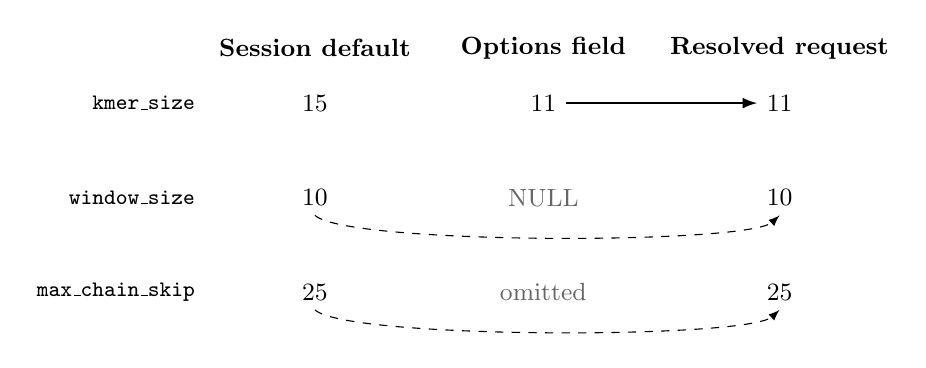
\begin{tikzpicture}[font=\small, >=latex]
  \node[font=\small\bfseries] at (3.9,.7) {Session default};
  \node[font=\small\bfseries] at (6.8,.7) {Options field};
  \node[font=\small\bfseries] at (9.8,.7) {Resolved request};
  \node[anchor=east,font=\footnotesize\ttfamily] at (2.5,0) {kmer\_size};
  \node[anchor=east,font=\footnotesize\ttfamily] at (2.5,-1.2) {window\_size};
  \node[anchor=east,font=\footnotesize\ttfamily] at (2.5,-2.4) {max\_chain\_skip};
  \node (d1) at (3.9,0) {15};
  \node (d2) at (3.9,-1.2) {10};
  \node (d3) at (3.9,-2.4) {25};
  \node (o1) at (6.8,0) {11};
  \node[text=black!60] at (6.8,-1.2) {NULL};
  \node[text=black!60] at (6.8,-2.4) {omitted};
  \node (r1) at (9.8,0) {11};
  \node (r2) at (9.8,-1.2) {10};
  \node (r3) at (9.8,-2.4) {25};
  \draw[->,thick] (o1.east) -- (r1.west);
  \draw[->,dashed] (d2.south)
    .. controls (4.3,-1.8) and (9.4,-1.8) .. (r2.south);
  \draw[->,dashed] (d3.south)
    .. controls (4.3,-3.0) and (9.4,-3.0) .. (r3.south);
\end{tikzpicture}
\caption{A non-NULL field overrides its default. Dashed arrows show
inheritance for NULL and omitted fields. Route checks and parameter
adjustments follow this merge.}
\label{fig:appendix-options-precedence}
\end{figure}

Omitting the third argument, supplying \texttt{public.aligner\_options()},
and supplying \texttt{NULL::public.bioseq\_aligner\_options} all request
the inherited option set. A NULL sequence operand has a different meaning:
it produces no alignment.

Options must become a constant of the exact composite type during planning.
The immutable constructor with constant arguments satisfies this rule.
A typed composite string literal or a constant expression that folds to the
same type is also accepted. A raw composite literal must contain all 36
positions, including empty positions for NULLs. The named constructor is
easier to maintain. Column values, subqueries, volatile wrappers, and
parameters that remain unresolved in a generic prepared plan are unsupported
options expressions.

An ordinary \texttt{BioseqScan} captures the GUC values and overrides in its
plan. A \texttt{BioseqBatchJoin}, including searches with slices or
concatenated sequence arguments,
resolves GUC values again during executor initialization and reapplies the
constant overrides. Changing the relevant alignment GUCs invalidates cached
plans. These routes therefore share the precedence rule while resolving
defaults at different points.

The displayed defaults are requested values. For a short pair, the ordinary
pair adjustment can reduce $k$, $w$, the chain-score threshold, and the seed
threshold when their values equal $15,10,40,3$. Explicitly writing those same
four values does not disable the adjustment. An indexed route must prepare
query sketches compatible with its stored lookup.

\subsection{Complete field reference}
\label{sec:appendix-options-fields}

Every constructor field is nullable. \textbf{I} means SQL \texttt{integer},
\textbf{D} means \texttt{double precision}, and \textbf{B} means
\texttt{boolean}. The four D fields are converted to single precision in
the alignment parameters. In the table, prepend
\texttt{bioseq.aligner.} to each GUC suffix.

\textbf{The numeric intervals below are the corresponding GUC bounds.}
The options constructor and override decoder do not enforce these intervals
for ordinary numeric fields. Algorithm codes and the index-policy code are
checked explicitly. Later kernels impose additional conditions, so even a
value within its GUC interval need not work with every algorithm. Use the
listed intervals together with the route restrictions below.

\begingroup
\footnotesize
\setlength{\tabcolsep}{3pt}
\renewcommand{\arraystretch}{1.12}
\begin{longtable}{@{}>{\raggedright\arraybackslash}p{.27\linewidth}
  >{\raggedright\arraybackslash}p{.69\linewidth}@{}}
\caption{All options fields in composite order. Defaults are initial session
values, except for the independent index policy.}
\label{tab:appendix-options-fields}\\
\toprule
\textbf{Field and type} & \textbf{GUC suffix, default, range, and effect}\\
\midrule
\endfirsthead
\multicolumn{2}{l}{\textit{Search options, continued}}\\
\toprule
\textbf{Field and type} & \textbf{GUC suffix, default, range, and effect}\\
\midrule
\endhead
\midrule
\multicolumn{2}{r}{\textit{Continued on the next page}}\\
\endfoot
\bottomrule
\endlastfoot
\path{kmer_size} (I) &
  \path{minimizer.kmer_size}. Default 15, GUC range $1\ldots64$.
  Length of each $k$-mer in sequence symbols.\\
\path{window_size} (I) &
  \path{minimizer.window_size}. Default 10, GUC range $1\ldots1024$.
  Number of consecutive $k$-mers in a minimizer window.\\
\path{max_gap} (I) &
  \path{chaining.maximum_gap}. Default 5000, GUC range $1\ldots2^{30}$.
  Distance limit used by chaining. The scalar chainer raises it to at least
  the bandwidth.\\
\path{max_gap_ref} (I) &
  \path{chaining.maximum_reference_gap}. Default $-1$, GUC range
  $-1\ldots2^{30}$. Stored reference-gap option, currently unused by
  execution.\\
\path{bandwidth} (I) &
  \path{chaining.bandwidth}. Default 500, GUC range $1\ldots2^{20}$.
  Diagonal-band setting for the algorithms that use it.\\
\path{bandwidth_long} (I) &
  \path{chaining.long_join_bandwidth}. Default 0, GUC range
  $0\ldots2^{20}$. Stored long-join option, currently unused by execution.\\
\path{max_chain_skip} (I) &
  \path{chaining.maximum_skipped_anchors}. Default 25, GUC range
  $0\ldots2^{20}$. Early-stop limit interpreted by the selected chainer.
  SQL SIMD chaining requires a positive value.\\
\path{max_chain_iter} (I) &
  \path{chaining.maximum_predecessors}. Default 5000, GUC range
  $1\ldots2^{22}$. Predecessor-scan limit for scan-based chainers.
  The scalar chainer can inspect one additional candidate. RMQ does not
  use this field.\\
\path{min_seed_count} (I) &
  \path{chaining.minimum_seed_count}. Default 3, GUC range
  $0\ldots2^{20}$. Minimum accepted chain seed count.\\
\path{min_chain_score} (I) &
  \path{chaining.minimum_score}. Default 40, GUC range $0\ldots2^{20}$.
  Minimum accepted chain score.\\
\path{chain_gap_scale} (D) &
  \path{chaining.gap_penalty_scale}. Default 0.8, GUC range $0\ldots100$.
  Scale for the chaining gap penalty.\\
\path{chain_skip_scale} (D) &
  \path{chaining.skip_penalty_scale}. Default 0, GUC range $0\ldots100$.
  Scale for the chaining skip (distance) penalty.\\
\path{mask_level} (D) &
  \path{secondary.overlap_threshold}. Default 0.5, GUC range $0\ldots1$.
  Overlap threshold used when assigning secondary mappings.\\
\path{mask_len} (I) &
  \path{secondary.uncovered_length_limit}. Default $2^{31}-1$,
  GUC range $0\ldots2^{31}-1$. Uncovered-length limit in that assignment.\\
\path{pri_ratio} (D) &
  \path{secondary.score_ratio_threshold}. Default 0.8, GUC range
  $0\ldots1$. Secondary-to-primary score threshold. Zero bypasses this
  secondary filtering step, including its count limit.\\
\path{best_n} (I) &
  \path{secondary.maximum_count}. Default 5, GUC range $0\ldots1024$.
  Maximum secondary alignments kept by the filter, counted together across
  all primary alignments in its input. It is not an SQL result-row limit.\\
\path{match_score} (I) &
  \path{scoring.match_score}. Default 2, GUC range $1\ldots127$.
  Score for a matching base.\\
\path{mismatch_pen} (I) &
  \path{scoring.mismatch_penalty}. Default 4, GUC range $1\ldots127$.
  Penalty for a mismatching base.\\
\path{gap_open1} (I) &
  \path{scoring.short_gap_open_penalty}. Default 4, GUC range
  $0\ldots127$. First gap-opening penalty.\\
\path{gap_ext1} (I) &
  \path{scoring.short_gap_extension_penalty}. Default 2, GUC range
  $0\ldots127$. First gap-extension penalty.\\
\path{gap_open2} (I) &
  \path{scoring.long_gap_open_penalty}. Default 24, GUC range
  $0\ldots127$. Second gap-opening penalty, used by KSW2.\\
\path{gap_ext2} (I) &
  \path{scoring.long_gap_extension_penalty}. Default 1, GUC range
  $0\ldots127$. Second gap-extension penalty, used by KSW2.\\
\path{sc_ambi} (I) &
  \path{scoring.ambiguous_base_penalty}. Default 1, GUC range
  $0\ldots127$. Penalty for ambiguous bases.\\
\path{zdrop} (I) &
  \path{scoring.z_drop_threshold}. Default 400, GUC range
  $-1\ldots2^{20}$. KSW2 Z-drop threshold, or BlockAligner X-drop
  threshold for end extensions.\\
\path{end_bonus} (I) &
  \path{scoring.end_bonus}. Default $-1$, GUC range $-1\ldots2^{20}$.
  KSW2 sequence-end bonus. $-1$ disables the bonus.\\
\path{max_occ} (I) &
  \path{seeding.maximum_occurrence}. Default 500, GUC range
  $1\ldots2^{24}$. Excludes seed keys whose target occurrence count
  exceeds this limit.\\
\path{mid_occ} (I) &
  \path{seeding.intermediate_occurrence_threshold}. Default 500,
  GUC range $1\ldots2^{24}$. Stored intermediate threshold, currently
  unused by execution.\\
\path{block_min_size} (I) &
  \path{block_alignment.minimum_block_size}. Default 32, GUC range
  $8\ldots4096$. Minimum adaptive block size for BlockAligner.\\
\path{block_max_size} (I) &
  \path{block_alignment.maximum_block_size}. Default 256, GUC range
  $8\ldots16384$. Maximum adaptive block size for BlockAligner.\\
\path{chaining_algorithm} (I) &
  \path{chaining.algorithm}. Default 0, accepted codes $0\ldots3$.
  See Table~\ref{tab:appendix-options-algorithms}.\\
\path{base_alignment_algorithm} (I) &
  \path{base_alignment.algorithm}. Default 1, accepted codes $0,1$.
  See Table~\ref{tab:appendix-options-algorithms}.\\
\path{minimizer_algorithm} (I) &
  \path{minimizer.algorithm}. Default 0, accepted codes $0\ldots4$.
  See Table~\ref{tab:appendix-options-algorithms}.\\
\path{vulkan_enabled} (B) &
  \path{vulkan.enabled}. Default \texttt{true}, values
  \texttt{true}/\texttt{false}. Allows Vulkan execution. An explicit true
  value also has the prefilter meaning described below.\\
\path{vulkan_seed_hits_enabled} (B) &
  \path{vulkan.seed_lookup.enabled}. Default \texttt{false}, values
  \texttt{true}/\texttt{false}. Selects Vulkan seed lookup.\\
\path{vulkan_index_cache_enabled} (B) &
  \path{vulkan.index_cache.enabled}. Default \texttt{true}, values
  \texttt{true}/\texttt{false}. Controls caching of GPU index uploads.\\
\path{index_read_requirement} (I) &
  No GUC. Default 0, accepted codes $0\ldots2$.
  Selects the persisted-index policy described below.\\
\end{longtable}
\endgroup

The three stored but unused numeric options remain part of the public
composite. Assigning them currently does not implement a separate reference
gap, a long-join pass, or intermediate occurrence filtering.

\subsection{Algorithm codes and route restrictions}
\label{sec:appendix-options-algorithms}

Algorithm fields use integer codes. Their GUC counterparts use the names in
Table~\ref{tab:appendix-options-algorithms}. A valid code selects a family,
but does not guarantee that the input, hardware, or other choices are
compatible. Sections~\ref{sec:configured-cpu-minimizers} and
\ref{sec:chaining-bioseqdb} explain the algorithm families.

\begin{table}[htbp]
\centering
\footnotesize
\begin{tabularx}{\linewidth}{@{}p{.30\linewidth}rX@{}}
\toprule
\textbf{Options field} & \textbf{Code} & \textbf{GUC value}\\
\midrule
\path{minimizer_algorithm} & 0 & \path{scalar}\\
 & 1 & \path{simd_minimap2_reference}\\
 & 2 & \path{two_stack_nthash}\\
 & 3 & \path{vulkan_minimap_integer}\\
 & 4 & \path{bounded_nthash_simd}\\
\midrule
\path{chaining_algorithm} & 0 & \path{scalar_minimap2}\\
 & 1 & \path{simd_minimap2}\\
 & 2 & \path{range_minimum_query}\\
 & 3 & \path{vulkan_tiled_dynamic_programming}\\
\midrule
\path{base_alignment_algorithm} & 0 & \path{ksw2}\\
 & 1 & \path{block_aligner}\\
\bottomrule
\end{tabularx}
\caption{Integer options codes and their named GUC equivalents.}
\label{tab:appendix-options-algorithms}
\end{table}

Keep the following restrictions in mind:
\begin{itemize}
  \item Bounded ntHash SIMD requires DNA4, $k=15$, and $w=10$.
    SQL SIMD chaining uses the bounded policy and requires positive
    \texttt{max\_chain\_skip} and \texttt{max\_chain\_iter}.
    Unsupported SIMD chaining is not retried as scalar chaining.
  \item BlockAligner uses the first gap-penalty pair. Both penalties must
    be positive and their sum must not exceed 128. After widening to at least
    the active lane count, its minimum and maximum block sizes must be
    powers of two with minimum no larger than maximum. End extension
    requires a nonnegative \texttt{zdrop}. Invalid BlockAligner contracts
    can terminate the backend, so arbitrary numeric options should not be
    used to probe its limits.
  \item Biological Vulkan stages require the complete supported execution
    route. The options object exposes only three Vulkan Boolean fields.
    Fused frontend, GPU index build, and GPU alignment extension are
    controlled by separate GUCs. Selecting a Vulkan algorithm code alone
    is insufficient.
  \item In an ordinary scan with an eligible exact edit-distance filter,
    explicit \texttt{vulkan\_enabled => true} requests the standalone
    Vulkan prefilter. Merely inheriting the default enabled GUC does not
    make this request. Consequently, that explicit option and a session
    \texttt{SET} are not always equivalent.
\end{itemize}

The options object does not contain output-stage flags. Requesting CIGAR,
edit distance, divergence, or mapping quality through the SQL result helpers
determines the extra work. Choosing a base aligner alone does not force base
alignment for a coordinate-only search. The internal batched KSW2 route is
not an additional SQL algorithm code.

\subsection{Per-call persisted-index policy}
\label{sec:appendix-options-index-policy}

\begin{description}
  \item[0: \texttt{allow}.] Follow the normal index-reading policy. A
    compatible persisted lookup may be used, and an unavailable or
    inapplicable lookup may be recomputed. This value does not override
    \texttt{bioseq.index.sequence\_read.enabled} to enable index reads.
  \item[1: \texttt{require\_absent}.] Disable persisted target-index reads
    for this search. It does not delete an existing index. Separate
    persistence settings can still allow a recomputed index to be written.
  \item[2: \texttt{require\_compatible\_persisted}.] Require a compatible
    persisted generation. A recomputed target index or a transient assembled
    index in memory does not satisfy the requirement. Reusing a retained
    reader for the compatible persisted generation does satisfy it.
    The current prepared-reader route
    belongs to \texttt{BioseqBatchJoin}. An ordinary executable
    \texttt{BioseqScan} rejects this requirement.
\end{description}

A transformed target, such as a slice or concatenation, must be searched
through its evaluated logical view.
Its route forces \texttt{require\_absent} and rejects code 2. For an
untransformed stored target, compatibility includes its source generation,
alphabet, minimizer scheme, producer, and sketch parameters.

\subsection{Search examples}
\label{sec:appendix-options-examples}

Assume \texttt{refs} and \texttt{queries} are BioSeqDB sequence tables with
an \texttt{id} column and a \texttt{seq} column of type
\texttt{bioseq.seq('dna4',32)}. Listing~\ref{lst:appendix-options-join}
sets a session $k$-mer default of 15, then overrides it to 11 for the join.
The other explicitly selected values apply only to this predicate.

\par\noindent\begin{minipage}{\linewidth}
\begin{lstlisting}[style=bioseq-appendix-sql,
  caption={Override session defaults for a sequence join.},
  label={lst:appendix-options-join}]
BEGIN;
SET LOCAL bioseq.aligner.minimizer.kmer_size = 15;
SELECT r.id, q.id
FROM refs AS r JOIN queries AS q
  ON public.mmsearch(r.seq, q.seq,
       public.aligner_options(
         kmer_size => 11, window_size => 5,
         minimizer_algorithm => 0,
         chaining_algorithm => 0,
         index_read_requirement => 1));
COMMIT;
\end{lstlisting}
\end{minipage}

A constant query uses the same third argument. The short-query example
below explicitly sets sketch and chain thresholds. It requests an alignment
search, not an exact substring test.

\par\noindent\begin{minipage}{\linewidth}
\begin{lstlisting}[style=bioseq-appendix-sql,
  caption={Search stored sequences with a typed constant query.},
  label={lst:appendix-options-constant-query}]
SELECT r.id
FROM refs AS r
WHERE public.mmsearch(
  r.seq,
  'ACGTTGCAAGTCGATCGTACGATGCTAGCTAGGCTAACGT'
    ::bioseq.seq('dna4',32),
  public.aligner_options(
    kmer_size => 7, window_size => 1,
    min_seed_count => 1, min_chain_score => 7,
    minimizer_algorithm => 0, chaining_algorithm => 0,
    index_read_requirement => 1));
\end{lstlisting}
\end{minipage}

To retain every session alignment default while giving the third argument
explicitly, use the typed NULL form:

\par\noindent\begin{minipage}{\linewidth}
\begin{lstlisting}[style=bioseq-appendix-sql,
  caption={Use the three-argument overload without overrides.},
  label={lst:appendix-options-null}]
SELECT r.id, q.id
FROM refs AS r JOIN queries AS q
  ON public.mmsearch(
    r.seq, q.seq, NULL::public.bioseq_aligner_options);
\end{lstlisting}
\end{minipage}

\section{Read, search, and write sequences}
\label{sec:appendix-quick-start}

This example stores DNA beside ordinary metadata, reads a small part of each
sequence, and searches the stored targets. The examples assume that the
extension's installation schema is \texttt{public}. Sequence types and helper
functions use the fixed \texttt{bioseq} schema.

\subsection{Install the extension and create a table}

Install the extension in the database where the application will run. The
catalog query confirms its version in that database.

\par\noindent\begin{minipage}{\linewidth}
\begin{lstlisting}[style=bioseq-appendix-sql]
CREATE EXTENSION bioseq;
SELECT extname, extversion
FROM pg_extension
WHERE extname = 'bioseq';

CREATE TABLE sample_reads (
    read_id bigint GENERATED ALWAYS AS IDENTITY PRIMARY KEY,
    sample_id text NOT NULL,
    collected_on date NOT NULL,
    passed_qc boolean NOT NULL DEFAULT false,
    sequence bioseq.seq('dna4', 64) NOT NULL
) USING bioseq;
\end{lstlisting}
\end{minipage}

\begin{itemize}
  \item \texttt{dna4} binds the sequence to the symbols A, C, G, and T.
    Ordinary SQL input containing N fails for this alphabet.
  \item \texttt{64} is the width of a packed storage unit, in bits. It is
    neither a length limit nor the number of bases in the sequence.
  \item \texttt{USING bioseq} selects the sequence-aware table access method.
    A heap table can hold sequence values, but it does not provide the same
    table storage and custom search route.
\end{itemize}

A build may normalize accepted storage widths to 64 bits. Inspect the actual
column declaration when comparing widths; the alphabet remains unchanged.
The \texttt{psql} command \texttt{\textbackslash d+ sample\_reads} also shows
the table's access method.

\par\noindent\begin{minipage}{\linewidth}
\begin{lstlisting}[style=bioseq-appendix-sql]
SELECT a.attname AS column_name,
       format_type(a.atttypid, a.atttypmod) AS active_type
FROM pg_attribute AS a
WHERE a.attrelid = 'sample_reads'::regclass
  AND a.attnum > 0 AND NOT a.attisdropped
ORDER BY a.attnum;
\end{lstlisting}
\end{minipage}

\subsection{Choose a write policy}

For ordinary application writes, enable insert maintenance in the writing
transaction. This switch permits maintenance of indexes whose table policy
requests updates on insertion. It does not change a manually maintained
index's policy. Section~\ref{sec:appendix-indexes} lists those policies and
their interaction with the switch.

\par\noindent\begin{minipage}{\linewidth}
\begin{lstlisting}[style=bioseq-appendix-sql]
BEGIN;
SET LOCAL bioseq.index.insert_maintenance.enabled = on;
INSERT INTO sample_reads
    (sample_id, collected_on, passed_qc, sequence)
VALUES
    ('sample-a', DATE '2026-08-01', true,
     'TCACTGTAGGATCGTAGCTAGTCCGTACTGTAGCTGATCGTAGC'
     'CCTAGTCACTGTAGCCTGATCGTAGCTAGTCACTGTAGCCATACCTGAA'),
    ('sample-a', DATE '2026-08-01', true,
     'CCCCAACTTAGTCACTTCTCAAAAATTACTCTCTCATCATCATC'
     'TACTCCTAGTCACTGTAGCCTGATCGTAGCTAGTCACACACACCCCAAA'),
    ('sample-b', DATE '2026-08-02', false,
     'GGGGGTCACTTCTCAAAAATTAGGGGGGGGGTAGTCACTGTAG'
     'CCTGATCGTAGCTAGGACACATATCATCATCTACTCCTATCATCATCTACTCCTA')
RETURNING read_id, sample_id, bioseq.len(sequence) AS bases;
COMMIT;
\end{lstlisting}
\end{minipage}

Adjacent SQL string literals separated by a newline form one value in this
listing. \texttt{SET LOCAL} lasts until the transaction ends. Use ordinary
\texttt{SET} when the same policy should apply to later transactions in the
connection.

For a bulk import, turn maintenance off while loading, then build the required
index once. The following call rebuilds the minimizers-per-fragment index for
the relation.

\par\noindent\begin{minipage}{\linewidth}
\begin{lstlisting}[style=bioseq-appendix-sql]
SET bioseq.index.insert_maintenance.enabled = off;
-- Load rows with COPY, application batches, or bioseq.load.
SELECT bioseq.update_index(
    'sample_reads'::regclass, 'minimizers_per_fragment'
);
RESET bioseq.index.insert_maintenance.enabled;
\end{lstlisting}
\end{minipage}

The other minimizer recipe is \texttt{minimizers\_per\_sequence}. Import
procedures should record the table, recipe, and result of the rebuild call.
If the application requires a ready stored index, publish the dataset only
after the rebuild succeeds. A staging table allows the load and rebuild to
finish before a short application-level publication transaction. The
experimental grouped-SoA mode rejects ordinary per-tuple minimizer
maintenance. There is a streamed-load exception: \texttt{bioseq.load} can
rebuild eligible update-on-insert indexes after flushing the complete load,
subject to the grouped-format requirements in
Section~\ref{sec:appendix-indexes}.

\subsection{Read lengths, counts, and previews}

Read sequence metadata or a slice when that is all the client needs. The
following query returns lengths and symbol counts without returning the
complete sequence as text.

\par\noindent\begin{minipage}{\linewidth}
\begin{lstlisting}[style=bioseq-appendix-sql]
SELECT read_id, sample_id,
       bioseq.len(sequence) AS symbols,
       bioseq.unit_len(sequence) AS packed_units,
       bioseq.symbol_count(sequence, 'A') AS a_bases
FROM sample_reads
WHERE passed_qc
ORDER BY read_id;

SELECT read_id,
       sequence[:12]::text AS first_twelve,
       sequence[-12:]::text AS last_twelve
FROM sample_reads
ORDER BY read_id;
\end{lstlisting}
\end{minipage}

\begin{itemize}
  \item \texttt{len} returns the number of symbols; \texttt{unit\_len}
    returns the number of packed units. Both return \texttt{bigint}.
  \item \texttt{symbol\_count} counts the requested symbol. Its ability to
    use stored counts depends on the available index and selected plan.
  \item Slice bounds are zero-based and half-open: \texttt{[:12]} selects
    positions 0 through 11. \texttt{[-12:]} selects up to twelve final
    symbols. Short values are clamped to their available range.
\end{itemize}

Convert the complete value only when it is needed, for example
\texttt{SELECT sequence::text FROM sample\_reads WHERE read\_id = 1}.
Sections~\ref{sec:appendix-sequence-type}
and~\ref{sec:appendix-sequence-transforms} give the full rules for widths,
negative bounds, and transformations.

\subsection{Search targets and return alignment rows}

Put the stored target first in \texttt{mmsearch}, followed by a query with a
compatible bound alphabet. Ordinary metadata filters can remain beside the
search predicate.

\par\noindent\begin{minipage}{\linewidth}
\begin{lstlisting}[style=bioseq-appendix-sql]
SELECT read_id, sample_id,
       bioseq.query_start(read_id) AS query_start,
       bioseq.query_end(read_id) AS query_end,
       bioseq.target_start(read_id) AS target_start,
       bioseq.target_end(read_id) AS target_end,
       bioseq.cigar(read_id) AS cigar
FROM sample_reads
WHERE sample_id = 'sample-a'
  AND collected_on >= DATE '2026-08-01'
  AND passed_qc
  AND public.mmsearch(
      sequence,
      'CTAGTCACTGTAGCCTGATCGTAGCTAGT'::bioseq.seq('dna4', 64),
      public.aligner_options(best_n => 3)
  )
ORDER BY read_id, target_start, target_end;
\end{lstlisting}
\end{minipage}

The coordinate functions read the current alignment. Their \texttt{read\_id}
argument identifies the table alias owning this one search; its numeric value
is not used to find an alignment in a second table. A stored row can therefore
appear several times with different coordinates. Coordinates are zero-based
and half-open, so an interval's length is \texttt{end - start}.

The optional object changes the call's settings. Here \texttt{best\_n}
limits retained secondary regions when secondary filtering is active. It
does not limit matching table rows or all primary regions. The two-argument
form uses session defaults. Section~\ref{sec:appendix-search-options}
explains every object field, its corresponding default, and the restrictions
on constant options.

\subsection{Check the chosen plan}

Start with plain \texttt{EXPLAIN}, which does not execute the statement.
Explain the same filters and projections used by the application.

\par\noindent\begin{minipage}{\linewidth}
\begin{lstlisting}[style=bioseq-appendix-sql]
EXPLAIN (VERBOSE, COSTS OFF)
SELECT read_id,
       bioseq.len(sequence),
       bioseq.symbol_count(sequence, 'A')
FROM sample_reads
WHERE passed_qc;

EXPLAIN (VERBOSE, COSTS OFF)
SELECT read_id
FROM sample_reads
WHERE passed_qc
  AND public.mmsearch(
      sequence,
      'CTAGTCACTGTAGCCTGATCGTAGCTAGT'::bioseq.seq('dna4', 64)
  );
\end{lstlisting}
\end{minipage}

For the search, check for \texttt{Custom Scan (BioseqScan)}. The plan's
projected columns, metadata reads, index-read requirement, operand evaluation,
and pipeline describe what this statement requests. Highway dispatch fields
describe CPU implementations available to that plan. Adding
\texttt{ANALYZE} to \texttt{EXPLAIN} runs the statement and adds execution
information; it also runs writes or remote requests when those are part of the
statement.

If the search has no owning custom scan, check the table's access method,
operand types, visible top-level predicate, and enabled custom-scan path.
Then check the index state against the selected read policy. Missing index
coverage can permit recomputation under an allowing policy; it does not by
itself mean that a custom scan is impossible. The ordinary SQL function is
not an alternative row-by-row search implementation.
Section~\ref{sec:appendix-explain} explains the plan fields in detail.

\subsection{Update, delete, and bind application parameters}

Update metadata and sequence values in the same SQL statement. For indexes
maintained on insertion, the write switch also applies to the replacement
row created by an update.

\par\noindent\begin{minipage}{\linewidth}
\begin{lstlisting}[style=bioseq-appendix-sql]
BEGIN;
SET LOCAL bioseq.index.insert_maintenance.enabled = on;
UPDATE sample_reads
SET passed_qc = true,
    sequence = 'ACGTACGTACGTACGTACGTACGTACGTACGT'
WHERE read_id = 3;
COMMIT;

DELETE FROM sample_reads WHERE read_id = 3;
\end{lstlisting}
\end{minipage}

After maintenance-off inserts or sequence updates, rebuild the required
stored index before relying on its coverage. Deletion changes row visibility;
it does not require applications to identify internal index chunks themselves.

Applications should bind query text as data. The following prepared statement
keeps the sample name and query sequence separate from SQL text. The query
parameter is bound to the target alphabet before search execution.

\par\noindent\begin{minipage}{\linewidth}
\begin{lstlisting}[style=bioseq-appendix-sql]
PREPARE find_sample_reads(text, text) AS
SELECT read_id, sample_id,
       bioseq.target_start(read_id) AS target_start,
       bioseq.target_end(read_id) AS target_end
FROM sample_reads
WHERE sample_id = $1
  AND public.mmsearch(sequence, $2::bioseq.seq('dna4', 64))
ORDER BY read_id, target_start, target_end;

EXECUTE find_sample_reads(
    'sample-a', 'CTAGTCACTGTAGCCTGATCGTAGCTAGT'
);
DEALLOCATE find_sample_reads;
\end{lstlisting}
\end{minipage}

Drop \texttt{sample\_reads} when the exercise is finished.
Keep the write policy, index recipe, and
effective search options explicit in an application, and confirm the actual
plan before measuring representative searches.

\section{The sequence column type}
\label{sec:appendix-sequence-type}

The type \texttt{bioseq.seq} stores a sequence together with the information
needed to interpret its symbols. A column declaration such as
\texttt{bioseq.seq('dna4',64)} specifies an alphabet and a packed storage-unit
width. The number 64 is neither a sequence-length limit nor the number of bits
used for each base. The examples assume that the extension has been installed
in the current database.

\subsection{Choose an alphabet and a packed width}

Choose the alphabet from the data that the column must preserve:
\begin{itemize}
  \item \texttt{dna4} represents A, C, G, and T. Use it when every input
    sequence consists of these four bases.
  \item \texttt{dna5} also represents N. Use it when an unknown base must keep
    its place in the sequence. This alphabet needs a build that registers it.
  \item A typed SQL input cast checks the symbols. Removing an unsupported
    symbol beforehand changes the sequence and moves every later position.
    It is a data transformation, not a harmless way to suppress an error.
\end{itemize}

This table is used throughout the first tutorial. Its primary key identifies
the record; its sequence column has an explicit alphabet.

\par\noindent\begin{minipage}{\linewidth}
\begin{lstlisting}[style=bioseq-appendix-sql]
CREATE TABLE resolved_reads (
    read_id bigint PRIMARY KEY,
    sequence bioseq.seq('dna4', 64) NOT NULL
) USING bioseq;

SET bioseq.index.insert_maintenance.enabled = on;
INSERT INTO resolved_reads VALUES
    (1, 'ACGTACGT'::bioseq.seq('dna4', 64)),
    (2, 'TTAA'::bioseq.seq('dna4', 64));
RESET bioseq.index.insert_maintenance.enabled;

SELECT read_id, sequence::text, bioseq.len(sequence)
FROM resolved_reads
ORDER BY read_id;
\end{lstlisting}
\end{minipage}

The output contains the same symbols that were inserted, with lengths 8 and
4. The maintenance setting permits enabled per-insert index work; it does not
select an alphabet or change the sequence type. Section~\ref{sec:appendix-configuration}
describes the index controls and their restrictions.

The accepted width arguments are 8, 16, 32, and 64 bits. A normal build
normalizes all four to 64-bit packed units. A build with all coordinate-width
variants enabled can retain the other widths. Therefore:
\begin{itemize}
  \item Treat the width as a request for a storage representation. Inspect the
    installed type modifier before comparing widths.
  \item Do not confuse packed units with bytes, bases, or SIMD lanes.
    Changing this argument does not by itself select a SIMD algorithm.
  \item Keep the default width unless measurements of the intended workload
    give a reason to change it.
\end{itemize}

\subsection{Inspect the stored modifier and name the measurement units}

The following probe distinguishes the requested widths from the modifiers
that PostgreSQL actually records. It deliberately puts the same 100-base
value in every column.

\par\noindent\begin{minipage}{\linewidth}
\begin{lstlisting}[style=bioseq-appendix-sql]
CREATE TABLE width_probe (
    id integer PRIMARY KEY,
    w8  bioseq.seq('dna4', 8),
    w16 bioseq.seq('dna4', 16),
    w32 bioseq.seq('dna4', 32),
    w64 bioseq.seq('dna4', 64)
) USING bioseq;

SELECT attname, format_type(atttypid, atttypmod) AS stored_type
FROM pg_attribute
WHERE attrelid = 'width_probe'::regclass
  AND attnum > 0 AND NOT attisdropped
ORDER BY attnum;
\end{lstlisting}
\end{minipage}

\par\noindent\begin{minipage}{\linewidth}
\begin{lstlisting}[style=bioseq-appendix-sql]
INSERT INTO width_probe VALUES (
    1,
    repeat('ACGT', 25)::bioseq.seq('dna4', 8),
    repeat('ACGT', 25)::bioseq.seq('dna4', 16),
    repeat('ACGT', 25)::bioseq.seq('dna4', 32),
    repeat('ACGT', 25)::bioseq.seq('dna4', 64)
);

SELECT bioseq.len(w8) AS symbols,
       bioseq.unit_len(w8) AS units_8,
       bioseq.unit_len(w16) AS units_16,
       bioseq.unit_len(w32) AS units_32,
       bioseq.unit_len(w64) AS units_64,
       w8::text = w64::text AS same_symbols
FROM width_probe;

DROP TABLE width_probe;
\end{lstlisting}
\end{minipage}

\texttt{bioseq.len} returns the number of symbols as a \texttt{bigint}.
\texttt{bioseq.unit\_len} returns the number of packed units needed for the
value's alphabet and width, also as a \texttt{bigint}. For DNA4, a 64-bit unit
holds 32 bases, so 100 bases need four units. In the normal build all four
unit counts above are four, and \texttt{same\_symbols} is true. These counts
do not include value headers, relation pages, or compression overhead; they
are not measurements of physical disk usage.

An empty sequence has zero symbols and zero packed units. It is different
from SQL \texttt{NULL}, which means that the value is missing.

\par\noindent\begin{minipage}{\linewidth}
\begin{lstlisting}[style=bioseq-appendix-sql]
SELECT bioseq.len(''::bioseq.seq('dna4', 64)) AS symbols,
       bioseq.unit_len(''::bioseq.seq('dna4', 64)) AS units,
       ''::bioseq.seq('dna4', 64) IS NULL AS is_missing;
-- symbols = 0; units = 0; is_missing = false
\end{lstlisting}
\end{minipage}

\subsection{Bind client inputs and convert widths}

Pass client sequence data as a text parameter and cast it explicitly at the
database boundary. This makes the intended alphabet visible and avoids
relying on how a client driver describes a parameter.

\par\noindent\begin{minipage}{\linewidth}
\begin{lstlisting}[style=bioseq-appendix-sql]
PREPARE insert_resolved_read(bigint, text) AS
INSERT INTO resolved_reads (read_id, sequence)
VALUES ($1, $2::bioseq.seq('dna4', 64));

EXECUTE insert_resolved_read(3, 'ACGTACGT');
DEALLOCATE insert_resolved_read;

SELECT ('ACGT'::bioseq.seq('dna4', 16)
               ::bioseq.seq('dna4', 64))::text;
-- ACGT
\end{lstlisting}
\end{minipage}

A cast between widths of the same alphabet preserves the symbols. It can be
a no-op when the build normalizes both widths. Where the widths differ, the
cast changes the requested representation; a lazy sequence need not be
copied into a new packed array immediately.

An alphabet is \emph{bound} when it is recorded in the sequence value.
Casting directly between two different bound alphabets is rejected, even
when the particular symbols would fit both alphabets. For example, a bound
DNA4 value cannot be cast directly to bound DNA5. Convert through text when
an alphabet change is intentional, and validate the destination contract.
The following optional example requires DNA5 support:

\par\noindent\begin{minipage}{\linewidth}
\begin{lstlisting}[style=bioseq-appendix-sql]
WITH candidates(sequence) AS (
    VALUES ('ACGT'::bioseq.seq('dna5', 64)),
           ('ACNT'::bioseq.seq('dna5', 64))
)
SELECT CASE WHEN sequence::text ~ '^[ACGT]*$'
            THEN sequence::text::bioseq.seq('dna4', 64)
       END AS resolved_sequence
FROM candidates;
\end{lstlisting}
\end{minipage}

The first result is ACGT; the second is \texttt{NULL}. The expression makes
the rejection policy explicit. If N is meaningful in the application, retain
DNA5 instead of changing its alphabet.

\subsection{Unbound values and client output}

A SQL expression can have the bare type \texttt{bioseq.seq}, without a type
modifier. This alone does not prove whether the value has a bound alphabet:
the value also carries this information. Current external-provider results
start as unbound ASCII sequences. Provider relation options do not turn
these results into a selected packed alphabet and width.

Length and text output are useful before binding. Alphabet-dependent
operations, such as returning a typed letter, creating a letter array, or
computing a reverse complement, need a bound alphabet. Bind and validate an
external value before using those operations. This example requests the
first 100 bases of the human mitochondrial reference from UCSC:

\par\noindent\begin{minipage}{\linewidth}
\begin{lstlisting}[style=bioseq-appendix-sql]
SELECT bioseq.len(sequence) AS bases, sequence::text
FROM bioseq_external.sequences
WHERE provider = 'ucsc'
  AND assembly_database = 'hg38'
  AND chromosome = 'chrM'
  AND start0 = 0 AND end0 = 100;
\end{lstlisting}
\end{minipage}

The provider example requires the external-provider installation and network
access. With DNA5 available, the expression below gives an explicit
validation boundary before the reverse complement. The text step is also
useful when changing an already bound alphabet; it is not required merely
to bind an unbound value.

\par\noindent\begin{minipage}{\linewidth}
\begin{lstlisting}[style=bioseq-appendix-sql]
SELECT bioseq.reverse_complement(
           sequence::text::bioseq.seq('dna5', 64))::text
FROM bioseq_external.sequences
WHERE provider = 'ucsc'
  AND assembly_database = 'hg38'
  AND chromosome = 'chrM'
  AND start0 = 0 AND end0 = 100;
\end{lstlisting}
\end{minipage}

Keep a sequence typed while the database searches or transforms it. Choose
the output form that the client actually needs:
\begin{itemize}
  \item Use \texttt{sequence::text} to return the complete string.
  \item Use \texttt{bioseq.to\_array(sequence)} only when the client needs a
    \texttt{bioseq.letter[]} array. Each element is a typed symbol.
  \item Use \texttt{sequence[:20]::text} or
    \texttt{sequence[-20:]::text} for a short prefix or suffix. Avoid
    returning a whole chromosome merely to display a preview.
\end{itemize}

\par\noindent\begin{minipage}{\linewidth}
\begin{lstlisting}[style=bioseq-appendix-sql]
SELECT read_id, sequence[:20]::text AS prefix,
       sequence[-20:]::text AS suffix,
       bioseq.to_array(sequence[:4]) AS first_four_letters
FROM resolved_reads
ORDER BY read_id;
\end{lstlisting}
\end{minipage}

\subsection{Compare values and use several sequence columns}

Sequence comparison uses the value's alphabet and logical symbols. Equal
symbols in the same alphabet compare equally across packed widths; physical
packing is not the meaning of equality. Alphabet identity participates in
comparison, so values bound to different alphabets should not be treated as
the same biological value merely because their text looks equal.

The explicit operator form also works when \texttt{bioseq} is absent from
\texttt{search\_path}:

\par\noindent\begin{minipage}{\linewidth}
\begin{lstlisting}[style=bioseq-appendix-sql]
SELECT 'ACGT'::bioseq.seq('dna4', 16)
       OPERATOR(bioseq.=)
       'ACGT'::bioseq.seq('dna4', 64) AS same_sequence;
-- true
\end{lstlisting}
\end{minipage}

A table may contain several sequence columns with different alphabets.
There is no table-wide rule that makes every sequence column DNA4. The
following optional schema requires DNA5 support:

\par\noindent\begin{minipage}{\linewidth}
\begin{lstlisting}[style=bioseq-appendix-sql]
CREATE TABLE paired_sequence_values (
    pair_id bigint PRIMARY KEY,
    resolved bioseq.seq('dna4', 64),
    with_unknowns bioseq.seq('dna5', 64)
) USING bioseq;

INSERT INTO paired_sequence_values VALUES (
    1, 'ACGT'::bioseq.seq('dna4', 64),
    'ACNT'::bioseq.seq('dna5', 64)
);

SELECT pair_id, bioseq.len(resolved), bioseq.len(with_unknowns)
FROM paired_sequence_values;

DROP TABLE paired_sequence_values;
\end{lstlisting}
\end{minipage}

This flexibility does not make mixed-alphabet searches interchangeable.
Choose compatible query and target alphabets explicitly. The separate
question of which search owns a result helper is covered in
Section~\ref{sec:appendix-joins}.

\subsection{Load sequences and inspect metadata work}

The file loader can fill a typed sequence column and map parsed header
fields to scalar columns. The following example assumes an accessible
FASTA file containing only A/C/G/T sequences, with UniProt-style headers
and one sequence destination column:

\par\noindent\begin{minipage}{\linewidth}
\begin{lstlisting}[style=bioseq-appendix-sql]
CREATE TABLE tutorial_loaded_reads (
    accession text NOT NULL,
    seq bioseq.seq('dna4', 64)
) USING bioseq;

SET bioseq.index.insert_maintenance.enabled = on;
SELECT bioseq.load(
    'tutorial_loaded_reads'::regclass,
    'landing_reads.fasta', 'uni_prot',
    ARRAY[('accession', 'accession')::bioseq.column_mapping]
);
RESET bioseq.index.insert_maintenance.enabled;

SELECT accession, bioseq.len(seq) AS bases, seq::text
FROM tutorial_loaded_reads
ORDER BY accession;

DROP TABLE tutorial_loaded_reads;
\end{lstlisting}
\end{minipage}

The path is read by the PostgreSQL server, not the SQL client. The result of
\texttt{bioseq.load} is the loaded-record count. The loader accepts one
bound sequence destination, rejects identity and generated columns, and
requires a default for an unmapped \texttt{NOT NULL} scalar column.

Typed SQL casts and bulk file input do not have identical validation rules.
The bulk reader has path-dependent, permissive handling of unsupported
bytes. Loading N-bearing input into DNA4 can shorten a sequence and shift
coordinates. Validate the input alphabet first when positions must be
preserved. Section~\ref{sec:app-local-ingestion} explains these restrictions,
gzip input, header formats, and the choice between index maintenance during
loading and an index update afterward.

The two statements below ask for different work. The first requests length
and an A count; the second also asks the server to produce the complete
sequence string.

\par\noindent\begin{minipage}{\linewidth}
\begin{lstlisting}[style=bioseq-appendix-sql]
EXPLAIN (ANALYZE, VERBOSE, COSTS OFF)
SELECT bioseq.len(sequence), bioseq.symbol_count(sequence, 'A')
FROM resolved_reads;

EXPLAIN (ANALYZE, VERBOSE, COSTS OFF)
SELECT bioseq.len(sequence), sequence::text
FROM resolved_reads;
\end{lstlisting}
\end{minipage}

On an eligible \texttt{BioseqScan}, \texttt{Bioseq Fetched From Meta}
identifies metadata projections, while \texttt{Bioseq Projected Columns}
lists the supplied columns. A metadata shortcut for one expression does
not remove the payload read required by another expression in the same
query. Inspect the application's complete query.

\subsection{Diagnose input errors and check the schema}

\begin{center}
\small
\begin{tabular}{@{}lp{0.72\linewidth}@{}}
\toprule
SQLSTATE & Meaning in these examples \\
\midrule
\texttt{22P02} & A typed input contains a symbol absent from its alphabet;
  for example, \texttt{'ACGN'::bioseq.seq('dna4',64)}. \\
\texttt{42804} & A cast or assignment tries to change an already bound
  alphabet, or an operation requires an alphabet that is not bound. \\
\texttt{22023} & An unsupported alphabet name or width is used in a type
  modifier. A missing DNA5 build fails here before a DNA4-to-DNA5 cast can
  reach the alphabet-compatibility check. \\
\texttt{42883} & PostgreSQL cannot resolve the requested operator or
  signature; an absent \texttt{bioseq} schema in the search path is one
  possible cause. \\
\bottomrule
\end{tabular}
\end{center}

Check these points before choosing a production schema:
\begin{itemize}
  \item Does the data include N, and does the installed build provide the
    required alphabet?
  \item Which packed width does \texttt{format\_type} actually report?
  \item Do missing values and empty sequences have different meanings in
    the application?
  \item Will insertion maintain the required indexes, or will a later
    explicit update prepare them for search?
  \item Do query and target columns have compatible alphabets?
  \item Which queries need full strings, and which need only lengths,
    counts, or slices?
\end{itemize}

Keep error reports small: record the failing input's identifier, alphabet,
and length instead of printing an entire large sequence. The first tutorial
is now complete; its demonstration table can be removed.

\par\noindent\begin{minipage}{\linewidth}
\begin{lstlisting}[style=bioseq-appendix-sql]
DROP TABLE resolved_reads;
\end{lstlisting}
\end{minipage}

\section{Slices, concatenation, and sequence transforms}
\label{sec:appendix-sequence-transforms}

Sequence operations use zero-based positions and half-open intervals.
They return typed values, so a slice can remain a sequence while it is
reversed, joined to another piece, or searched. Converting the result to
text is a separate request for its symbols.

\subsection{Create a small table and read positions}

\par\noindent\begin{minipage}{\linewidth}
\begin{lstlisting}[style=bioseq-appendix-sql]
CREATE TABLE slice_reads (
    read_id integer PRIMARY KEY,
    sequence bioseq.seq('dna4', 64) NOT NULL
) USING bioseq;

SET bioseq.index.insert_maintenance.enabled = on;
INSERT INTO slice_reads VALUES
    (1, 'ACGTA'::bioseq.seq('dna4', 64)),
    (2, 'TTCCA'::bioseq.seq('dna4', 64)),
    (3, 'GGACT'::bioseq.seq('dna4', 64));
RESET bioseq.index.insert_maintenance.enabled;
\end{lstlisting}
\end{minipage}

\begin{figure}[htbp]
\centering
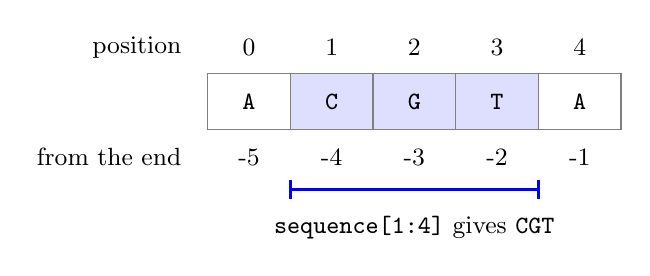
\begin{tikzpicture}[x=1.05cm,y=0.72cm,font=\small]
  \foreach \x/\base/\neg in {0/A/-5,1/C/-4,2/G/-3,3/T/-2,4/A/-1} {
    \ifnum\x>0\ifnum\x<4
      \fill[blue!13] (\x,0) rectangle +(1,1);
    \fi\fi
    \draw[gray] (\x,0) rectangle +(1,1);
    \node at (\x+0.5,0.5) {\texttt{\base}};
    \node at (\x+0.5,1.45) {\x};
    \node at (\x+0.5,-0.48) {\neg};
  }
  \node[anchor=east] at (-0.2,1.45) {position};
  \node[anchor=east] at (-0.2,-0.48) {from the end};
  \draw[very thick,blue] (1,-1.05) -- (4,-1.05);
  \draw[very thick,blue] (1,-0.88) -- (1,-1.22);
  \draw[very thick,blue] (4,-0.88) -- (4,-1.22);
  \node[anchor=north] at (2.5,-1.35)
    {\texttt{sequence[1:4]} gives \texttt{CGT}};
\end{tikzpicture}
\caption{The slice includes positions 1, 2, and 3. Position 4 is the
excluded end. Negative indexes count backward from the sequence end.}
\label{fig:appendix-slice-positions}
\end{figure}

An index returns one \texttt{bioseq.letter}; a slice returns
\texttt{bioseq.seq}. For a sequence of length $n$:
\begin{itemize}
  \item Index 0 is the first symbol; index $n-1$ is the last.
  \item Index $-1$ is the last symbol; index $-n$ is the first.
  \item An index outside the sequence returns \texttt{NULL}.
  \item A slice \texttt{[start:end]} includes \texttt{start} and excludes
    \texttt{end}. Omitting the start means 0; omitting the end means $n$.
\end{itemize}

\subsection{Normalize bounds and distinguish empty values from NULL}

A negative bound is counted from the end, then a slice bound is clamped to
the interval $[0,n]$. If the normalized end is at or before the normalized
start, the result is an empty sequence. No symbol is read outside the value.
The following expressions form a compact operation table for ACGTA:

\par\noindent\begin{minipage}{\linewidth}
\begin{lstlisting}[style=bioseq-appendix-sql]
SELECT sequence[0]::text AS first,
       sequence[-1]::text AS last,
       sequence[5] IS NULL AS past_end,
       sequence[1:4]::text AS middle,
       sequence[:2]::text AS prefix,
       sequence[2:]::text AS suffix,
       sequence[1:-1]::text AS inner_bases,
       sequence[-4:-1]::text AS same_inner_bases,
       sequence[:-2]::text AS without_last_two,
       sequence[-3:]::text AS last_three,
       sequence[-100:100]::text AS clamped,
       bioseq.len(sequence[3:3]) AS empty_length,
       sequence[4:2] IS NULL AS empty_is_missing
FROM slice_reads WHERE read_id = 1;
\end{lstlisting}
\end{minipage}

The results are A, A, true, CGT, AC, GTA, CGT, CGT, ACG, GTA, ACGTA, 0,
and false. Splitting at position 2 gives \texttt{AC} and \texttt{GTA}; joining
those pieces reconstructs ACGTA without repeating a boundary symbol.

An omitted bound and a bound whose value is SQL \texttt{NULL} differ.
\texttt{sequence[:2]} returns a prefix, whereas
\texttt{sequence[NULL::bigint:2]} returns \texttt{NULL}. A NULL sequence
also produces NULL when indexed or sliced. If a client uses NULL to mean
``use the start of the sequence'', express that policy explicitly:

\par\noindent\begin{minipage}{\linewidth}
\begin{lstlisting}[style=bioseq-appendix-sql]
PREPARE optional_slice_start(bigint) AS
SELECT CASE WHEN $1 IS NULL THEN sequence[:2]
            ELSE sequence[$1:2]
       END AS selected_sequence
FROM slice_reads WHERE read_id = 1;

EXECUTE optional_slice_start(NULL); -- AC
EXECUTE optional_slice_start(1);    -- C
DEALLOCATE optional_slice_start;
\end{lstlisting}
\end{minipage}

Sequence subscripting is read-only and one-dimensional, with a step of one.
It does not provide a Python-style step argument or multidimensional array
access. To return every second symbol as separate rows, generate the desired
positions explicitly:

\par\noindent\begin{minipage}{\linewidth}
\begin{lstlisting}[style=bioseq-appendix-sql]
SELECT r.read_id, p.position, r.sequence[p.position]::text
FROM slice_reads AS r
CROSS JOIN LATERAL
    generate_series(0::bigint, bioseq.len(r.sequence) - 1, 2)
    AS p(position)
WHERE r.read_id = 1
ORDER BY p.position;
-- positions 0, 2, 4 contain A, G, A
\end{lstlisting}
\end{minipage}

\subsection{Concatenate sequences, text, and arrays}

The BioSeqDB concatenation operator accepts compatible sequences and can
also combine a sequence with text, \texttt{text[]}, or
\texttt{bioseq.letter[]}, on either side. Use ordinary \texttt{||} when
the operator is visible through \texttt{search\_path}, or use the explicit
\texttt{OPERATOR(bioseq.||)} spelling below.

\par\noindent\begin{minipage}{\linewidth}
\begin{lstlisting}[style=bioseq-appendix-sql]
SELECT (sequence[:2] OPERATOR(bioseq.||) sequence[2:])::text
           AS reconstructed,
       (sequence[:3] OPERATOR(bioseq.||) 'TA'::text)::text
           AS append_text,
       ('AC'::text OPERATOR(bioseq.||) sequence[2:])::text
           AS prepend_text,
       (sequence[:2] OPERATOR(bioseq.||)
           ARRAY['G', 'TA']::text[])::text AS append_text_array,
       (ARRAY['AC']::text[] OPERATOR(bioseq.||)
           sequence[2:])::text AS prepend_text_array,
       (sequence[:2] OPERATOR(bioseq.||)
           bioseq.to_array(sequence[2:]))::text AS append_letters,
       (bioseq.to_array(sequence[:2]) OPERATOR(bioseq.||)
           sequence[2:])::text AS prepend_letters
FROM slice_reads WHERE read_id = 1;
-- Each result is ACGTA.
\end{lstlisting}
\end{minipage}

The array forms join their elements in order. A text-array element can
contain more than one symbol. Letter-array elements must have one consistent
alphabet, compatible with the bound sequence. Both array forms accept an
empty array as an identity and reject NULL elements and multidimensional
arrays.

The alphabet rules apply to the whole operation:
\begin{itemize}
  \item Two bound sequences must have the same alphabet. Different packed
    widths do not implicitly change that alphabet.
  \item Text is validated when it adopts the bound sequence's alphabet.
    Appending \texttt{'N'} to DNA4 therefore fails with SQLSTATE
    \texttt{22P02}; it does not silently produce DNA5.
  \item A nonempty letter array cannot supply the missing alphabet of an
    unbound sequence. Bind the sequence first.
  \item A NULL operand gives a NULL result. Empty text, an empty array, and
    an empty typed sequence are valid values, not missing operands.
\end{itemize}

Use \texttt{COALESCE} only when the application intentionally interprets a
missing value as an empty sequence:

\par\noindent\begin{minipage}{\linewidth}
\begin{lstlisting}[style=bioseq-appendix-sql]
SELECT (sequence OPERATOR(bioseq.||)
           COALESCE(NULL::bioseq.seq('dna4', 64),
                    ''::bioseq.seq('dna4', 64)))::text
FROM slice_reads WHERE read_id = 1;
-- ACGTA
\end{lstlisting}
\end{minipage}

\subsection{Reverse a sequence or take its reverse complement}

Reversal changes symbol order. A reverse complement also replaces each
symbol by its complement in the bound alphabet. The following example makes
the distinction visible:

\par\noindent\begin{minipage}{\linewidth}
\begin{lstlisting}[style=bioseq-appendix-sql]
SELECT sequence::text AS original,
       bioseq.reverse(sequence)::text AS reversed,
       bioseq.reverse_complement(sequence)::text AS reverse_complement,
       bioseq.reverse(sequence[1:4])::text AS reversed_middle
FROM slice_reads WHERE read_id = 1;
-- ACGTA | ATGCA | TACGT | TGC
\end{lstlisting}
\end{minipage}

An empty input remains empty; a NULL input remains NULL. Reversal itself
does not require a complement rule. Reverse complement requires a bound
alphabet with a complete complement mapping. An unbound input fails with
SQLSTATE \texttt{42804}; an alphabet without a complete mapping is not a
supported reverse-complement input. Bind external values as described in
Section~\ref{sec:appendix-sequence-type}.

For strand-aware output, make the policy for an unknown strand visible.
This example uses 1 for forward and $-1$ for reverse, and returns NULL for
any other value:

\par\noindent\begin{minipage}{\linewidth}
\begin{lstlisting}[style=bioseq-appendix-sql]
WITH strands(read_id, strand) AS (
    VALUES (1, 1), (2, -1), (3, 0)
)
SELECT r.read_id,
       (CASE s.strand
          WHEN 1 THEN r.sequence
          WHEN -1 THEN bioseq.reverse_complement(r.sequence)
          ELSE NULL::bioseq.seq('dna4', 64)
        END)::text AS oriented_sequence
FROM slice_reads AS r
JOIN strands AS s USING (read_id)
ORDER BY r.read_id;
\end{lstlisting}
\end{minipage}

\subsection{Measure and build a derived sequence}

Measure the expression that the next operation will consume.
\texttt{bioseq.len} counts its symbols; \texttt{bioseq.unit\_len} counts
its packed units, rather than bytes copied during evaluation.

\par\noindent\begin{minipage}{\linewidth}
\begin{lstlisting}[style=bioseq-appendix-sql]
SELECT bioseq.len(sequence) AS source_symbols,
       bioseq.unit_len(sequence) AS source_packed_units,
       bioseq.len(bioseq.reverse(sequence[1:-1])
           OPERATOR(bioseq.||) 'AC'::text) AS derived_symbols
FROM slice_reads WHERE read_id = 1;
-- 5 source symbols; 5 derived symbols
\end{lstlisting}
\end{minipage}

A derived target can be assembled without first converting the source to
text. Here the query removes one base from each end, reverses the remaining
piece, and attaches a prefix and suffix. The intermediate expression stays
typed; only the displayed result is text.

\par\noindent\begin{minipage}{\linewidth}
\begin{lstlisting}[style=bioseq-appendix-sql]
WITH derived AS (
    SELECT read_id,
           'AC'::text OPERATOR(bioseq.||)
             bioseq.reverse(sequence[1:-1])
             OPERATOR(bioseq.||) 'GT'::text AS target
    FROM slice_reads
)
SELECT read_id, bioseq.len(target), target::text
FROM derived
ORDER BY read_id;
-- For read 1: 7 symbols, ACTGCGT.
\end{lstlisting}
\end{minipage}

\subsection{Search a derived region}

A slice can be the target argument of \texttt{mmsearch}. The following
statement illustrates the SQL form on the small fixture:

\par\noindent\begin{minipage}{\linewidth}
\begin{lstlisting}[style=bioseq-appendix-sql]
SELECT read_id, sequence[1:-1]::text AS searched_region
FROM slice_reads
WHERE public.mmsearch(sequence[1:-1],
               'CGT'::bioseq.seq('dna4', 64));
\end{lstlisting}
\end{minipage}

This three-base query is a syntax example, not a claim that the default
seeding and chaining thresholds will report a match. The search tutorial
uses inputs long enough for the configured algorithm. When a transformed
target is evaluated, its original persisted minimizer index does not
describe that logical sequence; the current transformed-target path
recomputes the required minimizers. Search coordinates refer to the derived
value. For a plain slice, let $a$ be its start after resolving negative bounds
and clamping to the source length. Adding $a$ converts its target positions
back to the source. Reversal and concatenation require
their own coordinate mapping.

If projecting search helpers, pass the exact target expression, such as
\nolinkurl{bioseq.target_start(sequence[1:-1])}. A base-column or row-key
argument is only sufficient when it identifies one search unambiguously.
Separate search owners and SQL query levels matter when several searches
refer to the same source; adding aliases alone does not make every stacked
predicate supported. Section~\ref{sec:appendix-joins} gives supported join and
self-join patterns.

\subsection{See when the symbols are produced}

A slice can initially describe a range of its source. Materialization means
producing the symbols required by a later consumer. Asking only for a
slice's length is different from asking for its complete string:

\par\noindent\begin{minipage}{\linewidth}
\begin{lstlisting}[style=bioseq-appendix-sql]
EXPLAIN (ANALYZE, VERBOSE, COSTS OFF)
SELECT bioseq.len(sequence[1:-1])
FROM slice_reads;

EXPLAIN (ANALYZE, VERBOSE, COSTS OFF)
SELECT sequence[1:-1]::text
FROM slice_reads;
\end{lstlisting}
\end{minipage}

Depending on the plan and output format, the slice explanation includes:
\begin{itemize}
  \item \texttt{Projection Mode}, \texttt{Source Pieces}, and
    \texttt{Estimated Piece Boundaries}: how the projection refers to source
    pieces and how many piece boundaries are estimated.
  \item \texttt{Slice Recipe}: each operation, its expression, dependencies,
    and slice bounds. The recipe describes how the value is assembled.
  \item \texttt{Slice Materialization}: the expression that needs symbols,
    the mechanism and reason, its dependencies, encoding, and cache scope.
  \item With costs enabled, estimated symbols and bytes. The current byte
    estimate is one byte per symbol, not a packed-storage forecast. With
    \texttt{ANALYZE}, measured calls, input and output symbols,
    \texttt{Actual Bytes}, reused calls, and peak retained bytes. Timing
    fields depend on timing being enabled.
\end{itemize}

Section~\ref{sec:appendix-explain} describes the complete plan format.
Estimated work is not measured work, and a stored recipe does not promise
that every later consumer avoids copying. A text result or letter array
still needs symbols. Inspect the actual query and its plan before removing
an operation merely because it appears to cause materialization.

\subsection{Common mistakes and cleanup}

Check the smallest expression that fails:
\begin{itemize}
  \item Unexpected NULL slice: distinguish an omitted bound from an
    explicitly NULL bound, and check the input value itself.
  \item Unresolved concatenation: use \texttt{OPERATOR(bioseq.||)} or
    make the schema visible through \texttt{search\_path}.
  \item Invalid text or incompatible alphabets: validate input and choose
    one alphabet; concatenation does not automatically widen DNA4 to DNA5.
  \item Reverse complement of an unbound value: bind a suitable alphabet
    before calling the function.
  \item Unexpected payload work: check for full text or array output and
    select a smaller slice when the client only needs a preview.
\end{itemize}

\par\noindent\begin{minipage}{\linewidth}
\begin{lstlisting}[style=bioseq-appendix-sql]
DROP TABLE slice_reads;
\end{lstlisting}
\end{minipage}

\section{Loading local FASTA, FASTQ, and gzip files}
\label{sec:appendix-local-ingestion}
\label{sec:app-local-ingestion}

Use \texttt{bioseq.load} to put a file into an existing table created with
\texttt{USING bioseq}. The file must be visible to the PostgreSQL server.
The destination sequence column determines the alphabet and storage width;
the loader can also put parsed header fields into ordinary typed columns.
For a first exercise without files or network access, use the generators in
Section~\ref{sec:appendix-sequence-generation}.

\subsection{Recognize supported file names}

The base suffix selects the record grammar. The accepted names are:
\begin{itemize}
  \item FASTA: \texttt{.fasta}, \texttt{.fa}, or \texttt{.fna}.
  \item FASTQ: \texttt{.fastq}, \texttt{.fq}, or \texttt{.fnq}.
  \item Either group may end in \texttt{.gz}, \texttt{.bgz}, or
        \texttt{.bgzf}. Suffix matching ignores ASCII letter case.
\end{itemize}
The reader checks gzip magic bytes to identify compression. It does not infer
FASTA versus FASTQ from each record. BGZF is accepted as a gzip stream: the
loader reads from the beginning in order and does not use a BGZF index or
perform random range reads. Local ZIP and tar archives are unsupported.
The NCBI assembly ZIP route belongs to the remote interface described below.

\subsection{Design the destination and map headers}

The destination must have exactly one \texttt{bioseq.seq} column with a bound
type modifier, such as \texttt{seq('dna5',64)}. A sequence column without an
alphabet and width, or a table with several sequence columns, is rejected.
Identity and generated columns are unsupported by this loader. An unmapped
ordinary column receives its default, or \texttt{NULL} if it has no default;
an unmapped \texttt{NOT NULL} column therefore needs a usable default.

Use an alphabet that retains the source symbols. For example, DNA5 retains
\texttt{N}. Loading N-bearing input into DNA4 can shorten the stored sequence
and move later coordinates. The file encoder has permissive, path-dependent
handling of unsupported bytes; it is not a strict alphabet validator.
Typed SQL casts validate their input separately. Validate files before
loading when preserving symbols and coordinates is required.

The public call has four arguments and returns the number of complete
sequence records inserted:
\par\noindent\begin{minipage}{\linewidth}
\begin{lstlisting}[style=bioseq-appendix-sql]
bioseq.load(
    target_table regclass,
    file_path text,
    header_format text DEFAULT 'auto',
    columns bioseq.column_mapping[] DEFAULT NULL
) RETURNS bigint
\end{lstlisting}
\end{minipage}

Each mapping pairs a destination column name with a parsed header field.
For a file using UniProt-style headers, the following example stores the
accession and organism and supplies a date from the column default. The
example path refers to a file installed on the database server.
\par\noindent\begin{minipage}{\linewidth}
\begin{lstlisting}[style=bioseq-appendix-sql]
CREATE TABLE imported_reads (
    accession text,
    organism_name text,
    collected_on date DEFAULT CURRENT_DATE,
    seq bioseq.seq('dna5', 64) NOT NULL
) USING bioseq;

SELECT bioseq.load(
    'imported_reads'::regclass,
    '/srv/import/reads.fasta.gz',
    'uni_prot',
    ARRAY[
        ('accession', 'accession')::bioseq.column_mapping,
        ('organism_name', 'organism_name')::bioseq.column_mapping
    ]
);

SELECT accession, organism_name, collected_on,
       bioseq.len(seq) AS bases
FROM imported_reads
ORDER BY accession;
\end{lstlisting}
\end{minipage}

Header syntax and sequence alphabet are separate choices. The available
header formats are \texttt{auto}, \texttt{plain}, \texttt{uni\_prot},
\texttt{uni\_ref}, \texttt{uni\_parc}, \texttt{uni\_mes}, \texttt{spd},
\texttt{ncbi}, \texttt{ncbi\_gi}, \texttt{ncbi\_pdb}, \texttt{refseq},
\texttt{genbank}, \texttt{gisaid}, and \texttt{imgt}.
With \texttt{auto}, a bounded sample of decompressed headers selects one
format for the file. This does not classify every header independently or
validate every dialect convention. For a reproducible import contract,
specify the format and mappings explicitly; provider conventions can change.

There is also a raw-header shortcut. With \texttt{auto}, no explicit mappings,
and exactly one ordinary \texttt{text} column beside the sequence column,
that text column receives the header without the FASTA or FASTQ marker.
The loader then skips dialect detection. For example:
\par\noindent\begin{minipage}{\linewidth}
\begin{lstlisting}[style=bioseq-appendix-sql]
CREATE TABLE incoming_reads (
    header text,
    seq bioseq.seq('dna5', 64) NOT NULL
) USING bioseq;

SELECT bioseq.load(
    'incoming_reads'::regclass,
    '/srv/import/run-042.fastq.gz'
);
\end{lstlisting}
\end{minipage}

Mapped fields pass through PostgreSQL type conversion. Dates, numeric ranges,
enums, and domains can therefore reject unsuitable header text. A failure
reports the record and column context. The loader checks \texttt{NOT NULL}
and table \texttt{CHECK} constraints, but it does not run ordinary
\texttt{INSERT} triggers, maintain ordinary secondary indexes, or perform
their unique, exclusion, and foreign-key checks. Use a staging table and a
subsequent ordinary \texttt{INSERT} to apply supported insertion rules.
\texttt{USING bioseq} rejects foreign keys and \texttt{AFTER ROW} triggers;
those policies need a destination table access method that supports them.

\subsection{Load, build indexes, and search}

For a bulk import, turn off insertion-time BioSeqDB index maintenance within
the transaction. Build each required persisted index once after loading and
refresh planner statistics. The following independent example assumes that
\texttt{/srv/import/landing\_reads.fasta} contains ACGT sequences with
UniProt-style headers. It uses DNA4 for both the table and the search query.
The accession column deliberately has no ordinary primary-key index.
For a small fixture, place this content in that file on the server:
\par\noindent\begin{minipage}{\linewidth}
\begin{lstlisting}[style=bioseq-appendix-text]
>tr|LDR001|LDR001_HUMAN synthetic read OS=validation_batch PE=1 SV=1
AACCGGTTCTAGTCACTGTAGCCTGATCGTAGCTAGTAACCGGTT
>tr|LDR002|LDR002_MOUSE control read OS=control_batch PE=1 SV=1
TTTTGGGGCCCCAAAATGCATGCATGCATGCATGCATGCATGCA
\end{lstlisting}
\end{minipage}

Load it with:
\par\noindent\begin{minipage}{\linewidth}
\begin{lstlisting}[style=bioseq-appendix-sql]
CREATE TABLE tutorial_loaded_reads (
    accession text NOT NULL,
    organism text NOT NULL,
    seq bioseq.seq('dna4', 64) NOT NULL
) USING bioseq;

BEGIN;
SET LOCAL bioseq.index.insert_maintenance.enabled = off;
\end{lstlisting}
\end{minipage}

\par\noindent\begin{minipage}{\linewidth}
\begin{lstlisting}[style=bioseq-appendix-sql]
SELECT bioseq.load(
    'tutorial_loaded_reads'::regclass,
    '/srv/import/landing_reads.fasta',
    'uni_prot',
    ARRAY[
        ('accession', 'accession')::bioseq.column_mapping,
        ('organism', 'organism_name')::bioseq.column_mapping
    ]
);
\end{lstlisting}
\end{minipage}

\par\noindent\begin{minipage}{\linewidth}
\begin{lstlisting}[style=bioseq-appendix-sql]
SELECT bioseq.update_index(
    'tutorial_loaded_reads', 'minimizers_per_fragment'
);
SELECT bioseq.update_index('tutorial_loaded_reads', 'symbol_counts');
ANALYZE tutorial_loaded_reads;
COMMIT;

SELECT accession, organism, bioseq.len(seq) AS bases
FROM tutorial_loaded_reads
ORDER BY accession;
\end{lstlisting}
\end{minipage}

The loader count is a count of records. The index-update count is a count of
sequence values processed. Neither count alone shows that a later search
uses the intended execution path. Inspect a plan and the returned positions:
\par\noindent\begin{minipage}{\linewidth}
\begin{lstlisting}[style=bioseq-appendix-sql]
BEGIN;
SET LOCAL max_parallel_workers_per_gather = 0;
SET LOCAL bioseq.execution.parallel.enabled = off;
SET LOCAL bioseq.index.sequence_read.enabled = on;

EXPLAIN (ANALYZE, VERBOSE, COSTS OFF)
SELECT accession,
       bioseq.target_start(accession) AS target_start,
       bioseq.target_end(accession) AS target_end
FROM tutorial_loaded_reads
WHERE public.mmsearch(
    seq,
    'CTAGTCACTGTAGCCTGATCGTAGCTAGT'::bioseq.seq('dna4', 64)
)
ORDER BY accession, target_start;
COMMIT;
\end{lstlisting}
\end{minipage}

Disabling both PostgreSQL and BioSeqDB parallel execution makes the
demonstration plan easier to read; it is not required to load a file.
For small ongoing insertions, the
default insertion-time maintenance policy can remain enabled. Transaction
scope restores all settings in these examples automatically.

\subsection{Understand streaming and memory}

The SQL loader sends packed sequence chunks to storage as records are read,
so the complete sequence body need not fit in one PostgreSQL value in memory.
FASTA and FASTQ use one ordered parser state. FASTQ qualities are consumed
to frame records but are not stored in the destination sequence column.

Streaming the packed body does not give a fixed total-memory bound for every
record. Headers, unfinished physical lines, and FASTQ quality scratch space
have separate lifetimes. Quality scratch can grow with the record; a very
long line can reach the reader's buffer limit. The parser should not be used
as a general FASTQ conformance checker.

The setting \texttt{bioseq.load.write\_overlap.enabled} can overlap
parsing with PostgreSQL storage work when the shared scheduler admits a
worker. It is off by default. The optional path preserves record order and
passes owned chunks through a bounded queue. It does not shard a file among
independent SQL parsers. PostgreSQL operations still run on the backend
thread.

\subsection{Distinguish SQL gzip loading from the C++ reader}

Compressed input to \texttt{bioseq.load} uses zlib. The separate C++ batch
reader, \nolinkurl{read_sequences_file}, has additional options: with default
settings it may select a custom parallel deflate decoder for mapped gzip
input of at least 16~MiB. Its default decoded chunk target is 4~MiB; automatic
worker selection uses the process concurrency limit and caps the count at
eight. These are C++ reader policies, not SQL loading settings.

The custom route maps compressed input and returns decompressed chunks in
order. It can fall back to zlib if construction fails before output starts.
A failure after streaming begins is terminal; restarting would risk
duplicating records. Neither route provides gzip range access or a shortcut
to a late record. Aligner, query-cache, and column-compression settings do not
select the gzip backend.

\subsection{Handle transactions and failures}

A load call belongs to its caller's transaction. A parser, mapping, type,
checked constraint, storage, or index-maintenance failure aborts the
statement; it does not commit the accepted prefix. For example, after
creating \texttt{incoming\_reads} above, a fresh batch can be loaded with:
\par\noindent\begin{minipage}{\linewidth}
\begin{lstlisting}[style=bioseq-appendix-sql]
BEGIN;
SET LOCAL bioseq.index.insert_maintenance.enabled = off;

SELECT bioseq.load(
    'incoming_reads'::regclass,
    '/srv/import/run-043.fastq.gz'
);
SELECT bioseq.update_index(
    'incoming_reads', 'minimizers_per_fragment'
);
SELECT bioseq.update_index('incoming_reads', 'symbol_counts');
ANALYZE incoming_reads;
COMMIT;
\end{lstlisting}
\end{minipage}

The server account needs filesystem access, and the database role needs the
applicable database privileges. A client-local path is insufficient when the
server runs elsewhere. Local loading does not automatically retry. After a
failure, roll back the transaction, correct the file or mapping, and start a
new transaction. A successful repeated call appends the file again; the
loader does not deduplicate accessions.

\subsection{Keep local files and remote assemblies separate}

\texttt{bioseq.load} accepts a filesystem path, not an HTTP URL. Remote
relations have their own provider filters, permissions, timeouts, and error
handling. Stage remote rows into a local BioSeqDB table before building local
indexes or repeatedly searching them; see
Section~\ref{sec:appendix-remote-ingestion}. Remote sequence rows currently carry
unbound ASCII values. An ordinary \texttt{INSERT} into a bound local sequence
column validates and encodes them. It uses the ordinary PostgreSQL executor
and the insertion rules supported by the destination table access method.

For the NCBI provider, a single exact \texttt{GCF\_} or \texttt{GCA\_}
assembly accession selects the NCBI Datasets ZIP route. An individual
sequence accession such as \texttt{NC\_045512.2} uses the FASTA retrieval
route. The chunk relation exposes an assembly as bounded output rows:
\par\noindent\begin{minipage}{\linewidth}
\begin{lstlisting}[style=bioseq-appendix-sql]
SELECT chunk_index, base_offset,
       bioseq.len(sequence_chunk) AS bases, end_of_record
FROM bioseq_external.sequence_chunks
WHERE provider = 'ncbi'
  AND accession = 'GCF_009858895.2'
ORDER BY chunk_index;
\end{lstlisting}
\end{minipage}

The ZIP route downloads the complete archive before extraction. Current
limits are 64~MiB of archive bytes, 512~MiB of total decoded content, and
4,096 entries. It rejects unsafe paths, requires the package catalog and
checksum manifest, and selects the catalog's FASTA members. Each selected
member is buffered and MD5-verified before that member emits rows.
Small output rows therefore
avoid one giant SQL value, but do not imply constant memory for an arbitrary
assembly. There is no central-directory range download or late-record seek.
Transient download failures may be retried up to five attempts before
extraction. Once rows have been published, failure terminates the scan.

\subsection{Know the export boundary}

There is no public SQL FASTA, FASTQ, or gzip export function. The C++ writer
can produce plain FASTA and FASTQ, but it is not a SQL export interface and
does not provide gzip output. An application can format results from
\texttt{SELECT} or \texttt{COPY}. To reproduce a source file, it must retain
the required headers, sequence symbols, record order, and, for FASTQ,
qualities separately. Sequence loading alone cannot preserve all of those
details.

The demonstration tables can be removed when no longer needed:
\par\noindent\begin{minipage}{\linewidth}
\begin{lstlisting}[style=bioseq-appendix-sql]
DROP TABLE tutorial_loaded_reads;
DROP TABLE imported_reads;
DROP TABLE incoming_reads;
\end{lstlisting}
\end{minipage}

\section{Generating repeatable sequence tables}
\label{sec:appendix-sequence-generation}
\label{sec:app-sequence-generation}

Two SQL functions create synthetic data directly in \texttt{USING bioseq}
tables. They are useful for query development, repeated examples, and checks
of index and execution paths without downloading data. They return the new
table's OID; casting that value to \texttt{regclass} displays its relation
name. They create tables in the active creation schema, treat the supplied
name as one identifier, and fail on a name collision. They do not append to
or overwrite an existing table. To choose a schema, set \texttt{search\_path}
before calling them rather than embedding a dot in the name.

\subsection{Choose a generator}

\texttt{create\_sample\_table} creates independent, equal-length DNA4
sequences. Its declared columns are \texttt{id BIGSERIAL PRIMARY KEY} and
\texttt{seq bioseq.seq('dna4',32)}. IDs start at one. The alphabet argument
currently accepts only \texttt{dna4}; the width is not configurable.
\par\noindent\begin{minipage}{\linewidth}
\begin{lstlisting}[style=bioseq-appendix-sql]
bioseq.create_sample_table(
    table_name text,
    n_sequences integer,
    sequence_bp_size bigint,
    alphabet text DEFAULT 'dna4',
    seed bigint DEFAULT 42
) RETURNS oid
\end{lstlisting}
\end{minipage}

\texttt{create\_query\_target\_sample\_table} creates a reference with
uniformly sampled A, C, G, and T,
extracts query windows, and applies configured orientation and mutations.
Each row repeats the reference in \texttt{target} and contains one
\texttt{query}. Both sequence columns are declared as
\texttt{bioseq.seq('dna4',64)}. The other columns are \texttt{id},
\texttt{truth\_target\_start}, \texttt{truth\_target\_end},
\texttt{is\_reverse}, \texttt{effective\_error\_rate}, and
\texttt{original\_query\_length}. Its ID column is also a
\texttt{BIGSERIAL PRIMARY KEY} starting at one.
\par\noindent\begin{minipage}{\linewidth}
\begin{lstlisting}[style=bioseq-appendix-sql]
bioseq.create_query_target_sample_table(
    table_name text,
    fragment_count integer,
    fragment_length_mean bigint,
    fragment_length_stddev double precision,
    reference_length bigint,
    substitution_rate double precision,
    insertion_rate double precision,
    deletion_rate double precision,
    insertion_length_mean double precision,
    deletion_length_mean double precision,
    reverse_complement_rate double precision,
    seed bigint
) RETURNS oid
\end{lstlisting}
\end{minipage}

All twelve argument positions of the pair generator must be supplied.
Explicit \texttt{NULL} selects a fallback for any argument except the table
name. In order after the name, those fallbacks are: 100 pairs, mean length
150, length standard deviation 10, reference length 10,000, substitution rate
0.01, insertion and deletion rates 0.0005 each, mean insertion and deletion
lengths 2 each, reverse-complement rate 0.5, and seed 42.

The simple generator accepts 1 to 100,000,000 sequences and a nonnegative
length. Length zero deliberately creates valid empty sequences without a
sequence payload fragment. The pair
generator accepts a positive SQL \texttt{integer} count, a nonnegative mean
fragment length, and a positive reference length. Its count does not share
the simple generator's 100-million check. Use finite, nonnegative
distribution parameters and probabilities in $[0,1]$; the SQL wrapper is not
a comprehensive validator of floating-point arguments. Signed \texttt{bigint}
seeds are accepted.

\subsection{Generate equal-length sequences and inspect symbols}

This call creates 100 independent sequences, each 150 bases long:
\par\noindent\begin{minipage}{\linewidth}
\begin{lstlisting}[style=bioseq-appendix-sql]
SELECT bioseq.create_sample_table(
    'generated_reads', 100, 150, 'dna4', 20260816
)::regclass;

SELECT id, bioseq.len(seq) AS bases,
       bioseq.symbol_count(seq, 'G') AS guanines
FROM generated_reads
ORDER BY id
LIMIT 10;
\end{lstlisting}
\end{minipage}

\texttt{bioseq.len} counts logical symbols independently of the declared
32- or 64-bit storage width. The letters are sampled uniformly from A, C, G,
and T. This table has no
query--target relationship or source-coordinate truth. It is useful for
checking sequence functions and ordinary table workflows.

\subsection{Generate query--target truth pairs}

For reference length $R>1$, the requested Gaussian query length is rounded
and clipped to $[1,R-1]$. For $R=1$, it is one. The source start is sampled
uniformly from positions where that window fits. This is a clipped Gaussian,
not a Gaussian repeatedly sampled until it falls inside the interval.

The generator then makes these choices:
\begin{itemize}
  \item A Bernoulli trial selects whether to reverse-complement the source
        window. Mutation operates on that selected orientation.
  \item Substitution trials apply to every source-fragment symbol.
  \item The indel pass retains each visited symbol, may insert after it,
        and may delete by skipping following source symbols. Skipped symbols
        receive no further indel trials.
  \item Insertion and deletion lengths are Gaussian with the supplied means
        and standard deviation 1.0. They are rounded and clipped at zero,
        so a selected event can have zero length.
\end{itemize}

Truth coordinates are zero-based, half-open positions in the forward target
before mutation, including for reverse queries.
\texttt{original\_query\_length} describes that source interval; the stored
query length can differ after indels. \texttt{effective\_error\_rate} is
exactly the sum of the three configured event rates. It is not a measured
edit fraction, does not account for indel lengths, and can exceed one.

Start with an exact fixture: eight 64-base windows from a 512-base reference,
no substitutions or indels, and a 0.5 probability of reverse orientation.
\par\noindent\begin{minipage}{\linewidth}
\begin{lstlisting}[style=bioseq-appendix-sql]
SELECT bioseq.create_query_target_sample_table(
    'generated_pairs',
    8, 64, 0.0, 512,
    0.0, 0.0, 0.0,
    1.0, 1.0, 0.5, 20260816
)::regclass;

SELECT id, bioseq.len(query) AS query_bases,
       bioseq.len(target) AS target_bases,
       truth_target_start, truth_target_end, is_reverse
FROM generated_pairs
ORDER BY id;
\end{lstlisting}
\end{minipage}

For substitution fixtures, increase \texttt{substitution\_rate} while
leaving both indel rates at zero and inspect alignment scores and edit counts.
For indel fixtures, increase insertion or deletion rates and inspect CIGAR
operations as well as the source interval. A seed alone is insufficient to
describe the experiment: save every generator argument. These generators
make controlled synthetic fixtures, not a general biological simulator.

\subsection{Check repeatability with both generators}

The following example creates two equal-length tables with the same seed,
compares them by ID, and then inspects a small truth table. All three names
must be unused when the example starts.
\par\noindent\begin{minipage}{\linewidth}
\begin{lstlisting}[style=bioseq-appendix-sql]
BEGIN;
SET LOCAL max_parallel_workers_per_gather = 0;
SET LOCAL bioseq.execution.parallel.enabled = off;

SELECT bioseq.create_sample_table(
    'tutorial_generated_a', 4, 48, 'dna4', 314159
)::regclass;
SELECT bioseq.create_sample_table(
    'tutorial_generated_b', 4, 48, 'dna4', 314159
)::regclass;

SELECT a.id, bioseq.len(a.seq) AS bases,
       bioseq.symbol_count(a.seq, 'A') AS adenines,
       a.seq = b.seq AS same_seed_same_sequence
FROM tutorial_generated_a AS a
JOIN tutorial_generated_b AS b USING (id)
ORDER BY a.id;

SELECT bioseq.create_query_target_sample_table(
    'tutorial_generated_pairs',
    3, 48, 0.0, 256,
    0.0, 0.0, 0.0,
    1.0, 1.0, 0.5, 271828
)::regclass;

SELECT id, bioseq.len(query) AS query_bases,
       bioseq.len(target) AS target_bases,
       truth_target_start, truth_target_end, is_reverse,
       effective_error_rate, original_query_length
FROM tutorial_generated_pairs
ORDER BY id;
COMMIT;
\end{lstlisting}
\end{minipage}

The equal-seed comparison should be true for every row. The truth table has
three 48-base queries, 256-base targets, original length 48, and configured
error rate zero. A reverse-complement probability of 0.5 does not require
exactly half of a small sample to be reversed. Repeatability refers to the
same implementation and parameters; Gaussian-derived samples need not be
identical across platforms.

\subsection{Use the normal table lifecycle}

Generated tables support the same subsequent work as other BioSeqDB tables:
\begin{itemize}
  \item Add or update metadata columns for the experiment.
  \item Build persisted indexes with \texttt{bioseq.update\_index}, run
        \texttt{ANALYZE}, and issue \texttt{mmsearch} queries.
  \item Inspect public storage, shard, and index metadata when checking how
        the data was stored and which execution path was selected.
  \item Reuse the same generated inputs for CPU, SIMD, and supported GPU
        search plans, recording the search settings as well as the seed.
\end{itemize}

For example, prepare the independent-sequence table for later searches:
\par\noindent\begin{minipage}{\linewidth}
\begin{lstlisting}[style=bioseq-appendix-sql]
ALTER TABLE generated_reads ADD COLUMN experiment text;
UPDATE generated_reads SET experiment = 'uniform_dna4';
SELECT bioseq.update_index(
    'generated_reads', 'minimizers_per_fragment'
);
SELECT bioseq.update_index('generated_reads', 'symbol_counts');
ANALYZE generated_reads;
\end{lstlisting}
\end{minipage}

The pair generator repeats a reference in every row to keep each truth case
self-contained. For many repeated searches, store targets and queries in
separate tables and use the batch-join workflow instead. This avoids treating
the pair fixture's repeated target payload as the preferred database layout.

\subsection{Understand output, memory, and execution devices}

Both functions write table data inside the server rather than returning a
giant client array. The simple generator streams long sequence payloads into
fragments. Pair generation retains one packed reference and materializes
queries in waves of at most 4,096 before storing them. Memory admission uses
an estimate based on mean query length; it does not cover every Gaussian
tail, insertion expansion, the reference, or all overhead. If reservation
fails, generation can still proceed with one pair. This is not a hard cap on
total memory.

A small SQL result means little client transfer, not little stored data.
Start with small fixtures; the simple generator's maximum row count permits
jobs with substantial storage and runtime requirements. Both SQL generators
use CPU routes. There is no SQL Vulkan random-generation argument, and
aligner Vulkan settings affect later searches rather than these generators.
The generic C++ generator supports more configurations, including alphabets
that these SQL wrappers do not expose.

Synthetic data has no biological provenance. After developing a query,
replace it with local FASTA, FASTQ, or gzip input using
Section~\ref{sec:appendix-local-ingestion}, or with administrator-enabled
external providers using Section~\ref{sec:appendix-remote-ingestion}. Neither SQL
generator is a FASTA or FASTQ export function.

Remove the fixtures after the exercise:
\par\noindent\begin{minipage}{\linewidth}
\begin{lstlisting}[style=bioseq-appendix-sql]
DROP TABLE tutorial_generated_pairs;
DROP TABLE tutorial_generated_b;
DROP TABLE tutorial_generated_a;
DROP TABLE generated_pairs;
DROP TABLE generated_reads;
\end{lstlisting}
\end{minipage}

\section{Remote providers, local ingestion, and search}
\label{sec:appendix-remote-ingestion}
\label{sec:app-remote-ingestion}

Use the external relations to discover records and retrieve a bounded set of
sequences. Store the sequences in a local BioSeqDB table before running repeated
searches. The local copy gives the application a fixed search target. Separate
requests to a provider do not share a PostgreSQL snapshot.
The external relations are read-only. They reject \texttt{INSERT},
\texttt{UPDATE}, \texttt{DELETE}, \texttt{COPY FROM}, and
\texttt{CREATE INDEX}. Use a local table as the write destination.

The examples below use a scratch schema or an otherwise empty working schema.
Run them in order, using a role that can create local tables. Provider examples
require network access from the database server. The local rehearsal requires
no network access. Identifiers and response metadata belong to their providers.
The examples do not promise that a live service will return a particular row.

\subsection{Check installation and permissions}
\label{app-remote-permissions}

\begin{enumerate}
  \item Install BioSeqDB with external-provider support enabled. The ordinary
        local sequence extension alone does not establish this capability.
  \item Check the schema, table access method, and six installed relations.
        This query reads PostgreSQL catalogs and makes no remote request.
\end{enumerate}

\par\noindent\begin{minipage}{\linewidth}
\begin{lstlisting}[style=bioseq-appendix-sql]
SELECT
  EXISTS (
    SELECT 1 FROM pg_namespace
    WHERE nspname = 'bioseq_external'
  ) AS schema_ready,
  EXISTS (
    SELECT 1 FROM pg_am WHERE amname = 'bioseq_external'
  ) AS table_am_ready,
  (
    SELECT count(*)
    FROM pg_class AS c
    JOIN pg_namespace AS n ON n.oid = c.relnamespace
    WHERE n.nspname = 'bioseq_external'
      AND c.relname IN (
        'taxonomy', 'catalog', 'record_genes',
        'record_locations', 'sequences', 'sequence_chunks'
      )
  ) AS relation_count;
\end{lstlisting}
\end{minipage}

\par\noindent\begin{minipage}{\linewidth}
\begin{lstlisting}[style=bioseq-appendix-sql]
SELECT c.relname, a.amname
FROM pg_class AS c
JOIN pg_namespace AS n ON n.oid = c.relnamespace
LEFT JOIN pg_am AS a ON a.oid = c.relam
WHERE n.nspname = 'bioseq_external'
ORDER BY c.relname;
\end{lstlisting}
\end{minipage}

The first query should report two true values and a count of six for the
documented installation. Relation existence does not establish connectivity or
permission to read it. The schema and its tables are restricted by default.
An administrator can grant an existing application role access as follows.
Replace \texttt{sequence\_importer} with that role's name.

\par\noindent\begin{minipage}{\linewidth}
\begin{lstlisting}[style=bioseq-appendix-sql]
GRANT USAGE ON SCHEMA bioseq_external TO sequence_importer;

GRANT SELECT ON
  bioseq_external.taxonomy,
  bioseq_external.catalog,
  bioseq_external.record_genes,
  bioseq_external.record_locations,
  bioseq_external.sequences,
  bioseq_external.sequence_chunks
TO sequence_importer;
\end{lstlisting}
\end{minipage}

Grant only the relations the application needs. Permission to select an
external relation permits the associated server-side network requests.
The current SQL API has no \texttt{taxon\_matches} or
\texttt{native\_query} marker function to grant or call.

\subsection{Discover taxonomy and catalog metadata}
\label{app-remote-discovery}

Begin with an explicit provider and a narrow lookup. A name lookup can return
provider taxonomy identifiers. An exact numeric identifier avoids ambiguity
between names. Neither query is a descendant-taxonomy expansion.

\par\noindent\begin{minipage}{\linewidth}
\begin{lstlisting}[style=bioseq-appendix-sql]
SELECT provider, taxon_id, provider_taxon_id,
       scientific_name, common_name, rank
FROM bioseq_external.taxonomy
WHERE provider = 'ncbi'
  AND scientific_name = 'Homo sapiens'
LIMIT 5;

SELECT provider, taxon_id, scientific_name, rank
FROM bioseq_external.taxonomy
WHERE provider = 'ncbi' AND taxon_id = 9606
LIMIT 5;
\end{lstlisting}
\end{minipage}

Use \texttt{catalog} when you want descriptions, lengths, or retrieval
capabilities without sequence data. UniProt supplies protein metadata here.
The NCBI catalog route supplies genome assembly reports, so use an assembly
accession beginning with \texttt{GCF\_} or \texttt{GCA\_} for that route.
NCBI Datasets distinguishes these reports from sequence download
packages~\autocite{ncbi_datasets_v2_api}.

\par\noindent\begin{minipage}{\linewidth}
\begin{lstlisting}[style=bioseq-appendix-sql]
SELECT provider, accession, molecule_kind, taxon_id,
       scientific_name, title, sequence_length, retrievable
FROM bioseq_external.catalog
WHERE provider = 'uniprot' AND accession = 'P04637';

SELECT provider, accession, title, assembly_level, retrievable
FROM bioseq_external.catalog
WHERE provider = 'ncbi' AND accession = 'GCF_000001405.40';
\end{lstlisting}
\end{minipage}

Small accession arrays can express several lookups. Current remote predicate
extraction requires constants in the plan. For a prepared remote query, force
a custom plan for each execution so PostgreSQL can substitute the values.
Do not rely on a generic plan to bound the provider request.

\par\noindent\begin{minipage}{\linewidth}
\begin{lstlisting}[style=bioseq-appendix-sql]
BEGIN;
SET LOCAL plan_cache_mode = force_custom_plan;

PREPARE external_metadata(text[]) AS
SELECT provider, accession, title, sequence_length
FROM bioseq_external.catalog
WHERE provider IN ('ncbi', 'uniprot', 'ebi')
  AND taxon_id = 9606
  AND accession = ANY ($1)
ORDER BY provider, accession;

EXECUTE external_metadata(
  ARRAY['P04637', 'GCF_000001405.40']
);
DEALLOCATE external_metadata;
COMMIT;
\end{lstlisting}
\end{minipage}

This mixed-provider example sends the accession list to each selected
provider. The identifiers need not be valid in every provider. Use separate
provider-specific queries when you need to verify each source independently.
The scan expands at most 64 combinations of non-provider predicates per
provider. Arrays cause separate lookups, not one guaranteed batched HTTP
request. Combinations beyond the cap are omitted with a warning.

\subsection{Choose an operation the provider supports}

\begin{description}
  \item[NCBI] Taxonomy and genome assembly discovery, gene locations,
        supported nucleotide retrieval, and sequence chunks.
  \item[UCSC] Assembly discovery and nucleotide regions identified by
        assembly database, chromosome, and coordinates.
  \item[UniProt] Protein catalog metadata and record-to-gene expansion.
        Protein sequence retrieval is not implemented by this SQL route.
  \item[EBI] Discovery metadata. This route does not retrieve sequence
        characters.
\end{description}

An unsupported sequence operation can raise SQLSTATE \texttt{0A000}.
When several lookups are combined, a successful statement can include failed
provider requests, even when later SQL filters leave zero rows. Statement
success therefore does not prove that every provider completed. Catalog
discovery also has provider page and result limits. \texttt{LIMIT} is not an
exhaustive paging
interface. Prefer small, explicit requests and check their coverage locally.

\subsection{Expand genes and genomic locations}

The child relations expose repeated metadata as rows. Their child indexes
are zero-based. Their count columns describe the available children for the
record. The following examples inspect UniProt gene annotations and locations
for NCBI Gene ID 7157.

\par\noindent\begin{minipage}{\linewidth}
\begin{lstlisting}[style=bioseq-appendix-sql]
SELECT accession, gene_index, gene_count,
       gene_namespace, gene_id, gene_symbol, gene_name
FROM bioseq_external.record_genes
WHERE provider = 'uniprot' AND accession = 'P04637'
ORDER BY gene_index;

SELECT accession, location_index, location_count,
       assembly_accession, assembly_database, sequence_alias,
       start0, end0, strand
FROM bioseq_external.record_locations
WHERE provider = 'ncbi' AND accession = '7157'
  AND start0 < end0
ORDER BY location_index
LIMIT 2;
\end{lstlisting}
\end{minipage}

Location intervals use zero-based, half-open coordinates:
\([\texttt{start0},\texttt{end0})\). Their length is
\texttt{end0 - start0}. Retain the assembly and strand before using a location
to request sequence. A gene identifier alone is not a chromosome coordinate.

\subsection{Inspect the plan before requesting data}

Plain \texttt{EXPLAIN} shows the external scan, its entity, and the selected
provider without executing the request. Adding \texttt{ANALYZE} executes it.

\par\noindent\begin{minipage}{\linewidth}
\begin{lstlisting}[style=bioseq-appendix-sql]
EXPLAIN (COSTS OFF)
SELECT taxon_id, scientific_name
FROM bioseq_external.taxonomy
WHERE provider = 'ncbi' AND taxon_id = 9606;

EXPLAIN (ANALYZE, COSTS OFF)
SELECT taxon_id, scientific_name
FROM bioseq_external.taxonomy
WHERE provider = 'ncbi' AND taxon_id = 9606;
\end{lstlisting}
\end{minipage}

Inspect the first plan before choosing to run the second. A sequence relation
retrieves sequence data even when the projection only asks for an accession
or a count. Select \texttt{catalog} for a metadata-only operation.

\subsection{Retrieve a bounded nucleotide region}

The following query asks UCSC for the first 100 bases of \texttt{hg38 chrM}.
Supply both interval bounds. These are the same half-open coordinates used
by UCSC's sequence endpoint~\autocite{ucsc_rest_api}.

\par\noindent\begin{minipage}{\linewidth}
\begin{lstlisting}[style=bioseq-appendix-sql]
SELECT provider, accession, assembly_database, chromosome,
       start0, end0, bioseq.len(sequence) AS bases
FROM bioseq_external.sequences
WHERE provider = 'ucsc'
  AND assembly_database = 'hg38'
  AND chromosome = 'chrM'
  AND start0 = 0 AND end0 = 100;
\end{lstlisting}
\end{minipage}

The returned \texttt{bioseq.seq} value is unbound: it contains sequence
characters before a destination alphabet and packed representation are
selected. A cast or assignment to a bound local sequence column supplies
those choices. The remote relation does not establish \texttt{dna5/64}
storage merely because its value has the SQL type \texttt{bioseq.seq}.

For a whole NCBI nucleotide record, a small local DNA5 table can accept the
returned value by direct assignment. The destination column chooses the
alphabet and storage unit, then validates and encodes the characters.

\par\noindent\begin{minipage}{\linewidth}
\begin{lstlisting}[style=bioseq-appendix-sql]
CREATE TABLE imported_ncbi_records (
  accession text NOT NULL,
  sequence bioseq.seq('dna5', 64) NOT NULL
) USING bioseq;

INSERT INTO imported_ncbi_records (accession, sequence)
SELECT accession, sequence
FROM bioseq_external.sequences
WHERE provider = 'ncbi' AND accession = 'NC_012920.1';

SELECT accession, bioseq.len(sequence) AS bases
FROM imported_ncbi_records;
\end{lstlisting}
\end{minipage}

\subsection{Read a nucleotide record as ordered chunks}
\label{app-remote-chunks}

For a known NCBI nucleotide accession, the direct route uses EFetch FASTA
retrieval. EFetch accepts accession-version identifiers directly. No search
request is needed to resolve a known identifier~\autocite{ncbiEutilities}.
The same custom-plan rule applies to a prepared chunk query.

\par\noindent\begin{minipage}{\linewidth}
\begin{lstlisting}[style=bioseq-appendix-sql]
BEGIN;
SET LOCAL plan_cache_mode = force_custom_plan;

PREPARE external_chunks(text) AS
SELECT original_identifier, chunk_index, base_offset,
       bioseq.len(sequence_chunk) AS bases, end_of_record
FROM bioseq_external.sequence_chunks
WHERE provider = 'ncbi' AND accession = $1
ORDER BY chunk_index;

EXECUTE external_chunks('NC_012920.1');
DEALLOCATE external_chunks;
COMMIT;
\end{lstlisting}
\end{minipage}

Nonfinal chunks on this route contain 1,048,572 bases. The final chunk may be
shorter. \texttt{base\_offset} is relative to the current sequence record,
and \texttt{end\_of\_record} marks its last chunk. A short mitochondrial
record is sufficient to check the interface even though it needs only one
chunk. Keep \texttt{ORDER BY} when consuming ordered data: the external plan
does not advertise this ordering, so PostgreSQL may add a local sort.
Streaming the provider response therefore does not guarantee that the
complete SQL plan uses bounded memory or emits its first row immediately.

An exact NCBI assembly accession selects the Datasets archive route instead:

\par\noindent\begin{minipage}{\linewidth}
\begin{lstlisting}[style=bioseq-appendix-sql]
SELECT original_identifier, chunk_index, base_offset,
       bioseq.len(sequence_chunk) AS bases, end_of_record
FROM bioseq_external.sequence_chunks
WHERE provider = 'ncbi' AND accession = 'GCF_000005845.2'
ORDER BY chunk_index;
\end{lstlisting}
\end{minipage}

An assembly can contain several sequence records. Keep
\texttt{original\_identifier} to distinguish them: the accession identifies
the requested assembly, while offsets restart for each record. The current
archive route buffers a ZIP download of at most 64 MiB and allows at most
512 MiB decoded data and 4096 entries. It buffers each selected member and
checks its MD5 digest before emitting that member's sequence rows. It is not
a general large-archive importer.

\subsection{Create and rehearse the local staging workflow}
\label{app-remote-stage}

\begin{enumerate}
  \item Create a local table using the \texttt{bioseq} access method. This
        example accepts only DNA4 and stores region coordinates beside it.
  \item Insert a known local fixture and search it before making a live
        import. This separates installation or search problems from network
        problems.
\end{enumerate}

\par\noindent\begin{minipage}{\linewidth}
\begin{lstlisting}[style=bioseq-appendix-sql]
CREATE TABLE imported_provider_targets (
  provider text NOT NULL,
  accession text NOT NULL,
  start0 bigint NOT NULL,
  end0 bigint NOT NULL,
  sequence bioseq.seq('dna4', 64) NOT NULL,
  imported_at timestamptz NOT NULL DEFAULT clock_timestamp(),
  PRIMARY KEY (provider, accession, start0, end0)
) USING bioseq;

SET bioseq.index.insert_maintenance.enabled = on;
SET bioseq.vectorization.enabled = on;

INSERT INTO imported_provider_targets
  (provider, accession, start0, end0, sequence)
VALUES (
  'local-check', 'region-1', 1000, 1058,
  'AAAATAGTCACTGTAGCCTGATCGTAGCTAGTCAACGTACGTACGTACGTACGTAAAA'
    ::bioseq.seq('dna4', 64)
);
\end{lstlisting}
\end{minipage}

The maintenance switch permits each index's configured insert-update policy.
The vectorization switch permits vectorized SQL predicate and aggregate work.
It does not choose the minimizer or chaining algorithm.

The fixture is 58 bases long. Its 30-base query occurs at local interval
\([4,34)\), which maps to provider interval \([1004,1034)\). An exact
alignment with CIGAR \texttt{30M} is the expected check result. The helper
calls below remain plain projections inside the materialized CTE. Coordinate
arithmetic is performed by the outer query.

\par\noindent\begin{minipage}{\linewidth}
\begin{lstlisting}[style=bioseq-appendix-sql]
WITH local_matches AS MATERIALIZED (
  SELECT provider, accession, start0,
         bioseq.target_start(accession) AS match_start_in_region,
         bioseq.target_end(accession) AS match_end_in_region,
         bioseq.cigar(accession) AS cigar
  FROM imported_provider_targets
  WHERE public.mmsearch(
    sequence,
    'TAGTCACTGTAGCCTGATCGTAGCTAGTCA'::bioseq.seq('dna4', 64),
    aligner_options(best_n => 3)
  )
)
SELECT provider, accession, match_start_in_region,
       match_end_in_region, start0 + match_start_in_region
         AS provider_start0,
       start0 + match_end_in_region AS provider_end0, cigar
FROM local_matches
ORDER BY provider, accession, provider_start0;

DELETE FROM imported_provider_targets
WHERE provider = 'local-check';
\end{lstlisting}
\end{minipage}

\subsection{Import and search a remote region locally}

Use an explicit character policy when storing DNA4. The following query
excludes rows containing any symbol outside \texttt{A,C,G,T}. It does not
silently replace ambiguous bases. The direct cast binds an unbound remote
value to the local destination type. For N-bearing data, choose an
appropriate alphabet, such as DNA5, for both storage and subsequent search.

\par\noindent\begin{minipage}{\linewidth}
\begin{lstlisting}[style=bioseq-appendix-sql]
INSERT INTO imported_provider_targets
  (provider, accession, start0, end0, sequence)
SELECT provider, accession, start0, end0,
       sequence::bioseq.seq('dna4', 64)
FROM bioseq_external.sequences
WHERE provider = 'ucsc'
  AND assembly_database = 'hg38'
  AND chromosome = 'chrM'
  AND start0 = 0 AND end0 = 100
  AND sequence::text ~ '^[ACGT]*$';

SELECT provider, accession, start0, end0,
       bioseq.len(sequence) AS bases
FROM imported_provider_targets
ORDER BY provider, accession, start0;
\end{lstlisting}
\end{minipage}

Check the local row count and length, including whether the character policy
excluded a row. This ordinary \texttt{INSERT SELECT} uses PostgreSQL's
executor and the destination's supported constraints. BioSeqDB table
restrictions still apply, including unsupported foreign keys and
\texttt{AFTER ROW} triggers. This is distinct from the specialized
\texttt{bioseq.load} bulk path discussed in the local-ingestion section.
Once imported, subsequent searches read the local sequence.

Local \texttt{mmsearch} accepts prepared parameters, including generic plans.
Pass a sequence with an explicit alphabet and storage unit. The example query
below is the rehearsal query. Replace it with the biological query of interest
when searching the imported region. A live region need not contain this motif.

\par\noindent\begin{minipage}{\linewidth}
\begin{lstlisting}[style=bioseq-appendix-sql]
PREPARE search_imported(bioseq.seq) AS
WITH local_matches AS MATERIALIZED (
  SELECT provider, accession, start0,
         bioseq.target_start(accession) AS match_start_in_region,
         bioseq.target_end(accession) AS match_end_in_region,
         bioseq.cigar(accession) AS cigar
  FROM imported_provider_targets
  WHERE public.mmsearch(sequence, $1, aligner_options(best_n => 3))
)
SELECT provider, accession, match_start_in_region,
       match_end_in_region, start0 + match_start_in_region
         AS provider_start0,
       start0 + match_end_in_region AS provider_end0, cigar
FROM local_matches
ORDER BY provider, accession, provider_start0;

EXECUTE search_imported(
  'TAGTCACTGTAGCCTGATCGTAGCTAGTCA'::bioseq.seq('dna4', 64)
);
DEALLOCATE search_imported;
\end{lstlisting}
\end{minipage}

Adding \texttt{start0} is correct for a stored forward-oriented region. If an
application stores the reverse complement, it must retain that orientation
and transform match endpoints accordingly. A chunk boundary also cuts a
sequence into separate targets unless the application reconstructs the
record or deliberately overlaps chunks. Independent chunk searches can miss
matches spanning a boundary.

\subsection{Perform bulk maintenance and retain provenance}

For many records, import into a fresh staging table and perform one explicit
minimizer-index update after the batch. The following complete example creates
a new generation from the local rows already imported. Replace its
\texttt{INSERT SELECT} with bounded provider imports for a fresh remote
generation. \texttt{SET LOCAL} restores the maintenance setting when the
transaction ends.

\par\noindent\begin{minipage}{\linewidth}
\begin{lstlisting}[style=bioseq-appendix-sql]
BEGIN;
CREATE TABLE imported_provider_next
  (LIKE imported_provider_targets INCLUDING ALL) USING bioseq;
SET LOCAL bioseq.index.insert_maintenance.enabled = off;

INSERT INTO imported_provider_next
SELECT * FROM imported_provider_targets;

SELECT count(*) AS rows, sum(bioseq.len(sequence)) AS bases
FROM imported_provider_next;

SELECT bioseq.update_index(
  'imported_provider_next'::regclass, 'minimizers_per_fragment'
);
COMMIT;
\end{lstlisting}
\end{minipage}

Before publishing a generation, compare accession coverage, row counts, and
lengths with the requested input, apply the application's validation policy,
and complete the index update. Then switch the application's selected
generation in a separate controlled step. Creating a staging table does not
automatically publish it to readers.

Store provider metadata with the sequence when its origin matters. The next
alternative imports directly into a table that retains the returned version,
provenance JSON, and retrieval timestamp.

\par\noindent\begin{minipage}{\linewidth}
\begin{lstlisting}[style=bioseq-appendix-sql]
CREATE TABLE imported_provider_provenance (
  provider text NOT NULL,
  accession text NOT NULL,
  start0 bigint NOT NULL,
  end0 bigint NOT NULL,
  sequence bioseq.seq('dna4', 64) NOT NULL,
  provider_version text,
  provenance jsonb NOT NULL,
  retrieved_at timestamptz NOT NULL,
  PRIMARY KEY (provider, accession, start0, end0)
) USING bioseq;

INSERT INTO imported_provider_provenance
  (provider, accession, start0, end0, sequence,
   provider_version, provenance, retrieved_at)
SELECT provider, accession, start0, end0,
       sequence::bioseq.seq('dna4', 64),
       provider_version, provenance, retrieved_at
FROM bioseq_external.sequences
WHERE provider = 'ucsc'
  AND assembly_database = 'hg38'
  AND chromosome = 'chrM'
  AND start0 = 0 AND end0 = 100
  AND sequence::text ~ '^[ACGT]*$';
\end{lstlisting}
\end{minipage}

The adapter's provenance may contain only the provider name, and the version
may be null. Retain the request coordinates and assembly in application
metadata as well. A retrieval timestamp records when data was received. It
does not establish a consistent snapshot across several remote requests.

\subsection{Protein limits, failure handling, and cleanup}

Protein discovery remains useful even though protein retrieval and a native
protein alignment workflow are unavailable through these sequence relations.
For example, inspect the metadata and review status of a UniProt record:

\par\noindent\begin{minipage}{\linewidth}
\begin{lstlisting}[style=bioseq-appendix-sql]
SELECT accession, title, sequence_length, is_reviewed, retrievable
FROM bioseq_external.catalog
WHERE provider = 'uniprot' AND accession = 'P04637';
\end{lstlisting}
\end{minipage}

\begin{itemize}
  \item For remote failures, check the requested operation, identifiers,
        provider availability, rate limits, and cancellation. Follow provider
        usage policies: the SQL path does not supply a shared rate controller
        or a general remote-result cache. NCBI E-utilities and UCSC publish
        their own request guidance~\autocite{ncbiEutilitiesUsage,ucsc_rest_api}.
  \item The direct NCBI stream and archive routes retry selected transient
        failures up to five attempts, only before any sequence row has been
        emitted. A failure after emission is terminal for that request.
        Cancelled or failed application imports should be retried as a fresh
        staging generation, with coverage checked before publication.
  \item For local search failures, inspect the local table access method,
        target and query alphabets, index-maintenance state, and search plan.
        A provider outage cannot change an already committed local copy.
  \item Record requested accessions, local import counts, validation results,
        index completion, and the local search plan. Keep remote request
        diagnostics separate from local query measurements. Omit secrets and
        provider continuation tokens from shared logs.
\end{itemize}

The examples explicitly deallocate their prepared statements. After finishing
the scratch workflow, remove its local tables and restore the session settings.
This cleanup does not remove the installed external relations or application
role grants.

\par\noindent\begin{minipage}{\linewidth}
\begin{lstlisting}[style=bioseq-appendix-sql]
DROP TABLE IF EXISTS imported_provider_next;
DROP TABLE IF EXISTS imported_provider_provenance;
DROP TABLE IF EXISTS imported_provider_targets;
DROP TABLE IF EXISTS imported_ncbi_records;
RESET bioseq.index.insert_maintenance.enabled;
RESET bioseq.vectorization.enabled;
\end{lstlisting}
\end{minipage}

\section{Similarity search and alignment results}
\label{sec:appendix-search}

\texttt{mmsearch(target, query)} requests sequence search from a custom scan.
The first operand is the stored target or a supported transformation of it;
the second is the query. This section extends the quick-start example with
multiple matches, result fields, thresholds, prepared statements, and
controlled comparisons of execution routes.

\subsection{Prepare a small target table}

The following targets combine ordinary metadata with DNA. Target 5 contains
three exact copies of the query used below. The examples deliberately keep
alignment rows separate from table rows.

\par\noindent\begin{minipage}{\linewidth}
\begin{lstlisting}[style=bioseq-appendix-sql]
SET bioseq.index.insert_maintenance.enabled = on;
CREATE TABLE tutorial_mmsearch (
    pk integer PRIMARY KEY,
    organism text NOT NULL,
    collected_on date NOT NULL,
    seq0 bioseq.seq('dna4', 64)
) USING bioseq;
INSERT INTO tutorial_mmsearch VALUES
    (1, 'Homo sapiens', DATE '2026-06-10',
     'TCACTGTAGGATCGTAGCTAGTCCGTACTGTAGCTGATCGTAGC'
     'CCTAGTCACTGTAGCCTGATCGTAGCTAGTCACTGTAGCCATACCTGAA'),
    (2, 'Homo sapiens', DATE '2025-11-04',
     'CCCCAACTTAGTCACTTCTCAAAAATTACTCTCTCATCATCATC'
     'TACTCCTAGTCACTGTAGCCTGATCGTAGCTAGTCACACACACCCCAAA'),
    (3, 'Homo sapiens', DATE '2024-02-18',
     'GGGGGTCACTTCTCAAAAATTAGGGGGGGGGTAGTCACTGTAG'
     'CCTGATCGTAGCTAGGACACATATCATCATCTACTCCTATCATCATCTACTCCTA'),
    (4, 'Mus musculus', DATE '2026-07-01',
     'TTTCATCATCATCATCTACTCCTATCTATCATCATCATCATCTACTCCTA'
     'TCTACTCTCATCATCCTGATCGTAGCTATACTCCTACTATCCTATT'),
    (5, 'Homo sapiens', DATE '2026-01-20',
     'ACGTCTAGTCACTGTAGCCTGATCGTAGCTAGTGTACTCTAGTCACTGTA'
     'GCCTGATCGTAGCTAGTTGATCCCCATATCTTCACTAGTCACTGTAGCCT'
     'GATCGTAGCTAGTTTTTTTA');
ANALYZE tutorial_mmsearch;
\end{lstlisting}
\end{minipage}

If rows were loaded with maintenance off, first run
\texttt{bioseq.update\_index} with the required recipe as described in
Section~\ref{sec:appendix-indexes}. \texttt{ANALYZE} refreshes PostgreSQL
statistics for row counts and ordinary column distributions. It does not
build minimizer or symbol-count indexes.

\subsection{Keep each alignment as a separate row}

\par\noindent\begin{minipage}{\linewidth}
\begin{lstlisting}[style=bioseq-appendix-sql]
SELECT pk, organism,
       COUNT(*) OVER (PARTITION BY pk) AS matches_for_row,
       bioseq.query_start(pk) AS query_start,
       bioseq.query_end(pk) AS query_end,
       bioseq.target_start(pk) AS target_start,
       bioseq.target_end(pk) AS target_end,
       bioseq.cigar(pk) AS cigar
FROM tutorial_mmsearch
WHERE organism = 'Homo sapiens'
  AND collected_on >= DATE '2025-01-01'
  AND public.mmsearch(
      seq0,
      'CTAGTCACTGTAGCCTGATCGTAGCTAGT'::bioseq.seq('dna4', 64),
      public.aligner_options(best_n => 3)
  )
ORDER BY pk, target_start, target_end;
\end{lstlisting}
\end{minipage}

\begin{itemize}
  \item The metadata predicates select eligible targets. The window count
    counts alignment rows for each eligible target after search filtering.
  \item Each coordinate helper reads the current alignment through the
    search's table alias. The key is an unambiguous carrier because this
    example has one search over one sequence column.
  \item Both intervals are zero-based and half-open. Target 5's literal
    query copies begin at positions 4, 38, and 84; whether all are retained
    depends on the selected algorithms and filtering options.
  \item CIGAR records runs of operations: \texttt{M} consumes symbols on
    both sides, \texttt{I} consumes query symbols, and \texttt{D} consumes
    target symbols. \texttt{29M} describes a 29-symbol aligned run;
    \texttt{M} alone does not distinguish a match from a substitution.
\end{itemize}

Do not collapse alignments by primary key when their separate positions
matter. When only matching target keys are needed, request that different
result explicitly:

\par\noindent\begin{minipage}{\linewidth}
\begin{lstlisting}[style=bioseq-appendix-sql]
SELECT DISTINCT pk
FROM tutorial_mmsearch
WHERE organism = 'Homo sapiens'
  AND public.mmsearch(
      seq0,
      'CTAGTCACTGTAGCCTGATCGTAGCTAGT'::bioseq.seq('dna4', 64)
  )
ORDER BY pk;
\end{lstlisting}
\end{minipage}

\subsection{Choose the result fields}

Scores, edits, and seed counts describe different parts of an alignment.
They are not interchangeable percentages.

\par\noindent\begin{minipage}{\linewidth}
\begin{lstlisting}[style=bioseq-appendix-sql]
SELECT pk,
       bioseq.score(pk) AS score,
       bioseq.chain_score(pk) AS chain_score,
       bioseq.edit(pk) AS edits,
       bioseq.divergence(pk) AS divergence,
       bioseq.seed_count(pk) AS seed_count,
       bioseq.mapq(pk) AS mapq,
       bioseq.is_primary(pk) AS is_primary,
       bioseq.target_start(pk) AS target_start
FROM tutorial_mmsearch
WHERE public.mmsearch(
    seq0,
    'CTAGTCACTGTAGCCTGATCGTAGCTAGT'::bioseq.seq('dna4', 64),
    public.aligner_options(min_chain_score => 30, best_n => 2)
)
ORDER BY score DESC, pk, target_start;
\end{lstlisting}
\end{minipage}

\begin{itemize}
  \item \texttt{score} is an alias for \texttt{dp\_score}, the base-alignment
    score. \texttt{chain\_score} is the earlier seed-chain score.
  \item \texttt{edit} reports the alignment's edit count.
    \texttt{seed\_count} counts anchors retained in its seed chain.
  \item \texttt{divergence} is an estimate computed from seeds; it is not
    the edit count divided by the aligned span. \texttt{mapq} is the
    reported mapping quality, not a measured percentage identity.
  \item \texttt{is\_primary} reports the region classification made during
    search. Several separated primary regions can survive for one target.
\end{itemize}

Keep the effective options with saved results. In particular, scores from
different scoring schemes need not share a useful scale. Request only fields
the client uses: \texttt{cigar}, \texttt{has\_cigar}, and \texttt{edit} request
traceback-related work, while divergence and mapping quality have their own
computation flags. A key-only query can avoid work required only for these
projections.

\subsection{Bind parameters and combine metadata filters}

This prepared statement binds an organism, a date, and query text. The cast
checks query symbols against the target alphabet. It does not recode a
different bound alphabet automatically.

\par\noindent\begin{minipage}{\linewidth}
\begin{lstlisting}[style=bioseq-appendix-sql]
PREPARE find_tutorial_matches(text, date, text) AS
SELECT pk,
       bioseq.target_start(pk) AS target_start,
       bioseq.target_end(pk) AS target_end,
       bioseq.cigar(pk) AS cigar
FROM tutorial_mmsearch
WHERE organism = $1
  AND collected_on >= $2
  AND public.mmsearch(seq0, $3::bioseq.seq('dna4', 64))
ORDER BY pk, target_start, target_end;

EXECUTE find_tutorial_matches(
    'Homo sapiens', DATE '2025-01-01',
    'CTAGTCACTGTAGCCTGATCGTAGCTAGT'
);
DEALLOCATE find_tutorial_matches;
\end{lstlisting}
\end{minipage}

The query sequence may be a runtime parameter. The options object has a
different restriction: it must be reducible to a constant when planned.
Section~\ref{sec:appendix-search-options} gives the complete object API and
its precedence over GUC defaults. In the remaining listings, \texttt{\$1}
denotes query text bound through a prepared statement or the PostgreSQL
extended query protocol; these are application statement templates.

\subsection{Separate search limits from SQL limits}

With a positive \texttt{pri\_ratio}, \texttt{best\_n} limits retained
secondary regions across the complete region list passed to the
secondary-filtering step. Primary regions do not count towards it, and the
limit is not applied separately to each primary region.
Setting \texttt{pri\_ratio} to zero bypasses
this secondary-selection step, including that count check. Therefore
\texttt{best\_n => 3} is not a promise of three output rows.

Use SQL \texttt{LIMIT} for a limit on the final alignment rows, after an
explicit ordering:

\par\noindent\begin{minipage}{\linewidth}
\begin{lstlisting}[style=bioseq-appendix-sql]
SELECT pk,
       bioseq.target_start(pk) AS target_start,
       bioseq.target_end(pk) AS target_end,
       bioseq.cigar(pk) AS cigar
FROM tutorial_mmsearch
WHERE public.mmsearch(
    seq0, $1::bioseq.seq('dna4', 64),
    public.aligner_options(best_n => 3)
)
ORDER BY pk, target_start, target_end
LIMIT 100;
\end{lstlisting}
\end{minipage}

Ordering by key and both endpoints gives predictable ordering for distinct
coordinate pairs. If other alignment fields can differ at identical
coordinates, include those fields as additional ordering keys before
implementing pagination.

\subsection{Change thresholds and request an edit prefilter}

The object groups parameters for minimizers, chaining, base-alignment
scoring, secondary selection, and execution choices. Change one group at a
time. A higher minimum chain score removes weaker seed chains before base
alignment. Changing minimizer parameters can also make a stored index
incompatible: an allowing read policy can recompute, whereas strict persisted
mode requires a compatible stored generation.

The recognized same-level edit predicate has this exact form:

\par\noindent\begin{minipage}{\linewidth}
\begin{lstlisting}[style=bioseq-appendix-sql]
SELECT pk, bioseq.edit(seq0) AS edits
FROM tutorial_mmsearch
WHERE public.mmsearch(seq0, $1::bioseq.seq('dna4', 64))
  AND bioseq.edit(seq0) < 5
ORDER BY pk;
\end{lstlisting}
\end{minipage}

\begin{itemize}
  \item Use the sequence column as the edit predicate's argument. A key
    carrier accepted by an output helper does not satisfy this predicate's
    stricter contract.
  \item Keep exactly one top-level comparison \texttt{edit(sequence) <}
    an integer constant. The exclusive bound 5 admits edit counts below 5.
  \item The prefilter can reject candidates before full alignment, but
    surviving results still undergo alignment and the final edit test.
    Inspect execution counters to establish which prefilter actually ran.
  \item A transformed target, such as a slice, cannot use this same-level
    edit predicate. Project edits inside the search query and filter that
    ordinary result column in a separate materialized query level.
\end{itemize}

\subsection{Calculate spans and restore slice coordinates}

First project the match helpers as ordinary columns. Then perform arithmetic
in an outer query. \texttt{MATERIALIZED} preserves that boundary.

\par\noindent\begin{minipage}{\linewidth}
\begin{lstlisting}[style=bioseq-appendix-sql]
WITH matches AS MATERIALIZED (
    SELECT pk,
           bioseq.query_start(pk) AS qs,
           bioseq.query_end(pk) AS qe,
           bioseq.target_start(pk) AS ts,
           bioseq.target_end(pk) AS te
    FROM tutorial_mmsearch
    WHERE public.mmsearch(seq0, $1::bioseq.seq('dna4', 64))
)
SELECT pk, qs, qe, qe - qs AS query_span,
       ts, te, te - ts AS target_span
FROM matches
ORDER BY pk, ts, te;
\end{lstlisting}
\end{minipage}

Do not add one: interval \([10,15)\) contains five positions. For a sliced
target, helper coordinates refer to the slice. Use the same slice expression
in the helpers and the search, then add the slice's resolved origin.

\par\noindent\begin{minipage}{\linewidth}
\begin{lstlisting}[style=bioseq-appendix-sql]
WITH relative_matches AS MATERIALIZED (
    SELECT pk,
           bioseq.target_start(seq0[4:100]) AS ts,
           bioseq.target_end(seq0[4:100]) AS te
    FROM tutorial_mmsearch
    WHERE public.mmsearch(
        seq0[4:100], $1::bioseq.seq('dna4', 64)
    )
)
SELECT pk, 4 + ts AS stored_start, 4 + te AS stored_end
FROM relative_matches
ORDER BY pk, stored_start, stored_end;
\end{lstlisting}
\end{minipage}

The fixed lower bound 4 is inside every non-NULL target in this fixture. A
negative or row-dependent bound must first be resolved and clamped against
that row's length; adding the literal negative bound would be wrong.

\subsection{Inspect a search plan and compare routes}

Explain the final statement with its real projection list. Begin with
\texttt{EXPLAIN (VERBOSE, COSTS OFF)}. When execution is acceptable, add
\texttt{ANALYZE}; JSON output is convenient for storing selected plan fields.

\par\noindent\begin{minipage}{\linewidth}
\begin{lstlisting}[style=bioseq-appendix-sql]
EXPLAIN (ANALYZE, VERBOSE, COSTS OFF, FORMAT JSON)
SELECT pk
FROM tutorial_mmsearch
WHERE organism = 'Homo sapiens'
  AND public.mmsearch(
      seq0,
      'CTAGTCACTGTAGCCTGATCGTAGCTAGT'::bioseq.seq('dna4', 64)
  );
\end{lstlisting}
\end{minipage}

Read the selected custom node, projected columns, index-read requirement,
planned index/recompute mix, pipeline, and Highway dispatch. With
\texttt{ANALYZE}, inspect the observed target-index source and row counts,
backend, GPU dispatches, and executed CPU architecture when a target ran.
Some nodes print runtime fields before execution, so their presence alone
does not establish that any work ran. Compare estimates with alignment rows:
one target can yield several alignments. Refresh ordinary column statistics
when metadata estimates are poor; rebuilding minimizers does not fix stale
scalar statistics.
Section~\ref{sec:appendix-explain} provides the full plan-field reference.

For a controlled index-read comparison under an allowing read policy, repeat
the same search with stored-index reads enabled and disabled:

\par\noindent\begin{minipage}{\linewidth}
\begin{lstlisting}[style=bioseq-appendix-sql]
SET bioseq.index.sequence_read.enabled = on;
-- Run and explain the search; save its ordered alignments.
SET bioseq.index.sequence_read.enabled = off;
-- Repeat the same search, using recomputed target data.
RESET bioseq.index.sequence_read.enabled;
\end{lstlisting}
\end{minipage}

The switch permits or forbids reading stored sequence-index chunks. Strict
per-call requirements can reject a conflicting configuration. Compare actual
index source, persisted rows, missing persisted rows, and recomputed rows.
Check matching coordinates and result fields before interpreting timings.

Similarly, repeat the statement with vectorized SQL execution disabled and
enabled:

\par\noindent\begin{minipage}{\linewidth}
\begin{lstlisting}[style=bioseq-appendix-sql]
SET bioseq.vectorization.enabled = off;
-- Run and explain the application statement.
SET bioseq.vectorization.enabled = on;
-- Repeat it and compare the selected pipeline and results.
RESET bioseq.vectorization.enabled;
\end{lstlisting}
\end{minipage}

This Boolean permits vectorized SQL predicate and aggregate execution where
the plan supports it. Some projection and lazy-reading paths remain scalar.
It does not choose one CPU instruction set or independently select every
alignment algorithm. Highway chooses among compiled implementations
supported by the CPU. If a comparison
also changes the minimizer scheme or uses bounded SIMD chaining, identical
alignment rows are not a general guarantee. Record the effective algorithms
and compare results before measuring speed. Vulkan availability likewise does
not prove a GPU stage ran; use actual backend and dispatch counters.
Section~\ref{sec:appendix-highway} explains CPU dispatch separately.

\subsection{Search ownership, errors, and cleanup}

Two independent searches over the same target column and table alias in one
\texttt{WHERE} clause cannot share one set of match helpers. The following
shape is rejected:

\par\noindent\begin{minipage}{\linewidth}
\begin{lstlisting}[style=bioseq-appendix-sql]
-- Unsupported: two independent searches share one target alias.
SELECT pk FROM tutorial_mmsearch
WHERE public.mmsearch(seq0, $1::bioseq.seq('dna4', 64))
  AND public.mmsearch(seq0, $2::bioseq.seq('dna4', 64));
\end{lstlisting}
\end{minipage}

Use separate statements and intersect their keys, or distinct table aliases
in a supported join. Section~\ref{sec:appendix-joins} shows joins and self-joins with
separate search owners. Keep the match helpers at the query level where their
search is defined.

\begin{itemize}
  \item \texttt{22P02}: query text contains a symbol rejected by its bound
    alphabet, such as N in \texttt{dna4}.
  \item \texttt{42804}: target and query have incompatible bound alphabets.
  \item \texttt{0A000}: an unsupported search or helper shape, including
    stacked searches or an unsupported edit predicate.
  \item \texttt{42883}: a function or operator could not be resolved. Check
    signatures, installation schema, and search path.
  \item Zero result rows with valid input mean no retained alignment. This
    is different from any of these errors.
\end{itemize}

If a search has no custom owner, inspect its access method, operand types,
predicate shape, and route settings before adjusting thresholds. After
maintenance-off writes, rebuild the selected index before requiring persisted
coverage. A fresh connection, warm-up query, and stable result ordering are
useful when comparing routes, but a tiny first query is not a throughput
measurement.

\par\noindent\begin{minipage}{\linewidth}
\begin{lstlisting}[style=bioseq-appendix-sql]
DROP TABLE tutorial_mmsearch;
RESET bioseq.index.insert_maintenance.enabled;
\end{lstlisting}
\end{minipage}

\section{Multiple sequence columns and sequence joins}
\label{sec:appendix-joins}

A sequence search has two roles: the first argument of \texttt{mmsearch} is
the target, and the second is the query. SQL aliases name those roles when
both arguments come from stored rows. A table can contain several sequence
columns; every search and sequence operation names the column it uses.
Section~\ref{sec:mmsearch-join-ownership} explains how the custom scan keeps
the resulting alignment fields with the correct search.

\begin{itemize}
  \item \textbf{One column and a literal.} Search one selected sequence
    column against a query written in SQL.
  \item \textbf{One table and two aliases.} Use one alias for targets and
    another for stored queries. This is a self-join.
  \item \textbf{Two tables.} Keep the targets and queries in separate
    relations, then join their sequence columns.
  \item \textbf{Several searches.} Give each search a supported place in
    the plan and an unambiguous target. Two predicates on the same target
    cannot generally share one set of alignment fields.
\end{itemize}

\begin{figure}[htbp]
\centering
\begin{tikzpicture}[font=\small,
  jt/.style={draw=appendixBlue,fill=appendixBlue!7,minimum width=2.2cm,
    minimum height=.65cm,align=center},
  jr/.style={draw=appendixOrange,fill=appendixOrange!10,minimum width=2.2cm,
    minimum height=.65cm,align=center},
  ja/.style={-{Latex[length=1.8mm]},thick}]
  \node[font=\bfseries] at (2.65,3.75) {Self-join};
  \node[jt,minimum width=4.5cm] (one) at (2.65,2.8)
    {one table: \texttt{paired\_reads}};
  \node[jr] (st) at (1.25,1.45) {\texttt{targets.seq0}};
  \node[jr] (sq) at (4.05,1.45) {\texttt{probes.seq1}};
  \draw[ja] (one.south west) -- (st.north);
  \draw[ja] (one.south east) -- (sq.north);
  \draw[ja] (sq.west) -- (st.east);
  \node[align=center,text=black!70] at (2.65,.35)
    {Two SQL roles can read\\different rows of the same table.};
  \draw[black!25] (5.75,0) -- (5.75,4.05);
  \node[font=\bfseries] at (8.85,3.75) {Two-table join};
  \node[jt] (twoa) at (7.45,2.8) {target table};
  \node[jt] (twob) at (10.25,2.8) {query table};
  \node[jr] (tt) at (7.45,1.45) {\texttt{t.sequence}};
  \node[jr] (tq) at (10.25,1.45) {\texttt{q.sequence}};
  \draw[ja] (twoa) -- (tt);
  \draw[ja] (twob) -- (tq);
  \draw[ja] (tq.west) -- (tt.east);
  \node[align=center,text=black!70] at (8.85,.35)
    {The same target/query roles\\come from different tables.};
\end{tikzpicture}
\caption{The horizontal arrows show the query being searched against the
target. A self-join changes the SQL roles; it does not create a second
physical table. Neither layout promises a particular number of storage
reads or a particular join plan.}
\label{fig:appendix-join-roles}
\end{figure}

\subsection{Prepare and inspect a table with two sequence columns}

The examples below use five rows. Both columns contain DNA, but
\texttt{seq0} holds longer targets and \texttt{seq1} holds shorter queries.
The two strings on adjacent lines within a single sequence value are joined
by SQL; they are wrapped only to keep the listing readable.

\par\noindent\begin{minipage}{\linewidth}
\begin{lstlisting}[style=bioseq-appendix-sql]
CREATE TABLE paired_reads (
  pk integer PRIMARY KEY,
  sample_id text NOT NULL,
  seq0 bioseq.seq('dna4', 32) NOT NULL,
  seq1 bioseq.seq('dna4', 32) NOT NULL
) USING bioseq;

SET bioseq.index.insert_maintenance.enabled = on;
SET bioseq.vectorization.enabled = on;

INSERT INTO paired_reads VALUES
  (1, 'alpha',
   'TCACTGTAGGATCGTAGCTAGTCCGTACTGTAGCTGATCGTAGCCCTAG'
   'TCACTGTAGCCTGATCGTAGCTAGTCACTGTAGCCATACCTGAA',
   'CTAGTCACTGTAGCCTGATCGTAGCTAGT'),
  (2, 'alpha',
   'CCCCAACTTAGTCACTTCTCAAAAATTACTCTCTCATCATCATCTACTCC'
   'TAGTCACTGTAGCCTGATCGTAGCTAGTCACACACACCCCAAA',
   'TCGTAGCTAGGA'),
  (3, 'beta',
   'GGGGGTCACTTCTCAAAAATTAGGGGGGGGGTAGTCACTGTAGCCTGAT'
   'CGTAGCTAGGACACATATCATCATCTACTCCTATCATCATCTACTCCTA',
   'TCATCATCTACTCCTA'),
  (4, 'beta',
   'TTTCATCATCATCATCTACTCCTATCTATCATCATCATCTACTCCTATC'
   'TACTCTCATCATCCTGATCGTAGCTATACTCCTACTATCCTATT',
   'TGTAGCCTGATCGTA'),
  (5, 'gamma',
   'ACGTCTAGTCACTGTAGCCTGATCGTAGCTAGTGTACTCTAGTCACTGT'
   'AGCCTGATCGTAGCTAGTTGATCCCCATATCTTCACTAGTCACTGTAGC'
   'CTGATCGTAGCTAGTTTTTTTA',
   'CACTGTAGCCTGATCGTA');

SELECT pk, bioseq.len(seq0), bioseq.len(seq1)
FROM paired_reads ORDER BY pk;

SELECT pk, sample_id, seq1::text
FROM paired_reads WHERE sample_id = 'alpha' ORDER BY pk;

SELECT pk, seq0[:12]::text AS target_prefix,
       seq1[-8:]::text AS query_suffix
FROM paired_reads ORDER BY pk;
\end{lstlisting}
\end{minipage}

Each expression selects its own column. The last query returns up to twelve
letters from the start of \texttt{seq0} and eight from the end of
\texttt{seq1}. It does not perform alignment.

The two settings control different work:

\begin{itemize}
  \item \texttt{bioseq.index.insert\_maintenance.enabled} permits eligible
    index maintenance during insertion, subject to the index's update
    policy. It does not build every index or make all index schemes support
    per-row updates.
  \item \texttt{bioseq.vectorization.enabled} allows vectorized execution
    where the selected pipeline supports it. It does not change which
    column or alias is the target.
\end{itemize}

The configuration reference documents their defaults and limits.

\subsection{Choose the searched column and return its alignment fields}

These are separate searches. Changing the first argument changes the target
column; there is no implicit ``current sequence'' column.

\par\noindent\begin{minipage}{\linewidth}
\begin{lstlisting}[style=bioseq-appendix-sql]
SELECT pk FROM paired_reads
WHERE public.mmsearch(
  seq0, 'CTAGTCACTGTAGCCTGATCGTAGCTAGT'
          ::bioseq.seq('dna4', 32));

SELECT pk FROM paired_reads
WHERE public.mmsearch(
  seq1, 'TCATCATCTACTCCTA'::bioseq.seq('dna4', 32));
\end{lstlisting}
\end{minipage}

Project metadata and alignment fields in the same search query:

\par\noindent\begin{minipage}{\linewidth}
\begin{lstlisting}[style=bioseq-appendix-sql]
SELECT pk, sample_id,
       bioseq.target_start(pk) AS target_start,
       bioseq.target_end(pk) AS target_end,
       bioseq.query_start(pk) AS query_start,
       bioseq.query_end(pk) AS query_end,
       bioseq.cigar(pk) AS cigar
FROM paired_reads
WHERE public.mmsearch(
  seq0, 'CTAGTCACTGTAGCCTGATCGTAGCTAGT'
          ::bioseq.seq('dna4', 32),
  public.aligner_options(best_n => 3))
ORDER BY pk, target_start, query_start;
\end{lstlisting}
\end{minipage}

Here \texttt{pk} identifies a row from the only target alias, so its
alignment helpers have one possible search result. The key itself is not
aligned. A target can produce several result rows with the same key. Keep
the coordinates and other required alignment fields if those occurrences
matter. The options object overrides the corresponding GUC defaults for
this call; Section~\ref{sec:appendix-search-options} defines
\texttt{best\_n} and the other fields.

\subsection{Use a self-join for stored queries}

The aliases below give the table two roles. For each candidate pair,
\texttt{targets.seq0} is the target and \texttt{probes.seq1} is the query.

\par\noindent\begin{minipage}{\linewidth}
\begin{lstlisting}[style=bioseq-appendix-sql]
SELECT targets.pk AS target_pk, probes.pk AS probe_pk,
       bioseq.target_start(targets.pk) AS target_start,
       bioseq.target_end(targets.pk) AS target_end,
       bioseq.cigar(targets.pk) AS cigar
FROM paired_reads AS targets
CROSS JOIN paired_reads AS probes
WHERE public.mmsearch(targets.seq0, probes.seq1)
ORDER BY target_pk, probe_pk, target_start;
\end{lstlisting}
\end{minipage}

Remove the three helper columns when only the key pairs are needed. The
search can still return several alignments for one pair. Use
\texttt{SELECT DISTINCT} on the two keys only when the required result is
one row per matching pair, rather than one row per alignment.

An explicit result stage makes later metadata filters easy to read:

\par\noindent\begin{minipage}{\linewidth}
\begin{lstlisting}[style=bioseq-appendix-sql]
WITH raw_matches AS MATERIALIZED (
  SELECT targets.pk AS target_pk, probes.pk AS probe_pk,
         targets.sample_id AS target_sample,
         probes.sample_id AS probe_sample
  FROM paired_reads AS targets
  CROSS JOIN paired_reads AS probes
  WHERE public.mmsearch(targets.seq0, probes.seq1)
)
SELECT * FROM raw_matches
WHERE target_sample <> probe_sample AND probe_pk IN (1, 3, 5)
ORDER BY target_pk, probe_pk;
\end{lstlisting}
\end{minipage}

\begin{itemize}
  \item \textbf{Filter results.} The outer conditions select already
    generated matches. This example does not avoid alignment for the rows
    discarded by those conditions.
  \item \textbf{Reduce input work.} If fewer input rows should reach the
    search, inspect the actual child plans. A clear alternative is to load
    the selected inputs into separate BioSeqDB tables first.
  \item \textbf{Do not assume all subqueries are new search targets.}
    A materialized result containing sequence values does not automatically
    acquire the storage and search behavior of a BioSeqDB relation.
\end{itemize}

\subsection{Remove pairs with the same row key}

To compare different rows, remove pairs whose keys are equal. The
\emph{diagonal} means precisely those equal-key pairs in this self-join.

\par\noindent\begin{minipage}{\linewidth}
\begin{lstlisting}[style=bioseq-appendix-sql]
WITH pairs AS MATERIALIZED (
  SELECT targets.pk AS target_pk, probes.pk AS probe_pk
  FROM paired_reads AS targets
  CROSS JOIN paired_reads AS probes
  WHERE public.mmsearch(targets.seq0, probes.seq1)
)
SELECT * FROM pairs
WHERE target_pk <> probe_pk
ORDER BY target_pk, probe_pk;
\end{lstlisting}
\end{minipage}

If the application defines a symmetric relationship, a condition such as
\texttt{target\_pk < probe\_pk} can retain one direction of each pair.
That assumption does not follow from this example: the target and query
use different columns and the alignment roles are directional. Removing
one direction without that assumption can discard distinct results.

\subsection{Put targets and queries in separate tables}

The same search roles can come from two physical tables. This example
copies the previously loaded values to keep the complete workflow runnable.

\par\noindent\begin{minipage}{\linewidth}
\begin{lstlisting}[style=bioseq-appendix-sql]
CREATE TABLE search_targets (
  target_id integer PRIMARY KEY,
  cohort text NOT NULL,
  sequence bioseq.seq('dna4', 32) NOT NULL
) USING bioseq;

CREATE TABLE search_queries (
  query_id integer PRIMARY KEY,
  query_name text NOT NULL,
  sequence bioseq.seq('dna4', 32) NOT NULL
) USING bioseq;

INSERT INTO search_targets
SELECT pk, sample_id, seq0 FROM paired_reads;
INSERT INTO search_queries
SELECT pk, sample_id, seq1 FROM paired_reads;

SELECT q.query_id, q.query_name, t.target_id, t.cohort,
       bioseq.cigar(t.target_id) AS cigar
FROM search_queries AS q
JOIN search_targets AS t
  ON public.mmsearch(t.sequence, q.sequence)
ORDER BY q.query_id, t.target_id;
\end{lstlisting}
\end{minipage}

For a supported inner-join shape, the planner can select
\texttt{BioseqBatchJoin}. Other supported shapes use a parameterized
\texttt{BioseqScan}: its query sequence comes from the current outer row.
SQL spelling alone does not guarantee one of these plans.

\subsection{Read the join plan and its capacity information}

\par\noindent\begin{minipage}{\linewidth}
\begin{lstlisting}[style=bioseq-appendix-sql]
EXPLAIN (VERBOSE, COSTS OFF)
SELECT q.query_id, t.target_id
FROM search_queries AS q
JOIN search_targets AS t
  ON public.mmsearch(t.sequence, q.sequence);
\end{lstlisting}
\end{minipage}

Add \texttt{ANALYZE} to execute the query and obtain actual counts. The
following fields are useful when the selected node is
\texttt{BioseqBatchJoin}; labels are abbreviated by omitting their common
\texttt{Bioseq} prefix.

\begin{center}
\small
\begin{tabular}{@{}p{.35\linewidth}p{.60\linewidth}@{}}
\toprule
Plan field & Meaning \\
\midrule
Query Batch Capacity & Maximum query count in one execution batch. It is
  not a limit on all retained query rows. \\
Residual Mmsearch Qual & \texttt{absent} records that the owned search
  marker was removed from ordinary Boolean filtering. \\
Index Read Requirement & The selected rule for using, requiring, or
  avoiding persisted target indexes. \\
Query Planner Width & PostgreSQL's estimate of bytes per query-side row. \\
Distinct Targets & Target child rows with a non-null sequence. Repeated
  target identities count again. \\
Query Batches & Number of query batches processed during execution. \\
\bottomrule
\end{tabular}
\end{center}

The join retains its query-side rows before processing the target side.
Therefore, a small batch capacity does not imply a small total memory
requirement. The plan also reports estimated admission bytes and actual
query materialization bytes. These help distinguish memory retained for
all queries from work grouped into one batch.

Check the custom node as well as its children. An ordinary executable
\texttt{Join Filter: mmsearch(...)} is not the intended replacement for an
alignment-owning custom node. Other pair conditions can remain as ordinary
filters and be evaluated after an alignment has been generated.

\subsection{Use LATERAL to express a query-dependent search}

\texttt{LATERAL} allows the inner query to refer to a preceding input.
Project the alignment fields inside the search query, then return those
ordinary output columns outside it:

\par\noindent\begin{minipage}{\linewidth}
\begin{lstlisting}[style=bioseq-appendix-sql]
SELECT q.query_id, matches.target_id, matches.cigar
FROM search_queries AS q
CROSS JOIN LATERAL (
  SELECT t.target_id, bioseq.cigar(t.target_id) AS cigar
  FROM search_targets AS t
  WHERE public.mmsearch(t.sequence, q.sequence)
) AS matches
ORDER BY q.query_id, matches.target_id;
\end{lstlisting}
\end{minipage}

A target metadata condition, for example \texttt{t.cohort = 'alpha'}, can
be added inside that subquery. Check the plan to see where it is evaluated
and whether it reduces the target input before alignment. PostgreSQL can
flatten a simple lateral subquery, so \texttt{LATERAL} alone does not force
a separate physical search stage.

A global \texttt{LIMIT} limits the whole result. It does not request a
fixed number of alignments for each query sequence. If the application
needs a per-query limit, specify its ordering and stage deliberately, then
check the plan and returned groups; do not infer that behavior from the
batch size or from the presence of \texttt{LATERAL}.

\subsection{Chain searches with separate target aliases}

The first search below aligns each query against a middle target. The
second uses that middle sequence as its query and searches a new target
alias. The roles, and the two alignment results, are distinct.

\par\noindent\begin{minipage}{\linewidth}
\begin{lstlisting}[style=bioseq-appendix-sql]
CREATE TABLE second_search_targets (
  target_id integer PRIMARY KEY,
  cohort text NOT NULL,
  sequence bioseq.seq('dna4', 32) NOT NULL
) USING bioseq;

INSERT INTO second_search_targets
SELECT target_id, cohort, sequence FROM search_targets;

SELECT q.query_id, middle_targets.target_id AS middle_id,
       final_targets.target_id AS final_id
FROM search_queries AS q
JOIN search_targets AS middle_targets
  ON public.mmsearch(middle_targets.sequence, q.sequence)
JOIN second_search_targets AS final_targets
  ON public.mmsearch(final_targets.sequence,
                     middle_targets.sequence)
ORDER BY q.query_id, middle_id, final_id;
\end{lstlisting}
\end{minipage}

Inspect the same statement with \texttt{EXPLAIN (ANALYZE, VERBOSE)} to
find the owner of each search. A later search in this shape can use a
parameterized \texttt{BioseqScan}; do not expect two
\texttt{BioseqBatchJoin} nodes simply because the SQL contains two joins.
Read execution counts, index choices, and algorithm fields at each
search-owning node.

\subsection{Keep alignment projections unambiguous}

A key such as \texttt{t.target\_id} can identify the current alignment
only when one search result is associated with that target in its query
scope. A key does not choose between two alignments from different
searches. When two candidate searches share the same source, an ambiguous
helper binding is rejected with SQLSTATE \texttt{42702}.

Keep helpers in the query that owns their search. For example, this
lateral query explicitly retains a subquery boundary with \texttt{OFFSET 0}
and exports ordinary coordinate columns:

\par\noindent\begin{minipage}{\linewidth}
\begin{lstlisting}[style=bioseq-appendix-sql]
SELECT q.query_id, matches.target_id,
       matches.target_start, matches.target_end
FROM search_queries AS q
CROSS JOIN LATERAL (
  SELECT t.target_id,
         bioseq.target_start(t.target_id) AS target_start,
         bioseq.target_end(t.target_id) AS target_end
  FROM search_targets AS t
  WHERE public.mmsearch(t.sequence, q.sequence)
  OFFSET 0
) AS matches
ORDER BY q.query_id, matches.target_id, matches.target_start;
\end{lstlisting}
\end{minipage}

The outer query reads \texttt{matches.target\_start}; it does not try to
recover a search result by calling a helper on a detached identifier.
This is a useful boundary for result expressions, not a promise that all
possible lateral or nested search combinations are supported.

\subsection{Find rows that match two queries without stacking searches}

The following form is unsupported: two ordinary search predicates ask the
same target binding to supply independent match results.

\par\noindent\begin{minipage}{\linewidth}
\begin{lstlisting}[style=bioseq-appendix-sql]
-- Unsupported: two searches on the same target binding.
SELECT pk FROM paired_reads
WHERE public.mmsearch(
        seq0, 'CTAGTCACTGTAGCCTGATCGTAGCTAGT'
                ::bioseq.seq('dna4', 32))
  AND public.mmsearch(
        seq0, 'TCATCATCTACTCCTA'::bioseq.seq('dna4', 32));
\end{lstlisting}
\end{minipage}

The ordinary stacked form is rejected with SQLSTATE \texttt{0A000}.
Section~\ref{sec:mmsearch-join-ownership} shows distinct target aliases
for independent searches. When only the set of matching row keys matters,
another simple solution is to run one search per result table and intersect
their keys:

\par\noindent\begin{minipage}{\linewidth}
\begin{lstlisting}[style=bioseq-appendix-sql]
CREATE TEMP TABLE first_matches AS
SELECT DISTINCT pk FROM paired_reads
WHERE public.mmsearch(
  seq0, 'CTAGTCACTGTAGCCTGATCGTAGCTAGT'
          ::bioseq.seq('dna4', 32));

CREATE TEMP TABLE second_matches AS
SELECT DISTINCT pk FROM paired_reads
WHERE public.mmsearch(
  seq0, 'TCATCATCTACTCCTA'::bioseq.seq('dna4', 32));

SELECT a.pk
FROM first_matches AS a JOIN second_matches AS b USING (pk)
ORDER BY a.pk;
\end{lstlisting}
\end{minipage}

This deliberately discards multiple occurrences within each search. To
retain them, project the required coordinates and CIGAR in each search
stage and join those result rows. The join can then return several
combinations for one key. If concurrent changes matter across the separate
statements, run the workflow in a transaction with the required snapshot
semantics.

\subsection{Search slices and convert their coordinates}

A transformed target is a logical sequence. Its reported positions refer
to that sequence. For \texttt{targets.seq0[16:-16]}, position zero is the
first retained letter, sixteen letters into the original value. The end
bound excludes the final sixteen letters.

\par\noindent\begin{minipage}{\linewidth}
\begin{lstlisting}[style=bioseq-appendix-sql]
WITH relative_matches AS MATERIALIZED (
  SELECT targets.pk AS target_pk, probes.pk AS probe_pk,
         16 AS slice_start,
         bioseq.target_start(targets.seq0[16:-16]) AS rel_start,
         bioseq.target_end(targets.seq0[16:-16]) AS rel_end,
         bioseq.cigar(targets.seq0[16:-16]) AS cigar
  FROM paired_reads AS targets
  CROSS JOIN paired_reads AS probes
  WHERE public.mmsearch(targets.seq0[16:-16], probes.seq1)
)
SELECT target_pk, probe_pk,
       slice_start + rel_start AS original_start,
       slice_start + rel_end AS original_end, cigar
FROM relative_matches
ORDER BY target_pk, probe_pk, original_start;
\end{lstlisting}
\end{minipage}

The helper arguments repeat the exact target slice. The outer query adds
the known start offset to the already projected coordinates. This example
uses zero-based, half-open ranges: the start is included and the end is
excluded. For a negative or computed start bound, first resolve that bound
against the original sequence length; adding its unevaluated SQL spelling
would be wrong. Slicing can change index eligibility and the selected plan,
so inspect a transformed search separately from the unsliced version.

\subsection{Check the workload and remove the example tables}

Before timing a larger join, check the following:

\begin{enumerate}
  \item Count the query and target rows that actually reach the search.
    A filter on emitted matches is not necessarily an input restriction.
  \item Find the search-owning custom nodes. Check the query batch
    capacity and the memory used to retain all query-side rows.
  \item Use \texttt{EXPLAIN ANALYZE} to inspect actual batch counts,
    distinct targets, index source, and selected algorithms. It executes
    the statement, unlike plain \texttt{EXPLAIN}.
  \item Decide whether the output should contain all alignments or only
    distinct row pairs. \texttt{DISTINCT} changes the result and adds work.
  \item Distinguish a limit on the whole output from a limit per query.
    Do not interpret \texttt{LIMIT} as a bound on alignment work.
\end{enumerate}

After running the examples, remove their tables and restore the two session
defaults:

\par\noindent\begin{minipage}{\linewidth}
\begin{lstlisting}[style=bioseq-appendix-sql]
DROP TABLE IF EXISTS first_matches, second_matches;
DROP TABLE IF EXISTS second_search_targets;
DROP TABLE IF EXISTS search_queries, search_targets;
DROP TABLE IF EXISTS paired_reads;
RESET bioseq.index.insert_maintenance.enabled;
RESET bioseq.vectorization.enabled;
\end{lstlisting}
\end{minipage}

\section{Columnar tables and vector aggregates}
\label{sec:appendix-columnar}

Columnar storage makes three separate choices visible in a query plan:
which columns to read, which groups of rows to skip, and whether an
aggregate can process a batch of values at once. A query can benefit from
the first two without using a vector aggregate. The physical layout is
described in Section~\ref{sec:pg-storage-columnar}.

\subsection{Create a table with suitable storage options}

The parent table stores scalar columns in stripes. A stripe contains
smaller chunk groups, with separate presence and value streams for each
column. Presence records whether a value is NULL. Minimum and maximum
values can rule out a chunk group before its values are read. Compression
applies to the column streams independently.

Sequence symbols occupy separate storage shards. The parent row identifies
the sequence without requiring its whole payload to be read. Each sequence
column has its own shards. Two sequence columns in one row therefore do
not share a payload merely because their alphabets match.
\texttt{bioseq.len} reports sequence symbols. \texttt{bioseq.unit\_len}
reports packed units, which are not necessarily bytes.

Set initial table options before \texttt{CREATE TABLE}. For example:

\par\noindent\begin{minipage}{\linewidth}
\begin{lstlisting}[style=bioseq-appendix-sql,
  caption={Create a columnar table with two sequence columns.}]
SET bioseq.storage.stripe.row_limit = 20000;
SET bioseq.storage.chunk_group.row_limit = 2000;
SET bioseq.storage.compression.algorithm = 'pglz';

CREATE TABLE run_measurements (
    read_id integer PRIMARY KEY,
    sample_id text NOT NULL,
    read_count integer NOT NULL,
    bases bigint NOT NULL,
    collected_on date NOT NULL,
    forward_read bioseq.seq('dna4', 32) NOT NULL,
    reverse_read bioseq.seq('dna4', 32)
) USING bioseq;

RESET bioseq.storage.stripe.row_limit;
RESET bioseq.storage.chunk_group.row_limit;
RESET bioseq.storage.compression.algorithm;
\end{lstlisting}
\end{minipage}

The relevant settings have the following roles:
\begin{itemize}
  \item \path{bioseq.storage.stripe.row_limit} defaults to 150000 rows.
    \path{bioseq.storage.chunk_group.row_limit} defaults to 10000 rows.
    Each accepts values from 1000 to 100000000.
  \item \path{bioseq.storage.compression.algorithm} accepts
    \texttt{none} and \texttt{pglz}. Builds with the corresponding libraries
    also accept \texttt{lz4} and \texttt{zstd}. The default prefers
    Zstandard, then LZ4, then pglz, according to build support.
    A stream can remain uncompressed when compression does not help.
  \item \path{bioseq.storage.compression.level} defaults to 3 and accepts
    1--19. It affects Zstandard. The current pglz and LZ4 paths do not use
    this level.
  \item \path{bioseq.storage.sequence_shard.max_size_gib} defaults to
    1024 GiB and requires superuser privileges to change. It controls
    later shard allocation. It does not rebalance existing shards.
    Zero starts a new shard for each inserted sequence.
\end{itemize}

The stripe, chunk-group, and compression settings are copied into the
table's options when the table is created. A later \texttt{SET} does not
replace those stored options or rewrite existing data.

\subsection{Change the options of an existing table}

Use the table-option functions to change later writes to an existing table:

\par\noindent\begin{minipage}{\linewidth}
\begin{lstlisting}[style=bioseq-appendix-sql,
  caption={Change stored options, then reset them to current GUC values.}]
SELECT pg_catalog.alter_bioseq_table_set(
    'run_measurements'::regclass,
    stripe_row_limit => 30000,
    chunk_group_row_limit => 3000,
    compression => 'pglz');

SELECT pg_catalog.alter_bioseq_table_reset(
    'run_measurements'::regclass,
    stripe_row_limit => true,
    chunk_group_row_limit => true,
    compression => true,
    compression_level => true);
\end{lstlisting}
\end{minipage}

Both functions require ownership of the table and take an
\texttt{AccessExclusiveLock}. Omitted arguments leave their options
unchanged. The reset function copies the session's current GUC values,
rather than necessarily restoring the original defaults. Neither function
recompresses old stripes.

\subsection{Project, filter, and cache only the needed data}

The following query needs two scalar columns and no sequence symbols:

\par\noindent\begin{minipage}{\linewidth}
\begin{lstlisting}[style=bioseq-appendix-sql,
  caption={Inspect column projection and chunk-group filtering.}]
EXPLAIN (ANALYZE, VERBOSE, COSTS OFF)
SELECT read_id, read_count
FROM run_measurements
WHERE read_count >= 1000;
\end{lstlisting}
\end{minipage}

Read these plan properties separately:
\begin{itemize}
  \item \texttt{Projected Columns} lists columns required by the scan.
  \item \texttt{Chunk Group Filters} describes tests against group
    metadata. \texttt{Groups Removed by Filter}, reported during analyzed
    execution, counts groups that were skipped.
  \item \texttt{Vectorized Filter} describes batch filtering. It does not
    imply that a later aggregate is vectorized.
\end{itemize}

Casting a sequence to \texttt{text} requests its symbols. A slice limits
the requested interval, as described in the sequence-value reference.
The decompressed-column cache can reuse a compressed column buffer during
one scan:

\par\noindent\begin{minipage}{\linewidth}
\begin{lstlisting}[style=bioseq-appendix-sql,
  caption={Enable the decompressed-column cache for one transaction.}]
BEGIN;
SET LOCAL bioseq.column_cache.enabled = on;
SET LOCAL bioseq.column_cache.capacity_mb = 200;

EXPLAIN (ANALYZE, VERBOSE, COSTS OFF)
SELECT read_id, forward_read[0:64]::text
FROM run_measurements
WHERE sample_id = 'alpha';
COMMIT;
\end{lstlisting}
\end{minipage}

The cache is disabled by default. Its capacity defaults to 200 MiB and
accepts 20--20000 MiB. Entries identify a relation, stripe, chunk group,
and column. They belong to one PostgreSQL backend and are cleared when
the scan ends. Plan counters report hits, misses, writes, evictions, and
peak and final cache use. These buffers are separate from the
\texttt{bioseq\_cache} extension, which stores completed query results.
Section~\ref{sec:pg-storage-caches} compares the cache lifetimes.

\subsection{Use a supported vector aggregate}

The current aggregate registry supports:
\begin{itemize}
  \item \texttt{count(*)}, and \texttt{count(column)} for a direct column.
  \item \texttt{sum}, \texttt{avg}, \texttt{min}, and \texttt{max} for
    \texttt{smallint}, \texttt{integer}, and \texttt{bigint} inputs.
  \item \texttt{min} and \texttt{max} for \texttt{date} inputs.
\end{itemize}

An eligible plan has a plain aggregate directly above a
\texttt{BioseqScan}, with \path{bioseq.vectorization.enabled} on.
The following nonempty example has no NULL aggregate inputs. The nullable
second sequence column still illustrates independent sequence storage.

\par\noindent\begin{minipage}{\linewidth}
\begin{lstlisting}[style=bioseq-appendix-sql,
  caption={Load a small table for inspecting the aggregate path.}]
INSERT INTO run_measurements VALUES
    (1, 'alpha', 12, 32, DATE '2026-01-02',
     repeat('ACGT', 8)::bioseq.seq('dna4', 32),
     'TGCATGCATGCATGCA'),
    (2, 'alpha', 20, 32, DATE '2026-01-03',
     'TCACTGTAGGATCGTAGCTAGTCCGTACTGTA', 'ACGTACGTACGTACGT'),
    (3, 'beta', 28, 32, DATE '2026-01-04',
     'GGGGCCCCTTTTAAAAGGGGCCCCTTTTAAAA', NULL),
    (4, 'beta', 36, 32, DATE '2026-01-05',
     'CTAGTCACTGTAGCCTGATCGTAGCTAGTCAA', 'AAAACCCCGGGGTTTT');
ANALYZE run_measurements;
\end{lstlisting}
\end{minipage}

\par\noindent\begin{minipage}{\linewidth}
\begin{lstlisting}[style=bioseq-appendix-sql,
  caption={Ask for and inspect a plain vector aggregate.}]
BEGIN;
SET LOCAL max_parallel_workers_per_gather = 0;
SET LOCAL bioseq.execution.parallel.enabled = off;
SET LOCAL bioseq.vectorization.enabled = on;

EXPLAIN (ANALYZE, VERBOSE, COSTS OFF)
SELECT count(*) AS rows,
       sum(read_count) AS reads,
       avg(bases) AS average_bases,
       min(collected_on) AS first_day,
       max(collected_on) AS last_day
FROM run_measurements;
COMMIT;
\end{lstlisting}
\end{minipage}

The plan to look for is \texttt{Custom Scan (VectorAggNode)} with a
\texttt{BioseqScan} child. Run the \texttt{SELECT} without
\texttt{EXPLAIN} to obtain the values: four rows, a read-count sum of 96,
an average of 32 bases, and dates from 2 to 5 January 2026.
Neither sequence payload is an input to this aggregate.
The two parallel-scan controls disable PostgreSQL query workers for this
example. They do not disable the separate oneTBB task scheduler.

\subsection{Recognize ordinary aggregation and its correctness role}

Grouped aggregates, joins, aggregate \texttt{DISTINCT} or \texttt{FILTER}
clauses, slice projections, and aggregates over an owned
\texttt{mmsearch} result use the ordinary path. Unregistered aggregate
functions and unsupported input expressions do so too. For example:

\par\noindent\begin{minipage}{\linewidth}
\begin{lstlisting}[style=bioseq-appendix-sql,
  caption={Useful queries that do not select the plain vector aggregate.}]
SELECT sample_id, sum(read_count)
FROM run_measurements
GROUP BY sample_id
ORDER BY sample_id;

SELECT max(bioseq.len(forward_read[0:16]))
FROM run_measurements;

SELECT count(DISTINCT sample_id)
FROM run_measurements;
\end{lstlisting}
\end{minipage}

\begin{quote}
\textbf{Current correctness limitation.}
Some vector aggregates return the wrong result for empty or all-NULL
inputs. Small-integer and integer sums can return zero instead of NULL.
Some integer and date minimum or maximum functions can return their
initial extreme value. Keep \path{bioseq.vectorization.enabled} off for
queries that can encounter these cases. The ordinary PostgreSQL aggregate
path provides the expected SQL results.
\end{quote}

\subsection{Inspect and maintain sequence storage}

Use the public shard function to inspect each sequence column:

\par\noindent\begin{minipage}{\linewidth}
\begin{lstlisting}[style=bioseq-appendix-sql,
  caption={Inspect payload shards and their companion relations.}]
SELECT column_attno, bucket_idx, shard_idx,
       sub_relation, sidecar_relation, bytes_written, is_full,
       pg_relation_size(sub_relation) AS payload_relation_bytes,
       pg_relation_size(sidecar_relation) AS sidecar_relation_bytes
FROM bioseq.list_seq_storage_shards(
    'run_measurements'::regclass)
ORDER BY column_attno, bucket_idx, shard_idx;
\end{lstlisting}
\end{minipage}

The column number distinguishes the two sequence columns. The bucket
groups sequences by length, and the shard number distinguishes successive
allocations in that bucket. The two returned relation identifiers name
the payload relation and its companion metadata relation.
\texttt{bytes\_written} and \texttt{is\_full} describe shard allocation.
\texttt{pg\_relation\_size} measures the returned relation's physical size.
Index sizes and update ages are available through the separate index
metadata interface below.

The parent table and its sequence shards have separate maintenance calls:

\par\noindent\begin{minipage}{\linewidth}
\begin{lstlisting}[style=bioseq-appendix-sql,
  caption={Maintain the parent table and allocated sequence shards.}]
VACUUM (ANALYZE) run_measurements;
CALL bioseq.vacuum_seq_storage('run_measurements'::regclass);
\end{lstlisting}
\end{minipage}

Call the procedure outside an explicit transaction block when shards have
been allocated. It runs \texttt{VACUUM ANALYZE} on shard pairs and can
commit between them. An error can leave earlier pairs maintained. After
correcting the error, call it again. A table with no allocated sequence
shards is a no-op. This procedure does not rebuild sequence indexes.

A practical sequence is to choose table options, load rows, run
\texttt{ANALYZE}, and inspect projection and filtering with
\texttt{EXPLAIN ANALYZE}. Enable the column cache or vector aggregation
only when their behavior suits the query. After mutations, maintain the
parent, shards, and indexes according to their separate roles.
Keep \path{bioseq.storage.dml.enabled} on: despite its name, this internal
switch controls reading deletion masks. Turning it off can expose deleted
rows and does not make the table read-only.

\section{Sequence-index maintenance and metadata}
\label{sec:appendix-indexes}

BioSeqDB manages sequence indexes through its own SQL functions.
\texttt{CREATE INDEX} creates a PostgreSQL index and does not build these
sequence search structures. Section~\ref{sec:index-logical-layouts}
explains the layouts. This section gives the operational steps.

\subsection{Choose a family and its update policy}

Each sequence column registers three production index families:
\begin{itemize}
  \item \texttt{minimizers\_per\_fragment} (MPF) stores minimizers for
    sequence fragments. It is the default read family and defaults to
    \texttt{UPDATE\_ON\_INSERT}.
  \item \texttt{minimizers\_per\_sequence} (MPS) groups minimizer
    positions across a sequence. It defaults to
    \texttt{UPDATE\_MANUALLY}.
  \item \texttt{symbol\_counts} stores letter counts and defaults to
    \texttt{UPDATE\_ON\_INSERT}. It serves operations such as
    \texttt{bioseq.symbol\_count(sequence, 'A')}.
\end{itemize}

Registration describes the available families. An empty table has no
sequence-index payload to read. A table with multiple sequence columns
has separate registrations for each column. Both minimizer families can
report \texttt{CHUNKED\_PER\_FRAGMENT} in their physical
\texttt{index\_type}. Use \texttt{index\_name} to distinguish their
logical roles.

There are two levels of insertion maintenance:
\begin{enumerate}
  \item \path{bioseq.index.insert_maintenance.enabled}, on by default,
    permits insertion-time maintenance in the current session.
  \item Each index's stored policy decides whether that family is
    maintained on insertion. \texttt{UPDATE\_MANUALLY} requires an
    explicit rebuild. \texttt{UPDATE\_ON\_INSERT} permits eligible
    insertion-time maintenance.
\end{enumerate}

For an existing \texttt{indexed\_reads} table, the following calls switch
MPS between the two policies:

\par\noindent\begin{minipage}{\linewidth}
\begin{lstlisting}[style=bioseq-appendix-sql,
  caption={Change one index family's policy for every sequence column.}]
SELECT bioseq.set_index_policy(
    'indexed_reads'::regclass,
    'minimizers_per_sequence', 'UPDATE_ON_INSERT');

SELECT bioseq.set_index_policy(
    'indexed_reads'::regclass,
    'minimizers_per_sequence', 'UPDATE_MANUALLY');
\end{lstlisting}
\end{minipage}

Use these exact policy names. The current function treats a string other
than \texttt{UPDATE\_ON\_INSERT} as manual, so a spelling error can
silently select manual maintenance. Changing a policy does not build
missing payloads, clear old payloads, or select the active read family.
The optional grouped construction path has additional restrictions,
described below.

For frequent small insertions, ordinary MPF and symbol counts provide a
useful starting point. For a large load, disable insertion maintenance,
then build the selected families once. For stable data, compare MPF and
MPS using the actual query workload. Letter-composition queries need
symbol counts rather than a minimizer index. A one-off search can use
transient preparation without constructing a persistent index.

\subsection{Load first, then build the selected indexes}

The following example uses a fresh table and commits its source rows
before explicit index construction. The repeated flanks make each target
longer than the query shown later.

\par\noindent\begin{minipage}{\linewidth}
\begin{lstlisting}[style=bioseq-appendix-sql,
  caption={Load a searchable table without insertion-time indexing.}]
BEGIN;
SET LOCAL bioseq.index.insert_maintenance.enabled = off;

CREATE TABLE indexed_reads (
    read_id integer PRIMARY KEY,
    sample_id text NOT NULL,
    sequence bioseq.seq('dna4', 64) NOT NULL
) USING bioseq;

INSERT INTO indexed_reads VALUES
    (1, 'alpha',
     (repeat('ACGT', 96) || 'CTAGTCACTGTAGCCTGATCGTAGCTAGT' ||
      repeat('TGCA', 32))::bioseq.seq('dna4', 64)),
    (2, 'alpha',
     (repeat('TGCA', 72) || 'CTAGTCACTGTAGCCTGATCGTAGCTAGT' ||
      repeat('ACGT', 48))::bioseq.seq('dna4', 64)),
    (3, 'beta', repeat('GATTACA', 80)::bioseq.seq('dna4', 64));
COMMIT;
\end{lstlisting}
\end{minipage}

Inspect the initial state before building:

\par\noindent\begin{minipage}{\linewidth}
\begin{lstlisting}[style=bioseq-appendix-sql,
  caption={Read the public index metadata.}]
SELECT column_name, index_name, index_type, update_policy,
       storage_size, time_since_update
FROM bioseq.list_metadata()
WHERE table_name = 'indexed_reads'::regclass
ORDER BY column_attno, index_name;
\end{lstlisting}
\end{minipage}

There should be three registered rows for this sequence column, with no
built payload and no update time. \texttt{column\_attno} and
\texttt{column\_name} identify the source column.
\texttt{storage\_size} and \texttt{time\_since\_update} describe stored
index data and its last recorded update. They do not establish that a
particular query can use it.

For ordinary relation-backed indexes, leave
\path{bioseq.aligner.grouped_soa_generation.enabled} off and explicitly
build the desired families:

\par\noindent\begin{minipage}{\linewidth}
\begin{lstlisting}[style=bioseq-appendix-sql,
  caption={Build all three ordinary families and select MPF for reads.},
  label={lst:appendix-ordinary-index-build}]
SET bioseq.aligner.grouped_soa_generation.enabled = off;
SET bioseq.aligner.vulkan.enabled = off;
SET bioseq.aligner.minimizer.algorithm = 'two_stack_nthash';
SET bioseq.aligner.minimizer.kmer_size = 15;
SET bioseq.aligner.minimizer.window_size = 10;

SELECT bioseq.update_index(
    'indexed_reads'::regclass, 'minimizers_per_fragment');
SELECT bioseq.update_index(
    'indexed_reads'::regclass, 'minimizers_per_sequence');
SELECT bioseq.update_index(
    'indexed_reads'::regclass, 'symbol_counts');
SELECT bioseq.set_active_read_index(
    'indexed_reads'::regclass, 'minimizers_per_fragment');
ANALYZE indexed_reads;
\end{lstlisting}
\end{minipage}

\texttt{update\_index} returns the number of sequence values processed,
across the table's sequence columns. It is not a count of physical index
rows. \texttt{set\_active\_read\_index} changes the selected family for
all sequence columns. It does not build that family.
The chosen minimizer implementation, $k=15$, and $w=10$ define this
example's sketch profile. Keep the search profile compatible with the
construction profile. Turning Vulkan off selects CPU availability for
this example, rather than rebuilding stored data.

\texttt{ANALYZE} updates PostgreSQL planner statistics.
\texttt{VACUUM}, \texttt{CREATE INDEX}, and \texttt{REINDEX} have their
PostgreSQL roles. None replaces \texttt{bioseq.update\_index}.

\subsection{Inspect physical rows and letter-count reuse}

After construction, inspect the stored index relations through public SQL:

\par\noindent\begin{minipage}{\linewidth}
\begin{lstlisting}[style=bioseq-appendix-sql,
  caption={Inspect index storage and one source row's published keys.}]
SELECT index_name, update_policy, storage_size, time_since_update,
       bioseq.index_table_row_count(
           'indexed_reads'::regclass, index_name) AS physical_rows
FROM bioseq.list_metadata()
WHERE table_name = 'indexed_reads'::regclass
ORDER BY column_attno, index_name;

SELECT r.read_id,
       bioseq.index_distinct_sub_keys(
           'indexed_reads'::regclass,
           'minimizers_per_fragment',
           bioseq.column_row_number(
               'indexed_reads'::regclass, r.ctid)) AS published_keys
FROM indexed_reads AS r
ORDER BY r.read_id;
\end{lstlisting}
\end{minipage}

\texttt{index\_table\_row\_count} counts physical rows across the chosen
family's index shards. \texttt{index\_distinct\_sub\_keys} reports the
largest per-shard count of published sub-keys for the supplied source row
number. A sub-key identifies a stored part of that row's index.
\texttt{column\_row\_number} decodes the current BioSeqDB tuple locator
from \texttt{ctid}. Keep the application key \texttt{read\_id} for durable
row references. A physical locator is not an application identifier.

The letter-count use case is independent of minimizer-family selection:

\par\noindent\begin{minipage}{\linewidth}
\begin{lstlisting}[style=bioseq-appendix-sql,
  caption={Inspect direct use of saved letter counts.}]
EXPLAIN (ANALYZE, VERBOSE, COSTS OFF)
SELECT read_id, bioseq.symbol_count(sequence, 'A') AS adenines
FROM indexed_reads
ORDER BY read_id;
\end{lstlisting}
\end{minipage}

Look for \texttt{Bioseq Fetched From Meta} in a compatible projection
plan. A missing compatible count can be recomputed from the sequence.
Using \texttt{symbol\_count} in a predicate does not create a conventional
PostgreSQL index scan over letter counts.

\subsection{Distinguish permitted reads from required reads}

\path{bioseq.index.sequence_read.enabled}, on by default, permits stored
index reads for ordinary searches. Turning it off prevents such reuse.
It does not delete index data, disable insertion maintenance, or disable
background persistence.

The per-call \texttt{aligner\_options(index\_read\_requirement => ...)}
argument makes a stronger choice:
\begin{itemize}
  \item \texttt{0}: allow a compatible stored index or an eligible
    fallback. Use this for searches that may recompute missing data.
  \item \texttt{1}: force transient target preparation. Existing stored
    indexes may remain present, but the query does not read them.
  \item \texttt{2}: require a compatible stored target index. A missing
    or incompatible index is an error. This overrides the ordinary
    stored-read GUC.
\end{itemize}

These are per-call options, not GUC values. Their relationship to other
search defaults is described in Section~\ref{sec:appendix-search-options}.
A positive physical row count alone does not satisfy requirement 2.
Compatibility also depends on source identity, alphabet, packed-unit
width, minimizer scheme and parameters, stored format, and the chosen
reader. See Section~\ref{sec:index-compatibility}.

For a controlled transient comparison, use requirement 1. To compare the
stored-read GUC on and off, keep requirement 0. Otherwise the per-call
requirement can determine the outcome instead of the GUC.

\subsection{Build and check the experimental grouped reader}

The optional grouped path is a separate construction choice. To try it,
repeat the fresh-table load above under a new table name, or use
\texttt{indexed\_reads} before running
Listing~\ref{lst:appendix-ordinary-index-build}. It should have committed
source rows and no previously built ordinary minimizer layout.

\par\noindent\begin{minipage}{\linewidth}
\begin{lstlisting}[style=bioseq-appendix-sql,
  caption={Build grouped generations from committed source rows.}]
SET max_parallel_workers_per_gather = 0;
SET bioseq.execution.parallel.enabled = off;
SET bioseq.aligner.vulkan.enabled = off;
SET bioseq.aligner.minimizer.algorithm = 'two_stack_nthash';
SET bioseq.aligner.minimizer.kmer_size = 15;
SET bioseq.aligner.minimizer.window_size = 10;
SET bioseq.aligner.chaining.algorithm = 'simd_minimap2';
SET bioseq.aligner.base_alignment.algorithm = 'block_aligner';
SET bioseq.index.async_persistence.enabled = off;
SET bioseq.index.recompute_async_persistence.enabled = off;
SET bioseq.aligner.grouped_soa_generation.enabled = on;

SELECT bioseq.update_index(
    'indexed_reads'::regclass, 'minimizers_per_fragment');
SELECT bioseq.update_index(
    'indexed_reads'::regclass, 'minimizers_per_sequence');
SELECT bioseq.update_index(
    'indexed_reads'::regclass, 'symbol_counts');
SELECT bioseq.set_active_read_index(
    'indexed_reads'::regclass, 'minimizers_per_fragment');
ANALYZE indexed_reads;
\end{lstlisting}
\end{minipage}

The settings in this example have distinct jobs:
\begin{itemize}
  \item \path{bioseq.aligner.grouped_soa_generation.enabled}, off by
    default, changes explicit index construction. Grouped MPF writes
    relation rows and a CPU reader image. Grouped MPS writes relation
    streams. The flag neither builds an index by itself nor selects the
    later query reader.
  \item Both asynchronous-persistence settings must be off for explicit
    grouped construction. Their ordinary purpose is explained below.
  \item The current grouped builder uses $k=15,w=10$. The selected
    minimizer implementation must agree between build and search.
    \texttt{simd\_minimap2} selects CPU chaining, and
    \texttt{block\_aligner} selects base alignment.
  \item Disabling PostgreSQL parallel query workers and Vulkan gives a
    CPU example. BioSeqDB can still schedule its own CPU tasks.
\end{itemize}

Ordinary per-tuple insertion with grouped construction enabled rejects
minimizer families set to \texttt{UPDATE\_ON\_INSERT}. Load with insertion
maintenance off and publish after the source rows commit. The streamed
loader has a separate post-flush batch path, so its maintenance behavior
should not be inferred from ordinary per-tuple insertion.

The current strict reader belongs to an eligible \texttt{BioseqBatchJoin}.
Create a small query table and search its whole sequence column against
the whole target column. A constant-query \texttt{BioseqScan} does not
support this strict reader and rejects requirement 2.

\par\noindent\begin{minipage}{\linewidth}
\begin{lstlisting}[style=bioseq-appendix-sql,
  caption={Prepare query rows for the strict batch-join reader.}]
BEGIN;
SET LOCAL bioseq.index.insert_maintenance.enabled = off;
CREATE TABLE index_queries (
    query_id integer PRIMARY KEY,
    sequence bioseq.seq('dna4', 64) NOT NULL
) USING bioseq;
INSERT INTO index_queries VALUES
    (1, 'CTAGTCACTGTAGCCTGATCGTAGCTAGT');
COMMIT;
ANALYZE index_queries;
\end{lstlisting}
\end{minipage}

\par\noindent\begin{minipage}{\linewidth}
\begin{lstlisting}[style=bioseq-appendix-sql,
  caption={Check stored-index use through an analyzed search.}]
SET bioseq.index.sequence_read.enabled = on;

EXPLAIN (ANALYZE, VERBOSE, COSTS OFF)
SELECT r.read_id, q.query_id,
       bioseq.target_start(r.read_id) AS target_start,
       bioseq.target_end(r.read_id) AS target_end
FROM indexed_reads AS r
JOIN index_queries AS q
  ON mmsearch(r.sequence, q.sequence,
              aligner_options(index_read_requirement => 2))
ORDER BY r.read_id, q.query_id, target_start;

SELECT requested_target_index_source, actual_target_index_source,
       persisted_generation_id, persisted_source_identity,
       persisted_index_rows, missing_persisted_index_rows,
       recomputed_target_index_rows,
       persisted_generation_read_sessions
FROM bioseq.last_alignment_execution_stats()
WHERE stage = 'query_sketch';
\end{lstlisting}
\end{minipage}

For a successful strict check, the analyzed plan should contain
\texttt{BioseqBatchJoin} and report
\texttt{require\_compatible\_persisted} and actual target source
\texttt{persisted}. Missing and recomputed target-index row counts should
be zero. The last-run statistics identify the accepted generation and
source. Read them immediately after the search in the same backend.
They are diagnostic state, not a permanent history of queries.

The grouped MPF image is used by eligible prepared CPU batch-join readers
over whole, untransformed targets. Enabling the
construction flag does not make every search map that file. Ordinary
allow-mode readers can instead read relation-backed payloads. The reader
selection and its limits are described in
Section~\ref{sec:index-example-settings} and
Figure~\ref{fig:index-join-read-paths}.
This path remains experimental. Cleanup of retired images and complete
recovery support are unfinished. Do not treat the example as a durability
guarantee for those images.

Plain \texttt{SET} persists in the session after a successful commit.
After this experiment, restore the changed settings with \texttt{RESET},
or use a dedicated connection. In particular, restore grouped construction
before returning to ordinary insertion-time maintenance.

\subsection{Handle mutations and concurrent use}

Index maintenance follows the identity of the visible source sequence:
\begin{itemize}
  \item \texttt{INSERT} adds a new source value. Eligible indexes follow
    their insertion policy when the session permits maintenance.
  \item \texttt{UPDATE} retires the old row version and inserts a new
    source value. The new value needs index data for its new identity.
  \item \texttt{DELETE} removes the row from visible search input.
    Retiring its source identity is separate from immediately reclaiming
    every stored index chunk.
\end{itemize}

A manually maintained index can retain physical data for an older source
without being suitable for the new one. An allow-mode search may recompute
eligible missing data. A strict search should fail when no compatible
generation is available. Rebuild the selected families after a bulk
change, then run \texttt{ANALYZE}.

PostgreSQL snapshots determine which row versions a scan can see. Index
generation checks must agree with those visible sources. Committing new
source rows and building their indexes in a later transaction creates an
interval during which strict readers can fail. Plan that interval for
maintenance, or allow recomputation where supported. Do not assume that
an asynchronous rebuild becomes available at the source commit.
Section~\ref{sec:pg-storage-versions} explains row visibility, and
Section~\ref{sec:index-generations} explains index publication and its
current durability limits.

Use three checks before depending on stored reads:
\begin{enumerate}
  \item Inspect the per-column family, update policy, size, and update
    time in \nolinkurl{bioseq.list_metadata()}.
  \item Check physical index rows through the public inspection
    functions when storage state needs investigation.
  \item Execute a representative strict search and inspect its actual
    reader choice. Metadata alone does not prove query compatibility.
\end{enumerate}

\subsection{Bound index memory and inspect deferred work}

\path{bioseq.index.memory_cap_mb} limits accounted resident-index
reservations. Zero uses the runtime memory policy. A nonzero value does
not set a whole-query or cluster-wide memory ceiling. Large index builds
can spill sorted runs to PostgreSQL temporary storage and merge them.
Inspect the most recent build and current scheduler state separately:

\par\noindent\begin{minipage}{\linewidth}
\begin{lstlisting}[style=bioseq-appendix-sql,
  caption={Inspect index construction and scheduler reservations.}]
SELECT bioseq.last_index_merge_run_count();

SELECT current_threads, batches_awaiting,
       async_persist_jobs_waiting, index_memory_reserved_bytes
FROM bioseq.scheduler_stats();
\end{lstlisting}
\end{minipage}

The merge-run count is backend-local state from the most recent index
build. It is not a property of every index or a search-time measurement.
The scheduler snapshot reports current threads, waiting batches, queued
persistence jobs, and reserved index bytes. Reserved bytes do not include
every allocation in the process.

Two GUCs control eligible deferred persistence:
\begin{itemize}
  \item \path{bioseq.index.async_persistence.enabled}, on by default,
    permits background persistence requests. It does not turn an explicit
    \texttt{update\_index} call into an asynchronous call.
  \item \path{bioseq.index.recompute_async_persistence.enabled}, off by
    default, also permits an eligible query-time recomputation to request
    persistence for later searches. It requires the preceding setting.
\end{itemize}

Current recomputation persistence needs a real source relation, an
eligible insertion-maintained policy, a supported minimizer scheme, and
$k=15,w=10$. The older deferred path excludes bounded ntHash and does not
build the grouped MPF reader image. Requests are staged for submission
after commit. Abort discards them. A background worker reopens the source
and rechecks eligibility. Missing queue resources or failed eligibility
checks can prevent persistence, so a successful search does not imply
that a stored index was created.

For predictable maintenance, choose the family and profile, choose
insertion or explicit updates, build after loading, and check a real
stored read. After mutations, repeat the relevant build and readiness
steps. Keep source maintenance, PostgreSQL statistics, index publication,
and background work as separate operations when interpreting diagnostics.

\section{Caching sequence-search results}
\label{sec:appendix-query-cache}

The separate \texttt{bioseq\_cache} extension can save a completed search
result and let another execution read it. It can also make an execution wait
for an existing producer of the same result. This is the result cache from
Section~\ref{sec:bioseq-result-cache}. It is separate from caches of sequence
fragments, decompressed columns, and index data.

\begin{quote}
\textbf{Experimental feature.} The query cache has not been tested enough
to establish reliable result correctness and may return incorrect results.
Keep an uncached reference when evaluating it. The following examples explain
the implemented controls and intended checks, not a production guarantee.
\end{quote}

\subsection{Enable the extension and check startup}

Shared cache state is allocated when PostgreSQL starts. Installing the SQL
extension alone does not allocate this state.
\begin{enumerate}
  \item Add both libraries to \texttt{shared\_preload\_libraries}, with
    \texttt{bioseq\_cache} before \texttt{bioseq}. Retain any other libraries
    already required by the server.
  \item Restart PostgreSQL. Reloading the configuration is insufficient.
  \item Install both SQL extensions in the database, then run the startup
    checks as an administrator.
\end{enumerate}

\par\noindent\begin{minipage}{\linewidth}
\begin{lstlisting}[style=bioseq-appendix-text,
  caption={Server configuration: restart after changing this setting.}]
shared_preload_libraries = 'bioseq_cache,bioseq'
\end{lstlisting}
\end{minipage}

\par\noindent\begin{minipage}{\linewidth}
\begin{lstlisting}[style=bioseq-appendix-sql,
  caption={Install and check the extensions after restart.}]
-- Omit extensions already installed.
CREATE EXTENSION bioseq_cache;
CREATE EXTENSION bioseq;

SHOW shared_preload_libraries;
SELECT bioseq_cache.version();
SELECT count(*) FROM bioseq_cache.entries();
\end{lstlisting}
\end{minipage}

The preload list must have the required order and the entry query must
complete. A missing shared-state error, such as \texttt{requested tranche
is not registered}, calls for a corrected startup configuration and restart.
A successful \texttt{SHOW} of the mode alone is insufficient. Before loading
the library, PostgreSQL can accept its name as an unchecked custom setting.
After registration, the actual mode check rejects an enabled mode when the
required shared state was not requested at startup.

\subsection{Choose a mode and retention time}

The two cache settings are session GUCs. Their types, ranges, and defaults
also appear in Section~\ref{sec:appendix-configuration}.
\begin{itemize}
  \item \texttt{disabled}, the default, executes the retained query plan
    without query-result caching.
  \item \texttt{exact\_query} saves and replays an eligible complete
    statement result. Matching includes the analyzed request, parameters,
    settings, security context, and data dependencies. Equal SQL text alone
    does not establish compatibility.
  \item \texttt{reusable\_fragments} additionally enables the generic
    cache's coverage interface. A provider using that interface must describe
    covered input rows and identify individual result occurrences.
\end{itemize}

\textbf{The current BioSeqDB adapter supports exact results only.}
Its scan and batch-join adapters do not implement the coverage and occurrence
identity callbacks needed for partial reuse. Selecting
\texttt{reusable\_fragments} does not add these callbacks. An eligible
BioSeqDB query can still use exact-result caching in that mode. Creating an
index of type \texttt{minimizers\_per\_sequence} or
\texttt{minimizers\_per\_fragment} does not change this limitation.

\par\noindent\begin{minipage}{\linewidth}
\begin{lstlisting}[style=bioseq-appendix-sql,
  caption={Inspect the defaults and enable exact-result caching.}]
SHOW bioseq_cache.query_cache.mode;
SHOW bioseq_cache.query_cache.completed_result_ttl_ms;
SET bioseq_cache.query_cache.mode = 'exact_query';
SET bioseq_cache.query_cache.completed_result_ttl_ms = 3600000;
\end{lstlisting}
\end{minipage}

The completed-result time to live, or TTL, is measured in milliseconds.
Its default is 3\,600\,000 milliseconds, or one hour.
\begin{itemize}
  \item The retention clock starts when production completes. It is not
    a query timeout and does not stop a long-running producer.
  \item A reader uses the smaller of the producer's TTL and its own current
    TTL. Increasing the reader's setting cannot extend the producer's limit.
  \item Zero prevents later readers from reusing a completed result. A
    waiter already registered for that running producer may consume its
    newly completed result once, subject to the other validity checks.
  \item Dependency checks still apply. A long TTL does not permit reuse
    after a relevant committed change.
\end{itemize}

\subsection{Run a cold search and repeat it}

The following small table is shared by the remaining examples. Automatic
insert maintenance is enabled so the sequence writes receive the corresponding
BioSeqDB maintenance. This setting controls index maintenance, not caching.
Adjacent SQL string literals separated by a newline form one string.

\par\noindent\begin{minipage}{\linewidth}
\begin{lstlisting}[style=bioseq-appendix-sql,
  caption={Prepare a small sequence table for cache inspection.}]
SET bioseq.index.insert_maintenance.enabled = on;
CREATE TABLE cache_reads (
  pk integer PRIMARY KEY,
  seq0 bioseq.seq('dna4', 32)
) USING bioseq;
INSERT INTO cache_reads VALUES
  (1, 'TCACTGTAGGATCGTAGCTAGTCCGTACTGTAGCTGATCGTAGC'
      'CCTAGTCACTGTAGCCTGATCGTAGCTAGTCACTGTAGCCATACCTGAA'),
  (2, 'CCCCAACTTAGTCACTTCTCAAAAATTACTCTCTCATCATCATCTACT'
      'CCTAGTCACTGTAGCCTGATCGTAGCTAGTCACACACACCCCAAA'),
  (3, 'CTAGTCACTGTAGCCTGATCGTAGCTAGT');

CREATE TEMP TABLE cache_stats_before AS
SELECT * FROM bioseq_cache.stats();
\end{lstlisting}
\end{minipage}

Run the identical search twice. A \emph{cold} execution has no compatible
completed result available. A \emph{warm} execution can read one produced
earlier, if it remains valid.
The count is convenient for observing cache activity. Equal counts alone do
not establish result correctness. Compare the full result rows and alignment
fields with an uncached execution when checking correctness.

\par\noindent\begin{minipage}{\linewidth}
\begin{lstlisting}[style=bioseq-appendix-sql,
  caption={Repeat one exact request and inspect counter changes.}]
SELECT count(*) FROM cache_reads
WHERE public.mmsearch(seq0,
  'CTAGTCACTGTAGCCTGATCGTAGCTAGT'::bioseq.seq('dna4', 32));

SELECT count(*) FROM cache_reads
WHERE public.mmsearch(seq0,
  'CTAGTCACTGTAGCCTGATCGTAGCTAGT'::bioseq.seq('dna4', 32));

SELECT s.produced - b.produced AS produced_delta,
       s.completed_hits - b.completed_hits AS hit_delta,
       s.inflight_waits - b.inflight_waits AS wait_delta,
       s.reuse_hits - b.reuse_hits AS reuse_delta,
       s.fallbacks - b.fallbacks AS fallback_delta,
       s.invalidations - b.invalidations AS invalidation_delta
FROM bioseq_cache.stats() AS s
CROSS JOIN cache_stats_before AS b;
\end{lstlisting}
\end{minipage}

For an eligible cold execution followed by an exact replay, expect a completed
production followed by a completed hit. The counters cover the server, so other
sessions can contribute even to these differences. A nonzero fallback count
calls for inspecting the actual plan action and provider readiness.

\subsection{Observe one producer and its waiters}

An entry is one attempt to produce a compatible result. Its \emph{producer}
computes the result. A \emph{waiter} has found that running attempt and waits
for it. An entry's \emph{generation} distinguishes that attempt from earlier
attempts for the same request. Coordination is automatic. There is no SQL
lock or unlock call for a cache entry.
\begin{enumerate}
  \item In session A, enable exact mode and start a cold search. Use a real
    query long enough to overlap another session. The small table above will
    usually finish too quickly to demonstrate waiting.
  \item In session B, enable the same mode and submit the same statement
    while A runs. Keep parameters, options, role, and relevant settings the
    same. Avoid changing the request while testing coordination.
  \item In an administrator or monitoring session C, inspect building
    entries with the query below.
\end{enumerate}

\par\noindent\begin{minipage}{\linewidth}
\begin{lstlisting}[style=bioseq-appendix-sql,
  caption={Inspect producers and waiting executions.}]
SELECT entry_key, generation, kind, state,
       producer_pid, waiters, readers, age, ttl, sql
FROM bioseq_cache.entries()
WHERE state = 'BUILDING'
ORDER BY created_at;

SELECT produced, completed_hits, inflight_waits, fallbacks
FROM bioseq_cache.stats();
\end{lstlisting}
\end{minipage}

A short shared-state lock selects the producer. The producer then computes
without holding that lock for the whole query. Waiters sleep and check
cancellation, producer liveness, and validity. One cold producer and one
successful waiting reader should add one production, one completed hit, and
one in-flight wait to the counters.

The producer may return its own rows while recording them. Other executions
read the cached result only after completion and validation. Canceling a
waiter releases its participation and does not cancel the producer. Canceling
the producer instead follows the failure path below.

\subsection{Read the actual cache decision}

Plain \texttt{EXPLAIN} describes the planned cache wrapper.
\texttt{EXPLAIN ANALYZE} executes the statement and adds its actual action.

\par\noindent\begin{minipage}{\linewidth}
\begin{lstlisting}[style=bioseq-appendix-sql,
  caption={Inspect a planned cache route, then its execution.}]
EXPLAIN (VERBOSE, COSTS OFF)
SELECT count(*) FROM cache_reads
WHERE public.mmsearch(seq0,
  'CTAGTCACTGTAGCCTGATCGTAGCTAGT'::bioseq.seq('dna4', 32));

EXPLAIN (ANALYZE, VERBOSE, COSTS OFF)
SELECT count(*) FROM cache_reads
WHERE public.mmsearch(seq0,
  'CTAGTCACTGTAGCCTGATCGTAGCTAGT'::bioseq.seq('dna4', 32));
\end{lstlisting}
\end{minipage}

For an exact \texttt{BioseqCacheScan}, \texttt{Cache Entry Kind} is
\texttt{ExactFinalResult}. Read \texttt{Actual Cache Action} first:
\begin{itemize}
  \item \texttt{[Hit] exact final result}: read a completed exact result.
  \item \texttt{[Produce] exact final result}: produce a result for reuse.
  \item \texttt{[Bypass] retained child}: execute the underlying query plan.
\end{itemize}
Then inspect forced bypass, runtime provider validation, and dependencies.
Readiness, storage, ownership, and cleanup fields are status snapshots.
They do not establish that a particular execution returned correct rows.
Section~\ref{sec:appendix-explain} gives the complete field list and reading
order.

\subsection{Understand partial coverage and its current limit}

\emph{Coverage} describes the input rows for which a computation was carried
out. It includes rows that produced no alignment. A reusable provider must
describe coverage separately from the output rows and must distinguish
multiple alignment occurrences from the same input row.

Consider two requests with the same sequence query. The first searches input
rows with keys in $\{1,2\}$ and the second searches keys in $\{1,3\}$.
If a provider supports the generic coverage interface, the second request can:
\begin{itemize}
  \item read the completed work for input key 1;
  \item exclude input key 2 because the second request does not ask for it;
  \item compute input key 3, the \emph{residual}, or missing part.
\end{itemize}
Compatibility also depends on the provider recipe, parameters, security
context, and data versions. Overlapping SQL predicates alone are insufficient.
Section~\ref{sec:bioseq-result-cache} describes this contract formally.

The following prepared statements make the two requests explicit. They are
valid requests to inspect, but the current BioSeqDB adapter cannot combine
their overlapping coverage. It can run the retained plan or use an eligible
exact result. A repeated identical query in reusable mode is therefore not
a demonstration of partial reuse.

\par\noindent\begin{minipage}{\linewidth}
\begin{lstlisting}[style=bioseq-appendix-sql,
  caption={Two related requests; partial BioSeqDB reuse is not implemented.}]
SET bioseq_cache.query_cache.mode = 'reusable_fragments';

PREPARE cache_coverage_12(text) AS
SELECT pk FROM cache_reads
WHERE pk IN (1, 2)
  AND public.mmsearch(seq0, $1::bioseq.seq('dna4', 32));

PREPARE cache_coverage_13(text) AS
SELECT pk FROM cache_reads
WHERE pk IN (1, 3)
  AND public.mmsearch(seq0, $1::bioseq.seq('dna4', 32));

EXECUTE cache_coverage_12('CTAGTCACTGTAGCCTGATCGTAGCTAGT');
EXPLAIN (ANALYZE, VERBOSE, COSTS OFF, FORMAT JSON)
EXECUTE cache_coverage_13('CTAGTCACTGTAGCCTGATCGTAGCTAGT');

DEALLOCATE cache_coverage_12;
DEALLOCATE cache_coverage_13;
SET bioseq_cache.query_cache.mode = 'exact_query';
\end{lstlisting}
\end{minipage}

For a provider that does support coverage, \texttt{ReusableCoverage} identifies
that cache node. Its actual action distinguishes reading a complete current
generation, combining selected branches with fresh residual work, producing
a new generation, and bypassing to the retained child. To determine what
was reused, read each \texttt{Cache Branch} action and optional recheck,
then the \texttt{Residual Child} predicate. The optional \texttt{Provider}
section supplies that provider's coverage details. A
\texttt{planned/provisional} state means no current entry snapshot was
available, not that reuse occurred.

\subsection{Inspect entries and unfinished work}

\par\noindent\begin{minipage}{\linewidth}
\begin{lstlisting}[style=bioseq-appendix-sql,
  caption={Inspect individual cache generations.}]
SELECT entry_key, generation, kind, state,
       created_at, completed_at, age, ttl, rows,
       logical_bytes, stored_bytes, waiters, readers, hits,
       dependencies
FROM bioseq_cache.entries()
ORDER BY created_at DESC;

SELECT entry_key, generation, kind, state,
       producer_pid, age, waiters, readers, sql
FROM bioseq_cache.entries()
WHERE state <> 'COMPLETE'
ORDER BY created_at DESC;
\end{lstlisting}
\end{minipage}

The first query shows current entries. The second narrows this to building
or otherwise unfinished entries, including failed entries that have not yet
been removed. Interpret their values as follows:
\begin{itemize}
  \item \texttt{age} includes time spent producing the entry. The
    completed-result TTL clock starts later, at completion. Comparing
    \texttt{age} directly with \texttt{ttl} is therefore not an expiry test.
  \item \texttt{ttl} reports the producer's retention duration, not the
    remaining lifetime. The reusable EXPLAIN label \texttt{Effective TTL}
    also displays this producer value. The reader's smaller TTL can still
    restrict reuse.
  \item \texttt{logical\_bytes} is the logical result payload size and
    \texttt{stored\_bytes} is its stored payload size. Their difference
    indicates payload reduction. Neither includes all cache overhead or
    measures the PostgreSQL table size.
  \item \texttt{waiters} and \texttt{readers} describe current users.
    \texttt{hits} counts hits for exact entries. The current reusable-entry
    diagnostic leaves that field at zero, so it cannot measure reuse there.
  \item The full entry row also includes database and owner identifiers,
    producer SQL and plan text. Visibility depends on monitoring privileges.
\end{itemize}

Production records rows before publishing a completed generation. If cache
capture fails, incomplete stored rows are discarded instead of being published
as a complete result. An early stop, such as closing a cursor before consuming
the child, also cannot publish that incomplete result. Cache work that cannot
continue may fall back to the retained plan. An error in the underlying query
still raises that query error.

After a failure, inspect unfinished entries and changes in
\texttt{fallbacks}, \texttt{invalidations}, and \texttt{evictions}.
Failed, expired, or invalidated entries are removed after their users release
them. Use the administrative SQL interface for an explicit reset. Do not
delete shared cache files or alter shared state by hand.

\subsection{Check writes and administrative invalidation}

The implementation tracks relation dependencies and retires dependent cache
generations around committed writes. It is intended to prevent subsequent
requests from using a result for the old data version. Check this behavior
against an uncached query when evaluating the experimental cache.

\par\noindent\begin{minipage}{\linewidth}
\begin{lstlisting}[style=bioseq-appendix-sql,
  caption={Change an input row and inspect the next search.}]
BEGIN;
SET LOCAL bioseq.index.insert_maintenance.enabled = on;
UPDATE cache_reads
SET seq0 = 'ACGTACGTACGTACGTACGTACGTACGTACGT'
WHERE pk = 1;
COMMIT;

EXPLAIN (ANALYZE, VERBOSE, COSTS OFF)
SELECT count(*) FROM cache_reads
WHERE public.mmsearch(seq0,
  'CTAGTCACTGTAGCCTGATCGTAGCTAGT'::bioseq.seq('dna4', 32));
\end{lstlisting}
\end{minipage}

An aborted transaction does not publish its data change as a committed
invalidation. Rolling back a savepoint discards the corresponding recorded
write state. TTL is a separate retention limit and does not bypass dependency
validation.

Only a superuser can run the following administrative functions. Invalidating
entries and resetting counters are separate operations.

\par\noindent\begin{minipage}{\linewidth}
\begin{lstlisting}[style=bioseq-appendix-sql,
  caption={Administrative cache operations.}]
SELECT bioseq_cache.invalidate_relation('cache_reads'::regclass);
SELECT bioseq_cache.invalidate_all();
SELECT bioseq_cache.reset_stats();
\end{lstlisting}
\end{minipage}

An ordinary role calling \texttt{invalidate\_relation},
\texttt{invalidate\_all}, or \texttt{reset\_stats} receives
\texttt{insufficient\_privilege}, SQLSTATE \texttt{42501}.
Granting execution permission alone does not remove their superuser check.
Monitoring access does not grant administrative access.

\subsection{Read counters and grant monitoring access}

\begin{center}
\small
\begin{tabular}{@{}p{.27\textwidth}p{.68\textwidth}@{}}
\toprule
Column of \texttt{stats()} & Meaning \\
\midrule
\texttt{produced} & Completed productions. \\
\texttt{completed\_hits} & Replays of completed exact results. \\
\texttt{inflight\_waits} & Consumers that waited for an active producer. \\
\texttt{reuse\_hits} & Hits through the generic reusable-coverage route. \\
\texttt{fallbacks} & Cache routes or captures that could not be used or
  completed and retained ordinary execution. \\
\texttt{invalidations} & Invalidations recorded by the cache. \\
\texttt{evictions} & Entries removed by capacity or lifecycle policy. \\
\texttt{logical\_bytes} & Logical payload bytes produced since reset. \\
\texttt{stored\_bytes} & Stored payload bytes produced since reset. \\
\bottomrule
\end{tabular}
\end{center}

\par\noindent\begin{minipage}{\linewidth}
\begin{lstlisting}[style=bioseq-appendix-sql,
  caption={Read all global counters.}]
SELECT produced, completed_hits, inflight_waits, reuse_hits,
       fallbacks, invalidations, evictions,
       logical_bytes, stored_bytes
FROM bioseq_cache.stats();
\end{lstlisting}
\end{minipage}

The two global byte counters are cumulative production totals, not the
currently occupied cache memory or disk space. For a listed generation, use
the entry's payload sizes. The EXPLAIN \texttt{Cache Storage} diagnostic
reports reservations and ceilings for memory and file storage. The extension
does not expose a cache-capacity GUC in this interface.

Take before-and-after snapshots around a controlled workload, as in the exact
search example. Keep the test session otherwise idle and account for concurrent
traffic. Repeated fallbacks suggest checking eligibility and readiness.
Frequent invalidations suggest that writes retire results before they are
reused. For large stored results, first narrow the request and inspect its
actual cache action.

By default, \texttt{stats()} and \texttt{entries()} are accessible through
membership in PostgreSQL's \texttt{pg\_read\_all\_stats} role.
An administrator can grant that role to an existing observer:

\par\noindent\begin{minipage}{\linewidth}
\begin{lstlisting}[style=bioseq-appendix-sql,
  caption={Grant the default monitoring role.}]
GRANT pg_read_all_stats TO cache_observer;
\end{lstlisting}
\end{minipage}

Alternatively, an administrator can grant schema usage and execution of the
two monitoring functions directly. Those narrower grants allow access without
membership in \texttt{pg\_read\_all\_stats}. Producer details can remain
redacted for such an observer. A superuser, the producer's role, or a member
of \texttt{pg\_read\_all\_stats} can see the fuller diagnostic detail.
Grant monitoring deliberately because SQL text, identities, dependencies,
and sizes can reveal operational information. An application does not need
monitoring privileges to execute a cacheable query.

\subsection{A controlled evaluation and cleanup}

\begin{enumerate}
  \item Check the uncached result and capture its scan or join plan with
    caching disabled.
  \item Use exact mode for the current BioSeqDB adapter. Run cold and warm
    executions of the same request, and read their actual cache actions.
  \item Compare production, hit, wait, reuse, and fallback counter changes.
    Check the entries' state, completion time, retention duration, rows,
    and payload sizes.
  \item Make a representative write and compare the next cached result
    with an uncached execution on the changed data.
  \item With a sufficiently long query, cancel a waiting test session and
    check that the producer can continue. Inspect failure and cleanup state.
  \item Keep manual invalidation restricted to a superuser. Leave caching
    disabled for one-off results unlikely to be consumed before expiry or
    invalidation.
\end{enumerate}

The table remains available throughout this tutorial, including the concurrent
session and write examples. Remove its temporary setup when those checks end.

\par\noindent\begin{minipage}{\linewidth}
\begin{lstlisting}[style=bioseq-appendix-sql,
  caption={Remove the example objects and reset session settings.}]
DROP TABLE cache_stats_before;
DROP TABLE cache_reads;
RESET bioseq_cache.query_cache.mode;
RESET bioseq_cache.query_cache.completed_result_ttl_ms;
RESET bioseq.index.insert_maintenance.enabled;
\end{lstlisting}
\end{minipage}

\section{Reading execution plans and SIMD dispatch}
\label{sec:appendix-explain}

\texttt{EXPLAIN} describes the selected plan. Adding \texttt{ANALYZE} executes
it and records work. Use text output to follow the tree and
\texttt{FORMAT JSON} to inspect named, nested properties. Some BioSeqDB nodes
print runtime property names even before execution; a zero or
\texttt{not executed} value in plain \texttt{EXPLAIN} is not a measurement.
The examples below illustrate plan inspection. They are not benchmark results.

\subsection{Start with the query and its PostgreSQL parent nodes}

The following example keeps its table and settings inside a transaction.
It projects match coordinates and a CIGAR string at the search level, where
those values belong to the current match. The final rollback removes the
example table and restores the local settings.

\par\noindent\begin{minipage}{\linewidth}
\begin{lstlisting}[style=bioseq-appendix-sql]
BEGIN;
SET LOCAL max_parallel_workers_per_gather = 0;
SET LOCAL bioseq.execution.parallel.enabled = off;
SET LOCAL bioseq.index.insert_maintenance.enabled = on;
SET LOCAL bioseq.index.sequence_read.enabled = off;
SET LOCAL bioseq.vectorization.enabled = on;
SET LOCAL bioseq.aligner.vulkan.enabled = off;

CREATE TABLE explain_reads (
  pk integer PRIMARY KEY,
  seq bioseq.seq('dna4', 32) NOT NULL
) USING bioseq;
INSERT INTO explain_reads VALUES
  (1, 'TCACTGTAGGATCGTAGCTAGTCCGTACTGTAGCTGATCGTAGCCCTAG'
      'TCACTGTAGCCTGATCGTAGCTAGTCACTGTAGCCATACCTGAA'),
  (2, 'CCCCAACTTAGTCACTTCTCAAAAATTACTCTCTCATCATCATCTACTC'
      'CTAGTCACTGTAGCCTGATCGTAGCTAGTCACACACACCCCAAA');

EXPLAIN (ANALYZE, VERBOSE, BUFFERS, COSTS OFF)
SELECT pk,
       bioseq.target_start(pk) AS target_start,
       bioseq.target_end(pk) AS target_end,
       bioseq.cigar(pk) AS cigar
FROM explain_reads
WHERE public.mmsearch(
  seq, 'CTAGTCACTGTAGCCTGATCGTAGCTAGT'::bioseq.seq('dna4', 32))
ORDER BY pk, target_start;
ROLLBACK;
\end{lstlisting}
\end{minipage}

\begin{itemize}
  \item \textbf{Before running.} Use \texttt{EXPLAIN (VERBOSE, COSTS OFF)}
    with the same query to inspect its shape without running the search.
  \item \textbf{For structured output.} Add \texttt{FORMAT JSON} to either
    form. In JSON, identify a custom node using both \texttt{Node Type} and
    \texttt{Custom Plan Provider}.
  \item \textbf{For application parameters.} A value such as
    \texttt{\$1::bioseq.seq('dna4', 32)} requires a prepared statement or a
    parameter supplied by the client. Use a typed literal in a standalone
    statement.
  \item \textbf{For expensive work.} \texttt{EXPLAIN ANALYZE} performs the
    alignments, remote requests and cache waits required by the statement.
\end{itemize}

\begingroup\small
\begin{longtable}{@{}p{.35\linewidth}p{.60\linewidth}@{}}
\toprule
\textbf{PostgreSQL property} & \textbf{How to read it}\\
\midrule\endhead
\texttt{actual time}, \texttt{rows}, \texttt{loops} &
Times and rows are averages per loop. Multiply by the loop count when
estimating total work at that node. A parent includes work in its children;
do not sum all node times.\\
\texttt{Buffers} & PostgreSQL shared, local or temporary blocks touched.
These are not sequence symbols, packed bytes or GPU upload bytes.\\
\texttt{Rows Removed by Filter} & Rows rejected by the ordinary filter
printed for this node.\\
\texttt{Sort Method}, \texttt{Memory} & How a PostgreSQL parent sort ran,
including whether it required disk work.\\
\texttt{Planning Time}, \texttt{Execution Time} & Whole-statement planning
and execution times. Compare these with the narrower BioSeqDB counters.\\
\bottomrule
\end{longtable}
\endgroup

A \texttt{Sort}, \texttt{Aggregate}, \texttt{Materialize}, \texttt{Limit}, or
join above the search can dominate the statement. For example,
\texttt{ORDER BY bioseq.score(pk) DESC, pk} sorts match scores using a
PostgreSQL sort; it does not request the sequence batch sorter.

\subsection{Identify the custom provider}

\begingroup\small
\begin{longtable}{@{}p{.35\linewidth}p{.60\linewidth}@{}}
\toprule
\textbf{Custom Plan Provider} & \textbf{Responsibility}\\
\midrule\endhead
\texttt{BioseqScan} & Read a local BioSeqDB table and, when owned by this
node, evaluate a sequence search.\\
\texttt{VectorAggNode} & Apply an eligible aggregate directly to column
batches from its \texttt{BioseqScan} child.\\
\texttt{BioseqIndexScan} & Use a PostgreSQL index with BioSeqDB tuple fetch.\\
\texttt{BioseqSliceProject} & Evaluate a lazy sequence expression and
materialize values at required boundaries.\\
\texttt{BioseqBatchJoin} & Own a sequence join, or a search over the
per-row expressions produced by a child join.\\
\texttt{BioseqBatchSortScan} & Buffer and order one eligible sequence key.\\
\texttt{BioseqCacheScan} & Produce, replay, reuse or bypass query results.\\
\texttt{BioseqExternalScan} & Read a remote provider-backed relation.\\
\bottomrule
\end{longtable}
\endgroup

For example, the following is a \emph{schematic} tree. It shows responsibility
and contains no measured costs or times.

\par\noindent\begin{minipage}{\linewidth}
\begin{lstlisting}[style=bioseq-appendix-text]
Sort                         -- order the final match rows
  Custom Scan (BioseqScan)    -- read targets and produce matches
\end{lstlisting}
\end{minipage}

\subsection{Local scan: columns, filters and index sources}

The \texttt{Bioseq Projected Columns} property lists what the parent needs.
Check it first: a query that needs only metadata should not return a whole
sequence merely because an application normally includes that column.

\begingroup\small
\begin{longtable}{@{}p{.46\linewidth}p{.49\linewidth}@{}}
\toprule
\textbf{BioseqScan property} & \textbf{Meaning}\\
\midrule\endhead
\texttt{Bioseq Chunk Group Filters} & Qualifiers considered for pruning
whole chunk groups.\\
\texttt{Bioseq Chunk Groups Removed by Filter} & Groups removed by the
pruning path, when scan statistics are available.\\
\texttt{Bioseq Vectorized Filter} & Qualifiers assigned to the vectorized
filter evaluator.\\
\texttt{Bioseq Fetched From Meta} & Projections answered from metadata,
including a requested symbol and its alphabet rank for symbol counts.\\
\texttt{Bioseq Index Read Requirement} & The target-index source rule:
a route may permit, require or exclude stored target-index data.\\
\texttt{Bioseq Match Operand Evaluation} & A target or query is evaluated
as an expression. An arbitrary transformed target cannot simply use the
stored index of the original column.\\
\texttt{Bioseq Typmod Coalesce} & A compatible query representation is
re-encoded to the target alphabet and active storage width. It does not
translate between different biological alphabets.\\
\texttt{Bioseq Fetched From Sequence Index} & Plan-time estimate of rows
with suitable stored target-index data.\\
\texttt{Bioseq Recomputed} & Plan-time estimate of rows whose minimizers
must be rebuilt, for example when index reading is off or data is absent.\\
\texttt{Bioseq Scheduler} & A point-in-time scheduler snapshot: supervisor
state, concurrency, workers, batches, waiting work, query rates, asynchronous
persistence and reserved index memory. It is not query-stage timing.\\
\bottomrule
\end{longtable}
\endgroup

For a metadata query, compare these two projections:

\par\noindent\begin{minipage}{\linewidth}
\begin{lstlisting}[style=bioseq-appendix-sql]
EXPLAIN (ANALYZE, VERBOSE, COSTS OFF)
SELECT pk, bioseq.symbol_count(seq, 'A') FROM reads;

EXPLAIN (ANALYZE, VERBOSE, COSTS OFF)
SELECT pk, bioseq.symbol_count(seq, 'A'), seq::text FROM reads;
\end{lstlisting}
\end{minipage}

Here \texttt{reads} is an existing table with \texttt{pk} and \texttt{seq}
columns. Metadata can answer the count in both statements; the second also
requires sequence payloads for text output. Compare estimated index shares
with the actual row counts below, rather than treating a percentage in the
plan as proof that every row used the stored index.

\subsection{Pipeline and Highway fields}
\label{sec:appendix-highway}

In JSON, \texttt{Bioseq Pipeline} contains the algorithm description and its
stages. Text output presents a tree ending in \texttt{Submit results}.
The top-level properties are \texttt{Chaining Algorithm},
\texttt{Base Alignment Algorithm}, \texttt{Pipeline Concurrency Mode},
\texttt{Max Concurrency}, and \texttt{Index Memory Reserved Bytes}.
The algorithm names describe the parameters captured for this execution.
Concurrency and reserved-memory values describe scheduler state; they do not
mean every available thread worked on every stage.

Highway chooses one CPU instruction-set target from the compiled targets
that the host can run. The processing entry binds and checks its kernel table
once per batch. It does not choose the fastest biological algorithm by
benchmarking alternatives. A target name can change with the extension build,
CPU or operating-system support.

\begingroup\small
\begin{longtable}{@{}p{.46\linewidth}p{.49\linewidth}@{}}
\toprule
\textbf{Highway SIMD Dispatch property} & \textbf{Meaning}\\
\midrule\endhead
\texttt{Highway Compiled Targets} & Kernels included in this binary.\\
\texttt{CPU-Supported Targets} & Targets allowed by the host CPU and
operating system.\\
\texttt{Runnable Targets} & The intersection of the preceding sets.\\
\texttt{Planned Architecture} & One selected runnable target.\\
\texttt{Executed Architecture} & Target recorded by execution. Analyzed output can omit it
when no target ran. \texttt{mixed} means the combined records contain
more than one executed target.\\
\bottomrule
\end{longtable}
\endgroup

\begin{figure}[htbp]
\centering
\begin{tikzpicture}[font=\small,x=1cm,y=1cm]
  \draw[fill=appendixBlue!12,draw=appendixBlue!85!black]
    (3.20,1.60) ellipse (2.50 and 1.28);
  \draw[fill=appendixOrange!12,fill opacity=.65,
        draw=appendixOrange!90!black]
    (6.20,1.60) ellipse (2.50 and 1.28);
  \node[align=center] at (1.92,1.75) {compiled\\targets};
  \node[align=center] at (7.45,1.75) {CPU/OS\\supported};
  \node[align=center,font=\footnotesize] at (4.70,1.86)
    {runnable\\targets};
  \fill[appendixGreen!80!black] (4.70,1.06) circle (2.8pt);
  \draw[-{Latex[length=1.7mm]},thick]
    (4.70,.97) -- (4.70,-.08);
  \node[anchor=north,align=center] at (4.70,-.18)
    {one selected target\\checked when the batch binds its kernels};
\end{tikzpicture}
\caption{A compiled SIMD kernel is usable only if the host supports it.
The intersection contains the runnable targets. The dot denotes the
selected target.}
\label{fig:appendix-highway-sets}
\end{figure}

\texttt{Planned Highway Functions} lists top-level planned functions.
Each \texttt{Highway Function} object has \texttt{Function},
\texttt{Planned Architecture} and, at the top level, \texttt{Stage}.
Stage-owned entries instead appear under that stage's
\texttt{Highway Functions}; their surrounding stage already identifies the
owner. A planned function entry is not proof of execution.

Each object in \texttt{Pipeline Stages} can contain
\texttt{Stage Name}, \texttt{Algorithm}, algorithm-specific parameters,
computed properties, \texttt{Highway Functions}, \texttt{Description}, and
\texttt{Estimated Batch Size}. The description substitutes for an algorithm
object when appropriate. Disabled stages are absent. CIGAR, divergence,
mapping-quality and backend choices can therefore change the list.

For a CPU dispatch comparison, execute the same search with these settings:

\par\noindent\begin{minipage}{\linewidth}
\begin{lstlisting}[style=bioseq-appendix-sql]
BEGIN;
SET LOCAL bioseq.aligner.vulkan.enabled = off;
SET LOCAL bioseq.aligner.minimizer.algorithm = 'two_stack_nthash';
SET LOCAL bioseq.aligner.chaining.algorithm = 'simd_minimap2';
SET LOCAL bioseq.aligner.base_alignment.algorithm = 'block_aligner';
SET LOCAL bioseq.vectorization.enabled = on;
-- Run the search with EXPLAIN (ANALYZE, VERBOSE, FORMAT JSON).
SET LOCAL bioseq.vectorization.enabled = off;
-- Repeat the same query, then compare its result rows and both plans.
ROLLBACK;
\end{lstlisting}
\end{minipage}

The three algorithm settings select the minimizer, chainer and base aligner.
\nolinkurl{bioseq.vectorization.enabled} permits vectorized routes; it does not
name a CPU instruction set or guarantee that every Highway-backed helper disappears when
off. Read the per-stage \texttt{vectorised} labels and the whole dispatch
object. Check that the planned target belongs to the runnable set, that
planned functions agree with it, and that analyzed execution reports the
expected target. An incomplete table, no runnable target or a binding mismatch
raises an error for the selected SIMD work. Keep the full target inventory
with performance comparisons.

\subsection{Observed search work}

\texttt{Bioseq Execution Statistics} groups the search counters in JSON.
Text output uses compact backend, index, GPU, host and prefilter lines.
Read these counters from \texttt{EXPLAIN ANALYZE}; their names can otherwise
appear with unexecuted values on some nodes.

\begingroup\small
\begin{longtable}{@{}p{.49\linewidth}p{.46\linewidth}@{}}
\toprule
\textbf{Property} & \textbf{Meaning}\\
\midrule\endhead
\texttt{Requested Backend}, \texttt{Actual Backend} & Requested and
completed processing routes.\\
\texttt{Requested Target Index Source},
\texttt{Actual Target Index Source} & Requested and used target-index
sources. Compare these before interpreting index settings.\\
\texttt{Target Rows} & Target rows processed.\\
\texttt{Persisted Index Rows} & Rows served by stored target-index data.\\
\texttt{Missing Persisted Index Rows} & Rows for which expected stored
data was missing.\\
\texttt{Recomputed Target Index Rows} & Rows whose target index was rebuilt.\\
\texttt{GPU Seed Dispatches}, \texttt{GPU Chain Dispatches},
\texttt{GPU Chain Backtrack Dispatches} & Device dispatch counts for
seeding, forward chaining and backtracking.\\
\texttt{GPU Coordinate Vote Dispatches}, \texttt{GPU Extend Dispatches}
& Dispatch counts for coordinate voting and extension.\\
\texttt{Backend Declines}, \texttt{Backend Fallbacks} & Requested routes
declined, and work that returned to another backend. These counters do not
promise that every unsupported GPU request has a CPU fallback.\\
\texttt{Query Sketch Host Wall Ns},
\texttt{Target Index Build Host Wall Ns} & Host wall time in nanoseconds
for the named work; not PostgreSQL whole-node time.\\
\texttt{Host Query Hash Readbacks} & Query-hash readbacks to the host.\\
\texttt{Host Query Symbol Packing Calls},
\texttt{Host Target Symbol Packing Calls} & Calls packing query or target
symbols on the host.\\
\texttt{Host Alignment Job Classification Calls},
\texttt{Host CIGAR Construction Calls} & Host job-classification and CIGAR
construction calls.\\
\bottomrule
\end{longtable}
\endgroup

A nonzero stage dispatch counter shows that work reached that device stage.
It does not mean the complete statement ran on the GPU, or that host work was
zero. The text \texttt{Submit results} line can also include target and
index-source row counts.

\subsubsection{Prefilter counters}

The prefilter rejects candidate work before full alignment. When statistics
were collected, \texttt{Prefilter Stats Available} is true and the remaining
fields identify the work. The implementation omits this group when statistics
are unavailable; it need not print a false-valued availability property.
All names in the following table have the prefix \texttt{Prefilter }.

\begingroup\small
\begin{longtable}{@{}p{.49\linewidth}p{.46\linewidth}@{}}
\toprule
\textbf{Property suffix} & \textbf{Meaning}\\
\midrule\endhead
\texttt{Resolved Algorithm}, \texttt{Resolved Backend} & Algorithm and
backend selected after route checks.\\
\texttt{Stats Saturated}, \texttt{Stats Consistent} & Whether a counter
reached its numeric limit, and whether the counters satisfy their checked
relationships. Neither is a claim about biological sensitivity.\\
\texttt{Dispatches}, \texttt{SneakySnake Dispatches},
\texttt{GateKeeper Dispatches} & Total dispatches and counts by algorithm.\\
\texttt{Scalar Dispatches}, \texttt{SIMD Dispatches},
\texttt{Vulkan Dispatches} & Counts by backend. These classify the same
work along another axis; do not add them to algorithm counts.\\
\texttt{Jobs}, \texttt{Evaluated Jobs}, \texttt{Length 64 Jobs},
\texttt{Unequal-Length Jobs}, \texttt{Unsupported Jobs} & Workload counts:
submitted, evaluated, length-64, unequal-length and unsupported jobs.\\
\texttt{Rejected Jobs}, \texttt{Rejected Regions},
\texttt{Surviving Regions} & Outcomes at job and candidate-region level.\\
\texttt{Mask Rejection Candidates}, \texttt{Exact Guard Activations},
\texttt{Guard Confirmed Rejections}, \texttt{Hamming Exact Rejections}
& Candidates flagged by a rejection mask, exact guard checks, rejections
confirmed by that guard, and exact Hamming-based rejections.\\
\bottomrule
\end{longtable}
\endgroup

A high rejection rate is useful only when it saves more expensive work while
meeting the required sensitivity. Compare surviving work and total query time,
not just the number rejected.

\subsubsection{Sequence column cache}

With \nolinkurl{bioseq.column_cache.enabled}, a scan can print a \texttt{Cache}
section with \texttt{Cache Hits}, \texttt{Cache Misses},
\texttt{Cache Evictions}, \texttt{Cache Writes},
\texttt{Cache Maximum Size}, \texttt{Cache Ending Size}, and
\texttt{Total Cache Entries}. These are column-cache snapshots from the
backend's cache statistics, not isolated deltas for this query.
\texttt{Cache Maximum Size} is the observed peak payload allocation, not a
configured limit; \texttt{Cache Ending Size} is the current payload allocation.
This cache
holds sequence-column data; the query-result cache has its own
\texttt{BioseqCacheScan} provider and action fields.

\subsection{Lazy slices and materialization}

\texttt{BioseqSliceProject} reports \texttt{Projection Mode}
(\texttt{source-backed lazy}), \texttt{Source Pieces},
\texttt{Estimated Piece Boundaries}, and an optional \texttt{Fallback Reason}.
A piece is a source range in the lazy expression. The following pair separates
length calculation from returning concrete sequence text:

\par\noindent\begin{minipage}{\linewidth}
\begin{lstlisting}[style=bioseq-appendix-sql]
EXPLAIN (ANALYZE, VERBOSE, COSTS OFF, FORMAT JSON)
SELECT bioseq.len(seq[10:-10]) FROM reads;

EXPLAIN (ANALYZE, VERBOSE, COSTS OFF, FORMAT JSON)
SELECT seq[10:-10]::text FROM reads;
\end{lstlisting}
\end{minipage}

The \texttt{Slice Recipe} array contains \texttt{Recipe Node} objects with
\texttt{Stable ID}, \texttt{Opcode}, \texttt{Expression},
\texttt{Depends On}, and applicable \texttt{Lower Bound} or
\texttt{Upper Bound}. Dependencies refer to earlier recipe values.
The operations cover source, literal, element, slice, concatenation, reverse,
reverse complement, length, cardinality, literal bridge and materialization.
An omitted bound remains omitted; it is not a stored numeric bound.
A recipe can transform source ranges without copying a complete sequence.

\begingroup\small
\begin{longtable}{@{}p{.46\linewidth}p{.49\linewidth}@{}}
\toprule
\textbf{Slice Materialization property} & \textbf{Meaning}\\
\midrule\endhead
\texttt{Variable}, \texttt{Expression} & Boundary value and SQL expression
that needs a concrete representation.\\
\texttt{Mechanism}, \texttt{Reason} & How and why it is materialized.\\
\texttt{Depends On}, \texttt{Encoding}, \texttt{Cache Scope} & Earlier
boundaries, result encoding and reuse scope.\\
\texttt{Producer Value}, \texttt{Source Provenance} & Recipe producer and
source expression, included with \texttt{VERBOSE}.\\
\texttt{Estimated Symbols}, \texttt{Estimated Bytes} & Estimates when
costs are shown. The current byte estimate copies the estimated symbol count;
it is a rough one-byte-per-symbol estimate, not predicted packed storage.\\
\texttt{Actual Calls}, \texttt{Actual Input Symbols},
\texttt{Actual Output Symbols}, \texttt{Actual Bytes} & Recorded calls,
input/output symbol counts and concrete bytes from analyzed execution.\\
\texttt{Reused Calls}, \texttt{Peak Retained Bytes} & Calls served by reuse
and peak retained boundary bytes.\\
\texttt{Counter Overflow}, \texttt{Incomplete Workers} & Counter overflow
or incomplete collection of parallel-worker records.\\
\texttt{Actual Time} & Recorded boundary time when timing is enabled.\\
\bottomrule
\end{longtable}
\endgroup

Text output with costs also prints \texttt{Planned Materialized Symbols} and
\texttt{Planned Materialized Bytes}. An empty materialization list means no
concrete payload boundary was recorded for that recipe. It does not describe
unrelated allocations elsewhere in the statement.

\subsection{Sequence joins}

For each \texttt{BioseqBatchJoin}, first identify its target and query aliases.
\texttt{Bioseq Residual Mmsearch Qual: absent} means the custom node owns
the search predicate. An ordinary residual search predicate is a reason to
check whether the intended rewrite occurred.

\begingroup\small
\begin{longtable}{@{}p{.48\linewidth}p{.47\linewidth}@{}}
\toprule
\textbf{BioseqBatchJoin property} & \textbf{Meaning}\\
\midrule\endhead
\texttt{Bioseq Query Batch Capacity} & Capacity of the runtime query buffer.\\
\texttt{Bioseq Index Read Requirement} & Target-index source rule.\\
\texttt{Bioseq Query Planner Rows}, \texttt{Bioseq Query Planner Width}
& Estimated query rows and bytes per row.\\
\texttt{Bioseq Query Planner Admission} & Planned query materialization
bytes.\\
\texttt{Bioseq Query Actual Materialization} & Query materialization bytes
observed during execution.\\
\texttt{Bioseq Distinct Targets}, \texttt{Bioseq Query Batches} & Distinct
non-NULL target child tuples processed and executed query batches. Despite
the name, the target counter does not independently apply SQL DISTINCT.\\
\bottomrule
\end{longtable}
\endgroup

Additional join diagnostics are useful when a requested shape is rejected:
\begin{itemize}
  \item \texttt{Bioseq CPU Prepared Target} describes target preparation:
    a disabled route, a grouped-SoA reader retained across query waves, or a
    query-hash union with one stored target index per parameter group.
    The grouped-SoA label covers a wider stored-index route: a compatible
    hash-major reader can be selected, and the whole-sequence reader loads
    relation payload. The label alone therefore does not prove that a mapped
    file was read or that CPU or GPU work ran.
  \item \texttt{Bioseq Honest Startup Cost},
    \texttt{Bioseq Honest Total Cost}, and
    \texttt{Bioseq Incumbent Cost Floor} expose the custom route's estimated
    costs and comparison floor. Their units are planner cost units, not time.
  \item \texttt{Bioseq Batch ABI Version} identifies the serialized
    plan format.
  \item \texttt{Bioseq Match Placeholder Sites} counts places filled
    with current-match values.
  \item \texttt{Bioseq Requirement Executable} reports whether the decoded
    index-source requirement was accepted.
\end{itemize}

These properties can appear before work runs. Use analyzed values when
comparing planned and actual materialization. The node also prints the shared
Highway and execution-statistics sections. Read each join separately when the
statement has more than one sequence search.

A transformed target can instead produce this \emph{schematic} ownership
header under the same provider:

\par\noindent\begin{minipage}{\linewidth}
\begin{lstlisting}[style=bioseq-appendix-text]
Custom Scan (BioseqBatchJoin)
  Bioseq Mmsearch Ownership: per-row recipe
  Bioseq Reconstructed Join: child plan
  Bioseq Residual Mmsearch Qual: absent
\end{lstlisting}
\end{minipage}

This form evaluates search operands for each row supplied by its child plan.
Its \texttt{Bioseq Batch Capacity} describes its buffer;
\texttt{Bioseq Index Read Requirement} is absent for an arbitrary transformed
target because the original column's stored index does not describe that
logical value. Runtime initialization adds the shared dispatch and work
statistics. The additional properties
\texttt{Bioseq Owned RestrictInfo Path Copies},
\texttt{Bioseq Executable Mmsearch Qual Copies},
\texttt{Bioseq Vector Mmsearch Qual Copies},
\texttt{Bioseq Storage Mmsearch Qual Copies}, and
\texttt{Bioseq Descendant Mmsearch Owner Copies} count copies of the owned
predicate found in different parts of the retained plan. They help detect a
predicate that would be evaluated again outside its intended owner. They are
plan diagnostics, not counts of sequence matches.

An ordinary predicate written next to a join does not prove that it reduced
query or target admission. Read both children, actual materialization,
distinct targets and the final result boundary. When the boundary must be
explicit, stage filtered input in BioSeqDB tables or filter already
materialized match rows. Coordinate helpers should remain plain projections
at the search level; add slice or provider offsets in an outer query over the
materialized match columns.

\subsection{Vulkan availability and sequence sorting}

\texttt{bioseq.aligner.vulkan.enabled} permits eligible Vulkan work. Inspect
the runtime separately from that preference:

\par\noindent\begin{minipage}{\linewidth}
\begin{lstlisting}[style=bioseq-appendix-sql]
SELECT is_available, device_name, max_workgroup_count_x,
       has_scalar_block_layout, device_local_bytes,
       is_software_device, initialization_error
FROM bioseq.vulkan_runtime_status();
\end{lstlisting}
\end{minipage}

\texttt{is\_available} is the first gate. If false, inspect
\texttt{initialization\_error}. Otherwise retain the device name, memory and
capabilities with any measured plan. A software Vulkan device is distinct
from a physical GPU. The remaining fields have specific units:
\begin{itemize}
  \item \texttt{max\_workgroup\_count\_x}: maximum workgroup count in
    the first dispatch dimension;
  \item \texttt{has\_scalar\_block\_layout}: support for the scalar
    buffer-layout feature used by eligible kernels;
  \item \texttt{device\_local\_bytes}: reported device-local memory in
    bytes, not memory already reserved for this query.
\end{itemize}

The supported Vulkan alignment route uses five more settings under the
\nolinkurl{bioseq.aligner.vulkan.} prefix:
\begin{itemize}
  \item \nolinkurl{seed_lookup.enabled};
  \item \nolinkurl{index_cache.enabled};
  \item \nolinkurl{fused_frontend.enabled};
  \item \nolinkurl{index_build.enabled};
  \item \nolinkurl{alignment_extension.enabled}.
\end{itemize}
Its minimizer and chainer values are \nolinkurl{vulkan_minimap_integer} and
\nolinkurl{vulkan_tiled_dynamic_programming}. These settings form a coordinated route
with representation, device and query-shape requirements, not independent
promises that any arbitrary search runs on the GPU. The stored grouped
structure-of-arrays route currently returns coordinates; it does not provide
an arbitrary CIGAR route. Highway fields retain their CPU dispatch meaning.

The separate planner switch
\nolinkurl{bioseq.planner.sequence_sort_scan.enabled}, off by default,
permits a sequence batch-sort custom node. Eligibility requires one direct
sequence ordering key and a supported child path.

\begingroup\small
\begin{longtable}{@{}p{.41\linewidth}p{.54\linewidth}@{}}
\toprule
\textbf{Query shape} & \textbf{Planning consequence}\\
\midrule\endhead
\texttt{ORDER BY seq} & Can use \texttt{BioseqBatchSortScan}.\\
\texttt{ORDER BY seq DESC} & Can use the custom sorter with descending
sequence order.\\
\texttt{ORDER BY seq, pk} & More than one key: retain an ordinary sort.\\
\texttt{ORDER BY seq::text} & This is text ordering, not sequence batch
sorting.\\
Planner switch off & Keep the ordinary PostgreSQL sort.\\
\bottomrule
\end{longtable}
\endgroup

The result need not project the sequence key. For example, this comparison
returns only primary keys:

\par\noindent\begin{minipage}{\linewidth}
\begin{lstlisting}[style=bioseq-appendix-sql]
BEGIN;
CREATE TABLE explain_sort (
  pk integer PRIMARY KEY, seq bioseq.seq('dna4', 32)
) USING bioseq;
INSERT INTO explain_sort VALUES
  (1, 'TTTT'), (2, 'AAAA'), (3, 'CCCC'), (4, 'GGGG');
SET LOCAL bioseq.planner.sequence_sort_scan.enabled = on;
SET LOCAL bioseq.aligner.vulkan.enabled = off;
EXPLAIN (ANALYZE, VERBOSE)
SELECT pk FROM explain_sort ORDER BY seq;

SET LOCAL bioseq.aligner.vulkan.enabled = on;
EXPLAIN (ANALYZE, VERBOSE)
SELECT pk FROM explain_sort ORDER BY seq;
ROLLBACK;
\end{lstlisting}
\end{minipage}

A four-row fixture demonstrates the controls; it is too small to establish a
performance advantage. For a result comparison, run the same ordered
\texttt{SELECT} with the planner switch off and on before the rollback.
The four distinct keys must appear in the same order. Then inspect whether
Vulkan actually ran.

\begingroup\small
\begin{longtable}{@{}p{.49\linewidth}p{.46\linewidth}@{}}
\toprule
\textbf{BioseqBatchSortScan property} & \textbf{Meaning}\\
\midrule\endhead
\texttt{Bioseq Sort Accelerator} & Recorded route: \texttt{vulkan},
\texttt{stdc\_compare}, or
\texttt{stdc\_compare backend source}. Before execution it may be
uninitialized or \texttt{not executed}.\\
\texttt{Bioseq Sort Rows}, \texttt{Bioseq Sort Runtime Ns} & Batch rows
and sort wall time in nanoseconds. This timer excludes preceding source
admission and materialization.\\
\texttt{Bioseq GPU Sort Dispatches} & Sequence-sort device dispatches.\\
\texttt{Bioseq GPU Global Compare Dispatches} & Full-payload device
comparison dispatches.\\
\texttt{Bioseq GPU Dense Scatter Dispatches} & Prefix dense-scatter
iteration dispatches.\\
\texttt{Bioseq GPU Sort Uploaded Bytes} & Bytes uploaded by the recorded
GPU sort attempt.\\
\texttt{Bioseq Source Rows Admitted}, \texttt{Bioseq Source Bytes Admitted}
& Source rows and bytes admitted for the sort representation.\\
\texttt{Bioseq Source Admission Fallbacks} & Source-admission failures
that used the original source views.\\
\texttt{Bioseq Source Routes Acquired} & Whether the sorter acquired the
required source-access routes.\\
\bottomrule
\end{longtable}
\endgroup

\begin{itemize}
  \item \textbf{CPU route.} With Vulkan disabled, the sorter uses CPU
    comparison and reports zero GPU dispatches.
  \item \textbf{GPU route.} It needs a usable device, compatible packed
    input, bounded sizes, admitted memory and a successful device operation.
    DNA4 and DNA5 have dedicated kernel kinds; supported other alphabets use
    the generic kind.
  \item \textbf{Fallback.} Device, layout, memory, overflow or device-sort
    failure returns to CPU comparison. A source-admission failure increments
    its own counter and uses the \texttt{backend source} label.
  \item \textbf{Ordering.} The sorter may try a short prefix when sampled
    leading units vary. It accepts that route only with the required
    dense-scatter result; otherwise it retries with the complete payload for
    exact comparison. Descending order reverses the permutation. Equal
    sequences use a deterministic source-index tie break within this sorter;
    SQL does not promise a common tie order across unrelated plans.
\end{itemize}

To confirm device sorting, check two properties in analyzed output:
\begin{itemize}
  \item \texttt{Bioseq Sort Accelerator} must be \texttt{vulkan};
  \item \texttt{Bioseq GPU Sort Dispatches} must be greater than zero.
\end{itemize}
The node name or enabled GUC alone does not establish device sorting.
Sort counters reset on rescan;
do not automatically multiply them by PostgreSQL's loop count. Unlike this optional
sort accelerator, a requested strict Vulkan alignment route can reject an
incomplete route with an error.

\subsection{Query-cache nodes}

The query cache is experimental and insufficiently tested; a hit label does
not establish correct reuse under every supported plan and transaction.
Its operational examples appear in Section~\ref{sec:appendix-query-cache}.
Read the action, branches and residual work before interpreting timing.

\subsubsection{Exact final results}

For \texttt{Cache Mode: exact\_query},
\texttt{Cache Entry Kind} is \texttt{ExactFinalResult}. The plan reports
\texttt{Planned Cache Action}, \texttt{Cache Force Bypass},
\texttt{Cache Bypass Reason} when forced,
\texttt{Provider Runtime Recipes}, \texttt{Cache Parameter Count},
\texttt{Cache Dependency Count}, \texttt{Cache Dependencies}, and
\texttt{SQL}. With analyzed output it adds
\texttt{Provider Runtime Recipe State} and \texttt{Actual Cache Action}.
The actual action distinguishes:
\begin{itemize}
  \item \texttt{[Hit] exact final result}: replay an exact entry;
  \item \texttt{[Produce] exact final result}: execute and produce an entry;
  \item \texttt{[Bypass] retained child}: run the retained child plan.
\end{itemize}

\texttt{Cache Readiness}, \texttt{Cache Storage},
\texttt{Cache Storage Ownership}, and \texttt{Cache Janitor} are readable
status strings. They report readiness; storage attachment, reservations,
ceilings, manifests and waiters; readers and retained ownership references;
and the janitor lifecycle. They are not stable numeric tables. Use
\texttt{bioseq\_cache.stats()} and \texttt{bioseq\_cache.entries()} for tabular
inspection, with the monitoring limitations described in the cache tutorial.

BioSeqDB's provider detail can also show \texttt{Bioseq Cache Provider},
\texttt{Bioseq Provider Recipe Revision}, \texttt{Bioseq Provider Relation}
for a scan, or \texttt{Bioseq Provider Plan Node} for a batch join.
\texttt{Bioseq Exact Recipe Valid} reports recipe validation;
\texttt{Bioseq Reusable Coverage} is false for the current BioSeqDB adapters.

\subsubsection{Reusable coverage: generic provider interface}

The cache core implements the following coverage-plan fields, but the current
BioSeqDB adapters supply exact-result callbacks only. Selecting
\texttt{reusable\_fragments} does not add the missing coverage callbacks.
This reference describes what a provider implementing that interface can
report; it is not a claim that current BioSeqDB scans reuse partial ranges.

For \texttt{Cache Mode: reusable\_fragments},
\texttt{Cache Entry Kind} is \texttt{ReusableCoverage}. The top level reports
\texttt{Cache Force Bypass}, \texttt{Planned Cache Action},
\texttt{Actual Cache Action} after analysis, \texttt{Cache Entry},
\texttt{SQL}, \texttt{Reusable Sources}, \texttt{Selected Cache Branches},
and \texttt{Provider Runtime Recipe Valid}.

A current generation snapshot adds \texttt{State}, \texttt{Producer PID}
when permitted, \texttt{Age}, \texttt{Effective TTL}, \texttt{Rows},
\texttt{Logical Bytes}, \texttt{Stored Bytes}, and \texttt{Dependencies}.
Without one, state is \texttt{planned/provisional}; execution can still supply
its own rows and byte counts. The displayed \texttt{Age} is milliseconds
since the producer started. Despite its label, \texttt{Effective TTL}
currently shows the producer's TTL in milliseconds. Reuse checks elapsed time
since completion against the smaller producer and consumer TTL. Therefore the
two displayed numbers alone do not decide whether reuse is still allowed.

Each \texttt{Cache Branch} reports \texttt{Action} and, when needed,
\texttt{Recheck}. The \texttt{Residual Child} contains a \texttt{Predicate}
for uncached work. An optional \texttt{Provider} section supplies
provider-specific reusable-domain details. A query can reuse branches and
compute the remaining rows in the same execution.

\subsection{External scans, ordinary indexes and aggregates}

\texttt{BioseqExternalScan} identifies its logical relation using
\texttt{Bioseq External Entity}, and its adapter using
\texttt{Bioseq External Provider}. Read the ordinary PostgreSQL
\texttt{Filter} for provider and record restrictions. Plain
\texttt{EXPLAIN} does not perform the remote request;
\texttt{EXPLAIN ANALYZE} does. Actual rows and node timing are the main
execution measurements. A physical sequential scan is not a usable fallback
for these provider relations: their table access method rejects it.

\texttt{BioseqIndexScan} starts with \texttt{BioseqIndexScan using } and an
index name, followed by ordinary \texttt{Index Cond}, \texttt{Order By} and
\texttt{Filter} properties when applicable. Analyzed output reports
\texttt{Rows Removed by Index Recheck} and \texttt{Rows Removed by Filter};
text suppresses zero counts while structured output can retain them.
This node changes tuple fetching, not the meaning of a metadata index into a
sequence-alignment index.

\texttt{VectorAggNode} has no separate custom-property callback. Look for its
\texttt{BioseqScan} child and read that child's columns, pruning and filters.
The eligible shape is a plain aggregate directly above one BioSeqDB scan.
The registry covers \texttt{count(*)}, direct-column \texttt{count}, integer
\texttt{sum}, \texttt{avg}, \texttt{min}, \texttt{max}, and date
\texttt{min}/\texttt{max}. Grouping, joins, \texttt{DISTINCT}, aggregate
\texttt{FILTER}, slice projections, and aggregates over an owned search use
the ordinary aggregate route. Enabling vectorization permits the node;
it does not prove eligibility. Check NULL and empty-input results as well as
the plan shape.

\subsection{A practical reading order}

\begin{enumerate}
  \item \textbf{Literal search.} Find \texttt{BioseqScan}; check projected
    columns, pruning, vectorized filters and metadata paths. Read the index
    requirement and estimated stored/recomputed shares. Then inspect the
    scheduler, algorithms, runnable Highway target and enabled stages. With
    analysis, compare requested/actual routes, index row counts, GPU dispatches,
    declines/fallbacks, prefilter outcomes and host time. Finish with any
    column-cache snapshot.
  \item \textbf{Sequence join.} Identify each \texttt{BioseqBatchJoin} and
    its aliases. Check predicate ownership and index requirement; compare
    planned query rows/bytes with actual materialization, distinct targets and
    batch count. Read Highway and execution statistics for each node. For a
    per-row recipe, first check its explicit ownership header.
  \item \textbf{Exact cache.} Read mode and force-bypass state, parameters,
    dependencies and provider recipes. After analysis, read the actual action.
    Investigate readiness, storage, ownership and janitor status if needed.
  \item \textbf{Reusable cache.} Read branch count and actual action;
    inspect every branch action/recheck and the residual predicate. Then read
    generation state, age, TTL, rows, bytes and provider detail. A partial
    branch hit is not a full-result hit.
\end{enumerate}

For comparisons, keep two complete plans from the same data generation and
first compare the returned match rows. Then compare pipeline, architecture,
backend, index mix, prefilter work, device counters and time. A cache hit,
a different result count or a changed provider response can invalidate a
simple timing comparison. Read the PostgreSQL parents and children as part of
the same statement throughout.

\label{sec:appendix-reference-end}
\flushbottom
